\documentclass{Textbook}

% The \lipsum command just loads dummy text.
\usepackage{lipsum}


%\documentclass[onecolumn,fleqn,12pt,openany]{book}
% Against underfull \vbox 
\makeatletter
\edef\orig@output{\the\output}
\output{\setbox\@cclv\vbox{\unvbox\@cclv\vspace{0pt plus 20pt}}\orig@output}
\makeatother
% ----
\renewcommand{\baselinestretch}{1.5}
% packages
\usepackage{ifpdf}
\usepackage{bm}
\usepackage{latexsym}
\usepackage{pstricks}
%\usepackage{figsize}
%\usepackage{subfigure}
\usepackage{caption}
\usepackage{hyperref}

% fonts
\usepackage{latexsym}
\usepackage{amssymb}
\usepackage{bm}
% \usepackage{bbm}
%\usepackage[thinlines]{easybmat}
\usepackage{sidecap}
\usepackage{type1cm} % scalable fonts
\usepackage{lettrine}
\usepackage{graphicx}
\usepackage{epsfig}

%%%%%%%%%%%%%%%%%%%%%%%%%%%%%%%%%%%%%%%%%%%%%%%%%%%%%%%%%%%%%%%%
%Page setup
%\pagestyle{plain}
%\oddsidemargin  0.0in
%\evensidemargin 0.0in
%\textwidth      6.5in
%\headheight     0.0in
%\topmargin      0.0in
%\textheight     8.0in
%\setlength{\parindent}{1cm}
%\setlength{\parskip}{0.0cm}


%%%%%%%%%%%%%%%%%%%%%%%%%%%%%%%%%%%%%%%%%%%%%%%%%%%%%%%%%%%%%%%%
\begin{document}

%
%
% \documentclass[aps,prl,twocolumn,showpacs]{revtex4-1}
% %\usepackage{revtex}
% \usepackage{graphicx}%
% \usepackage{epsfig}
% \usepackage{amsmath}%
% \usepackage{amssymb}%
% \usepackage{figsize}
% \usepackage{subfigure}
%
% \def\notice{$===>??<===$}
%
% \def\beq{\begin{equation}}
%
% \def\eeq{\end{equation}}
%
% \def\e{\epsilon}
%
% \def\half{{\ss 1\over 2}}
%
% \def\ksi{\xi}
%
% \def\ss{\scriptstyle}
%
% \def\pr{{\sl Phys. Rev.}\ }
%
% \def\prl{{\sl Phys. Rev. Lett.}\ }
%
% \def\prb{{\sl Phys. Rev. B}\ }
%
%
% % \bibliographystyle{prsty}
%
% \bibliographystyle{apsrev4-1}
% \begin{document}

\def\be{\begin{equation}}
\def\ee{\end{equation}}
\def\bea{\begin{eqnarray}}
\def\eea{\end{eqnarray}}
\def\nl{\\ \noindent}
\def\nn{\\ \nonumber}

% arrangement
\newcommand{\Cn}[1]{\begin{center} #1 \end{center}}

% Gotische Initialen font
%\input GotIn.fd
%\newcommand*\initfamily{\usefont{U}{GotIn}{xl}{n}}
% Morris Initialen font
\input MorrisIn.fd
\newcommand*\initfamily{\usefont{U}{MorrisIn}{xl}{n}}
%%%%%%%%%%%%%%%%%%%%%%%%%%%%%%%%%%%%%%%%%%%%%%%%%%%%%%%%%%%%%%%%
%\begin{titlepage}
%
%\Cn{\LARGE \bf Introduction to quantum mechanics and solid state physics for electric engineers}
%
%\bigskip
%\bigskip
%
%
%\bigskip
%\bigskip
%
%\Cn{
%
%Lecture notes by {\bf Amir Erez} \nl
%Given as Physics 3A course at Ben Gurion University.
%\bigskip
%
%}
%
%\bigskip
%\bigskip
%
%
%\Cn{\today}
%
%\bigskip
%\bigskip
%\bigskip
%\bigskip
%\bigskip
%
%\noindent Sources:\nl
%C Cohen Tannoudji, Quantum mechanics, vol. I\nl
%C. Kittel, Introduction to solid state physics, 7th edition\nl
%N. W. Aschroft, N. D. Mermin, Solid state physics
%\end{titlepage}
%
%
%\newpage
%

%
%\newpage
%{\footnotesize \tableofcontents}
%\newpage

%%%%%%%%%%%%%%%%%%%%%%%%%%%%%%%%%%%%%%%%%%%%%%%%%%%%%%%%%%%%%%%%
\frontmatter

\thispagestyle{empty}
\begin{adjustwidth}{}{-1.5in}

 \centering
 \vspace{1in}
 \Huge Introduction to quantum and solid state physics for engineers
 \normalsize
% \vspace{5in}


%\newcommand{\inlinefig}[3][4.35in]{\par \vspace{4pt}\parbox{4.35in}{
%    \captionsetup{type=figure}
%    \centering \includegraphics[width=#1]{#2}\par\vspace{0.03in}
%    \captionof{figure}{#3 \label{#2}} } \par \vspace{4pt}}

\vspace{2cm}
\noindent \parbox{16cm}{
    \captionsetup{type=figure}
    \centering 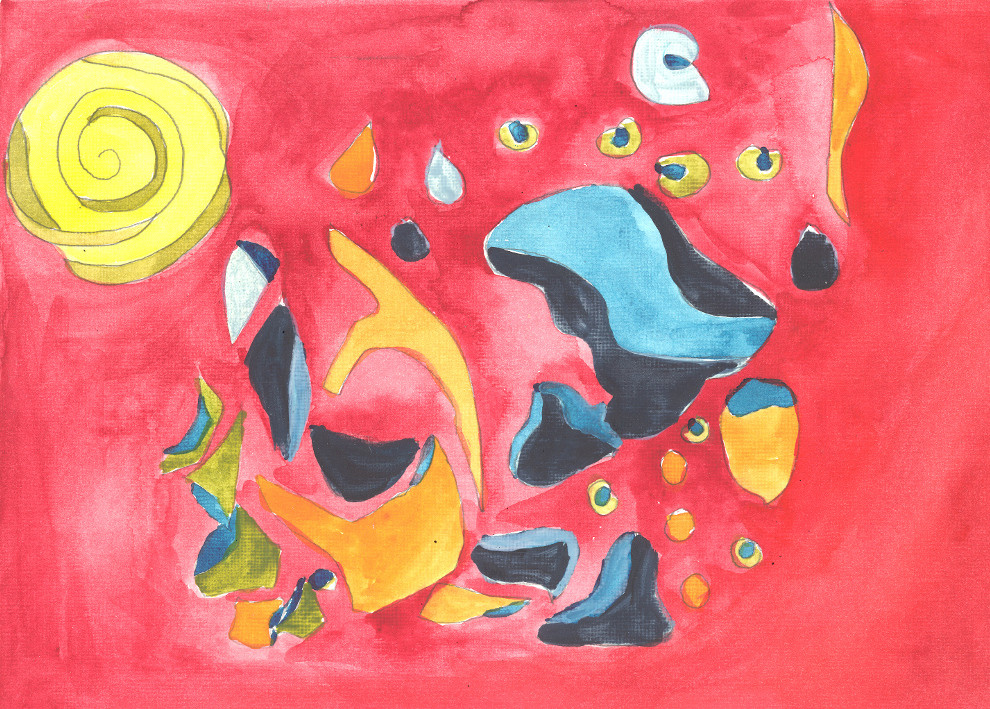
\includegraphics[width=17cm]{Anna_cover_smj}
    } 
\vspace{2cm}

%\begin{figure}[!ht]
%  \centering
%  \includegraphics[width=10cm]{Anna1_sm.png}  
%\end{figure}

\noindent Lecture notes by Amir Erez 

\noindent Ben Gurion University

% \vspace{1in}
\today

\noindent Watercolors by Anna Ayelet Eppel

\end{adjustwidth}

\pagebreak
%\cleardoublepage
%\begin{adjustwidth}{-1in}{-1in}
\tableofcontents
%\end{adjustwidth}

\mainmatter
%%%%%%%%%%%%%%%%%%%%%%%%%%%%%%%%%%%%%%%%%%%%%%%%%%%%%%%%%%%%%%%%
\setcounter{chapter}{-1}
\chapter{Why study quantum physics?}
\lettrine[lines=3,slope=6pt,nindent=6pt]{\initfamily M}{any} engineering students consider the compulsory physics courses in their degree as a form of refined torture. The reasons for this a numerous; not least because university-level physics is difficult and requires a way of thinking not usually taught in school. Still, probably all engineers would agree that mechanics and electromagnetic courses are important. But why study quantum physics ? Here are some thoughts:

\begin{itemize}
\item You are now investing in your future career. Which means you expect to be working in the next 40 years... Every year, quantum physics plays a larger role in engineering applications: semiconductors, nanotechnology, lasers, superconductors, MRI machines, CCD cameras, computers/mobile phones; this is a partial list of technologies which rely on quantum mechanics to work. As an engineer you should have an understanding of \emph{how} they work. If you don't, you'll be left behind.
\item It's true that engineering software often calculates the quantum effects for you. It's unlikely that you'll need to solve quantum mechanical problems in your professional life. But the difference between an ok engineer and a good engineer is that the latter knows what the software does, not just how to use it.
\item One day we may succeed in building quantum computers. When that day comes, it will bring a technological revolution which hard to imagine. eg. Shor's algorithm factors numbers, which will make current RSA cryptography insecure. Quantum cryptography will allow private communication, ensuring that you and your communication partner are not eavesdropped on. When this revolution happens - you'll definitely need to understand the basics of quantum theory.
\item Why did you go to university in the first place ? Was it just to get your engineering degree and get a job? Or are you interested in expanding your horizons ? Quantum theory is one of the most interesting, bizarre, elegant and successful scientific theories ever made. Unlike most scientific theories, it is not the result of one person - it is the result of the combined effort of the best genius minds of the 20\textsuperscript{th} century. This is your chance to learn it. Take this chance - life is busy - you may not get another.  
\end{itemize}

\noindent How is this engineering course different from a quantum physics course for physics students ?
\begin{itemize}
\item We will solve only the simplest cases possible. They require \emph{understanding} but not a high technical skill. This is partly why in this text I refer to wikipedia often.
\item We will omit some important basic quantum theory topics (such as spin, hydrogen atom, angular momentum) so that we can learn some basic solid state physics. You will need this knowledge later on when you learn about semiconductors.
\item We will not compromise on the fundamentals. When the course is done - you will be able to open any "serious" quantum physics textbook and feel at home. You will not receive a simplified version of quantum mechanics (I don't know if it's even possible). You will receive a quick (and sometimes dirty) introduction to the real thing.
\end{itemize}

%%%%%%%%%%%%%%%%%%%%%%%%%%%%%%%%%%%%%%%%%%%%%%%%%%%%%%%%%%%%%%%%%%%%%%%%%%%%%%%%%%%%%%%%%
\begin{adjustwidth}{}{-1.5in}
\part[Introduction to quantum mechanics]{Introduction to quantum mechanics \vspace{0.5cm}
                \begin{center}
                  \begin{minipage}[l]{12cm}
                      %\vspace{1cm}
						\noindent \parbox{12cm}{
  					    \captionsetup{type=figure}
					    \centering 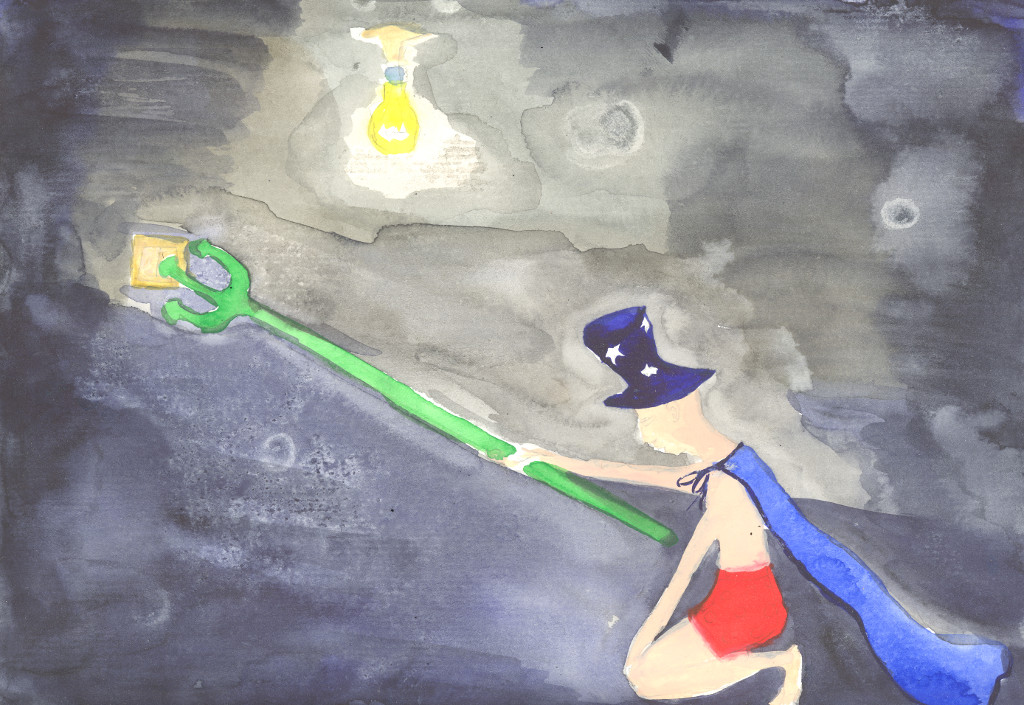
\includegraphics[width=12cm]{Anna1_smj}
					    %\vspace{2cm}
    				} 
                \end{minipage}
                \end{center}
               }
\end{adjustwidth}
\chapter{Experimental background}
\section{The photoelectric effect}
\lettrine[lines=3,slope=6pt,nindent=6pt]{\initfamily A}{t} the end of the 19th century, light was thought to consist of waves of electromagnetic fields which propagate according to Maxwell's equations, while matter was thought to consist of localized particles.

\personfeature[-4in]{Max_Planck_1933}{Max Karl Ernst Ludwig Planck}{1858-1947}{ was a German theoretical physicist who originated quantum theory, which won him the Nobel Prize in Physics in 1918. In 1894 Planck turned his attention to the problem of black-body radiation, commissioned by electric companies to create maximum light from lightbulbs with minimum energy. The question had been explored experimentally, but no theoretical treatment agreed with experiments. Finally, in 1900, he presented his theory, now known as the Planck postulate, that electromagnetic energy could be emitted only in quantized form. Planck stayed in Germany throughout WWI and WWII. When the Nazis seized power in 1933, Planck was 74. In 1945, his son, Erwin, was executed by the Nazis because of his participation in the failed attempt to assassinate Hitler.\href{http://en.wikipedia.org/wiki/Max_Planck}{(Wikipedia)}}
The photoelectric effect was first observed in 1887 by Heinrich Hertz. Hertz found that shining ultraviolet light on metals facilitated the creation of sparks. Later experiments by others, most notably Robert Millikan, observed that shining light on a metal makes it emit electrons, called photoelectrons. But frequencies below a threshold frequency, would not eject photoelectrons from the metal surface no matter how bright the source. The \emph{intensity} of the light only mattered when the \emph{frequency} was higher than the threshold. Below the theshold frequency, no matter how high the intensity, no photoelectrons would be emitted. 

In classical physics, light was considered wave-like. But the energy flux of a wave depends on its amplitude (intensity) according to the Poynting vector $\vec{S} = \frac{1}{\mu_0}\vec{E}\times\vec{B} \propto \vert E \vert^2$. So how was it possible that the high amplitude didn't provide enough energy to eject electrons from the metal ? Einstein was the one to explain the photoelectric effect in one of his famous 1905 papers. He won the Nobel Prize for this work. Einstein's idea was simple: suppose light is composed of \emph{particles} (later called photons), the intensity of the light is proportional to the number of photons. Each photon could knock out one electron, with a relationship between the electron's kinetic energy and the photon \emph{frequency}. Einstein suggested that,
%\begin{equation}
\be
h\nu = \Phi + K \outnote{Einstein's photoelectric equation}
\ee
%\end{equation}
with $\nu$ the frequency of the light, $h$ a constant (later called Planck's constant),$K$ the photoelectron kinetic energy and $\Phi$ a minimal energy (``work function'') below which no photoelectrons are emitted. Since $\Phi>0$, and by definition $K\ge 0$, the photon frequency had to satisfy $\nu \ge \Phi/h$. This link between frequency and energy and the idea that light is composed of \emph{particles} later led to the development of quantum mechanics.

\marginfig[-1.2in]{photoelectric_effect.png}{Photoelectric effect \href{http://en.wikipedia.org/wiki/Photoelectric_effect}{(Wikipedia)} \label{fig:photoelectric_effect}}
\noindent Instead of looking at frequency $\nu$ we can instead think of angular velocity $\omega = 2\pi \nu$ so that
\bea
E &=& h \nu = \hbar \omega \nn
\hbar &=& \frac{h}{2\pi}  \approx 1.05 \times 10^{-34} [J s] \outnote{Planck's Constant}
\eea
Note that the units $[Js]$ are units of \emph{angular momentum} but are also called as units of \emph{action}. $\hbar$ is a quantum of action. As we shall see later in the course, in many ways, the fact that $\hbar \ne 0$ makes the difference between classical physics and quantum physics.

\section{Waves - a brief summary.}

\subsection{The wave equation}
To understand quantum mechanics we must first understand the basics of wave mechanics. A wave propagates energy in time and space. There are two types of waves: transverse and longitudinal. In transverse waves the movement is perpendicular to the direction of the motion of the wave (like in the ocean) whereas in longitudinal waves the movement is parallel (eg. sound waves).\nl
The (simplest) one-dimensional linear wave equation is
\be
\frac{\partial^2 \psi(x,t)}{\partial x^2} = \frac{1}{c^2} \frac{\partial^2 \psi(x,t)}{\partial t^2} \outnote{The wave equation}
\ee
This linear wave equation can be derived from eg:
\begin{itemize}
\item Taking a string, dividing it into differential segments of weights connected by springs and writing Newton's laws. In this case, $c$ is the speed of \emph{sound} in the medium.
\item Playing with Maxwell's electromagnetic equations. In this case $c$ is the speed of \emph{light} in the medium.
\end{itemize}

\subsection{Solution by separation of variables}
We can solve the wave equation by using a technique called ``separation of variables'' which means that we assume that the function $\psi(x,t) = X(x)T(t)$ is a  multiplication of two functions, one that depends solely on time and the other solely on space.
\begin{derivation}{Separation of variables}
\bea
\psi(x,t) &=& X(x)T(t) \nn
\frac{\partial^2 (X(x)T(t))}{\partial x^2} &=& \frac{1}{c^2} \frac{\partial^2 X(x)T(t)}{\partial t^2} \nn
T(t) \frac{\partial^2 (X(x))}{\partial x^2} &=& \frac{1}{c^2} X(x) \frac{\partial^2 T(t)}{\partial t^2} \nn
\frac{1}{X(x)}\frac{\partial^2 (X(x))}{\partial x^2} &=& \frac{1}{c^2} \frac{1}{T(t)} \frac{\partial^2 T(t)}{\partial t^2} = -k^2
\eea
\end{derivation}
Let's look at the last line: on the left we have a expression only of $x$, in the middle we have a expression only of $t$. But $x,t$ are \emph{independent} variables, the only way this equation can work is if both expressions equal a constant, which I call $-k^2$. Now solving each equation separately is easy, by integrating:
\begin{derivation}{Interating the separated variables}
\bea
\frac{1}{X(x)}\frac{\partial^2 (X(x))}{\partial x^2} &=& -k^2 \nn
\frac{\partial^2 (X(x))}{\partial x^2} &=& -k^2 X(x)\nn
X(x) &=& A_+ e^{i k x} + A_- e^{-i k x}\nn
\frac{1}{c^2} \frac{1}{T(t)} \frac{\partial^2 T(t)}{\partial t^2} &=& -k^2 \nn
\frac{\partial^2 T(t)}{\partial t^2} &=& -c^2 k^2 T(t)\nn
T(t) &=& B_+ e^{i ckt} + B_- e^{-i ck t} \nn
\psi(x,t) &=& A_R \cos(k(x - ct) + \phi_R) + \nn
          &+& A_L \cos(k(x + ct) + \phi_L)
\eea
\end{derivation}
Notice that we have two solutions for the wave equation (as expected from a second order equation): one with argument $k(x-ct)$ the other with $k(x+ct)$. The first corresponds to a wave moving right with velocity $c$, the second to a wave moving left. The boundary conditions determine the value of the constants $A_R, A_L,\phi_R, \phi_L$. The argument of the $\cos$ is called the \emph{phase} of the wave.\nl
What about the units ? The argument of the $\cos$ must be dimensionless, so if $x$ is in units of length, then $k$ is in units of length$^{-1}$. So we can make the notation
\be
k = \frac{2\pi}{\lambda} \outnote{Wave-number}
\ee
so that when $x\rightarrow x+\lambda$ then $kx \rightarrow kx + 2\pi$ and the $\cos$ shifts by exactly $2\pi$ which means nothing changes. This is the periodic structure of the wave solution. We call $\lambda$ the wavelength and $k$ the wavenumber.
Let us make the following notation:
\be
\omega = c k \outnote{Linear dispersion}
\ee
Again, since $k$ is in units of length$^{-1}$ and $c$ is in units of length/time then $\omega$ is in units of time$^{-1}$ which is (angular) frequency. Defining
\be
\omega = \frac{2\pi}{T} = 2\pi \nu
\ee
we see that taking $t\rightarrow t+T$ means that $\omega t \rightarrow \omega t + 2\pi$ and again we've shifted the $\cos$ by exactly $2\pi$ which means nothing changes. $T$ is called the period of the wave and $\omega$ its angular frequency. We can also define the frequency $\nu = \frac{\omega}{2\pi} = \frac{1}{T}$.\nl
The relation between the wave frequency $\omega(k)$ and its wavenumber $k$ is called the \emph{dispersion relation} and in the linear wave equation we have linear dispersion.

\subsection{Superposition}
The wave equation is linear (no $\psi^2(x,t)$ or any of its derivatives) and therefore if $\psi_1$ and $\psi_2$ are solutions to the equation, then $\psi = A_1\psi_1 + A_2\psi_2$ is also a solution, with $A_1,A_2$ arbitrary constants. This is the same principle of superposition which appears in Maxwell's equations (which are also linear). Therefore, if there is more than one source generating waves, then the resulting wave is the addition (superposition) of the waves generated by each source.
\begin{figure}[!ht]
  \centering
  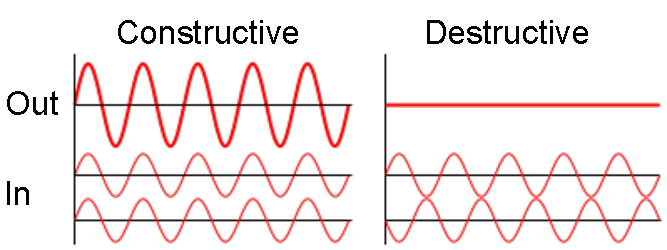
\includegraphics[width=10cm]{Interference_of_two_waves.pdf}  
%  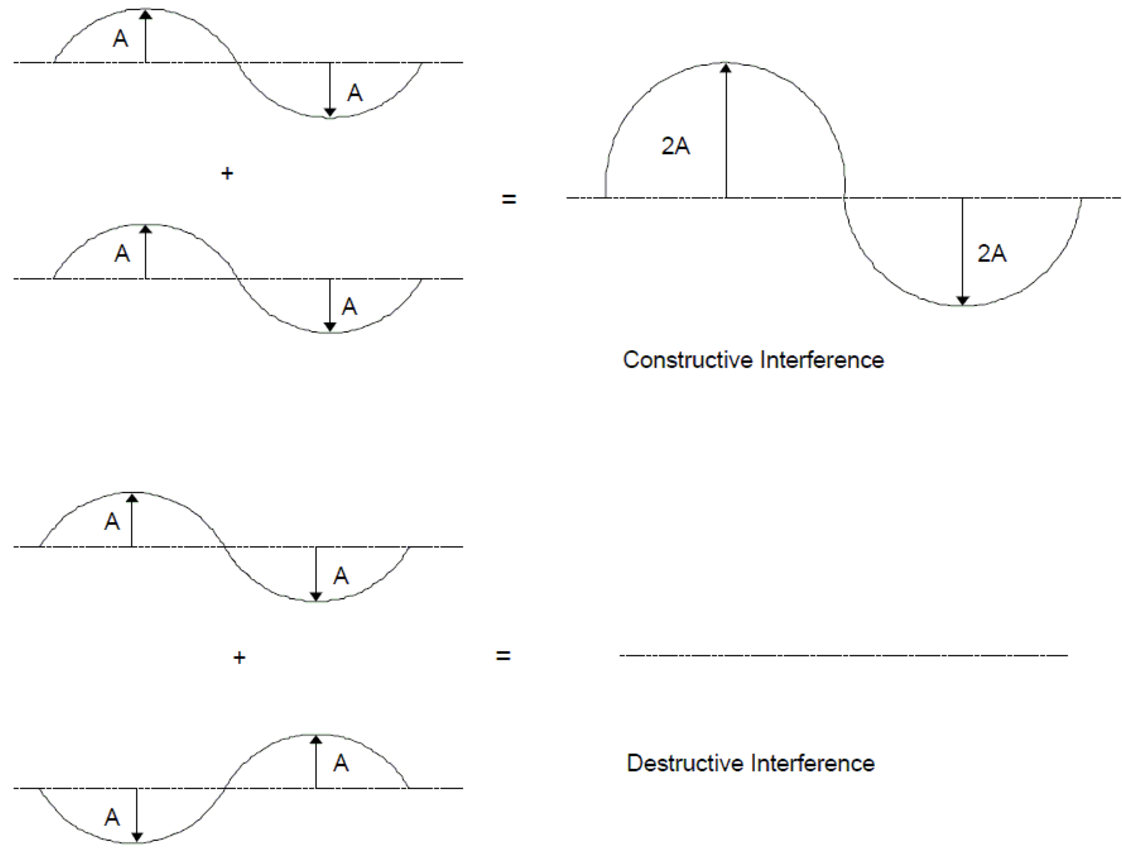
\includegraphics[width=10cm]{superposition.pdf}
  \caption{Interference. \href{http://en.wikipedia.org/wiki/Interference_(wave_propagation)}{(Wikipedia)}}
  \label{fig:superposition}
\end{figure}
Look at Fig. \ref{fig:superposition}, there are places where the two waves add to each other in a positive way - ``constructive interference'', and there are places where the two waves cancel each other ``destructive interference''. We will see later that the same effects play a crucial role in quantum mechanics.

\section{Double-slit experiment: a qualitative description.}
\marginfig[-2.5in]{single_slit_bothj.jpg}{Single slit \label{fig:single_slit}}
Let us first consider when we shine a light wave through a narrow constriction which we call a slit. See Fig. \ref{fig:single_slit}. In both cases, we see a demonstration of the Huygens principle \href{http://en.wikipedia.org/wiki/Huygens\%E2\%80\%93Fresnel_principle}{(Wikipedia)}  (proposed back in 1678 !) which states that every point light reaches becomes a source of a spherical wave. So we can treat the narrow slit (of width $\le$ the wavelength $\lambda$) as a point generating a spherical wave. Now we can graduate to the famous double-slit experiment.
%\marginfig[-1in]{single_slit2.pdf}{aa}
%\begin{figure}
%  \centering
%  \subfigure[]{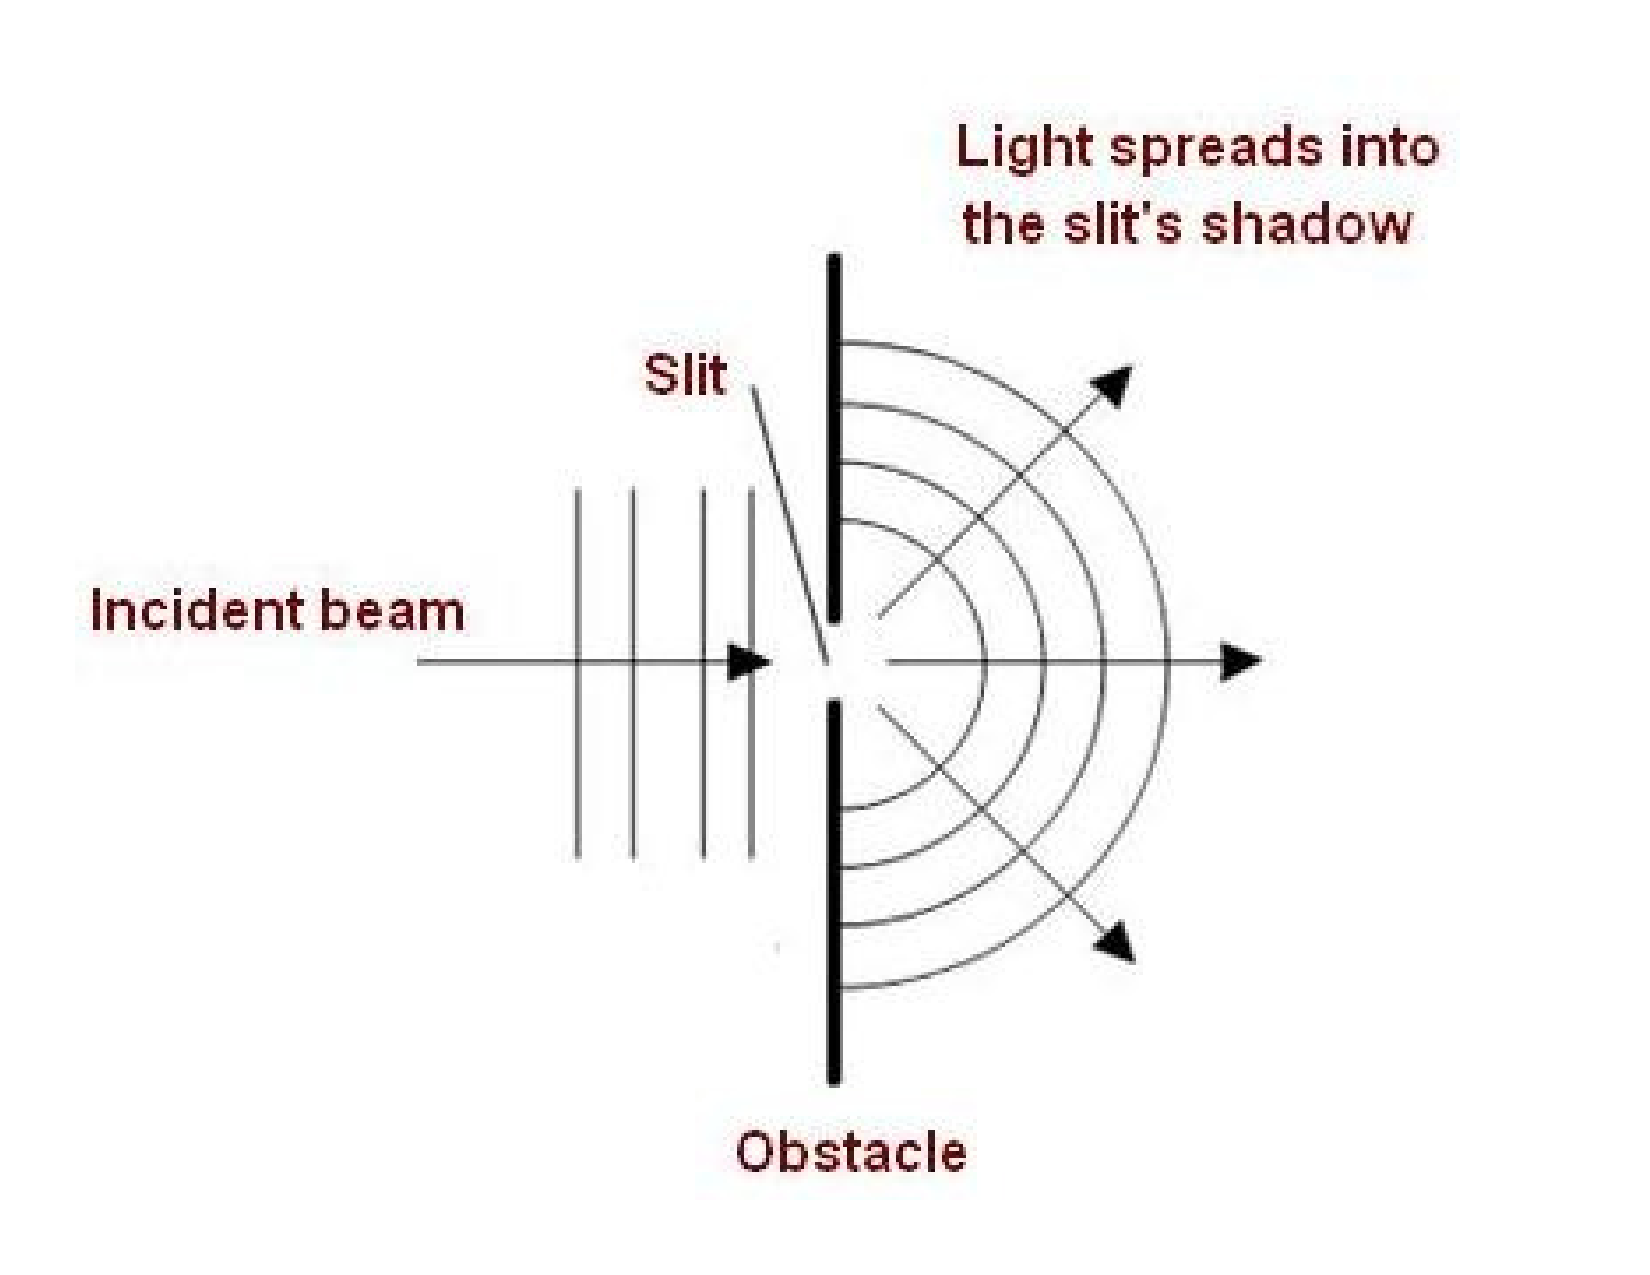
\includegraphics[width=0.49\hsize]{single_slit2.pdf}}
%  \subfigure[]{\includegraphics[width=0.49\hsize]{single_slit.pdf}}
%  \caption{Single slit experiment, \textbf{(a)} schematic ; \textbf{(b)} also works in transverse waves in water.}
%  \label{fig:single_slit}
%\end{figure}
%
The \textbf{double-slit experiment} captures well what is sometimes called the ``wave-particle'' duality of quantum mechanics. A coherent light source such as a laser beam illuminates a thin plate pierced by two parallel slits, and the light passing through the slits is observed on a screen behind the plate. See Fig. \ref{fig:double_slit}.
\marginfig[-1.7in]{doubleslit_both.pdf}{Double slit \label{fig:double_slit}}

%
%\begin{figure}
%  \centering
%  \subfigure[]{\includegraphics[width=0.49\hsize]{doubleslit.pdf}}
%  \subfigure[]{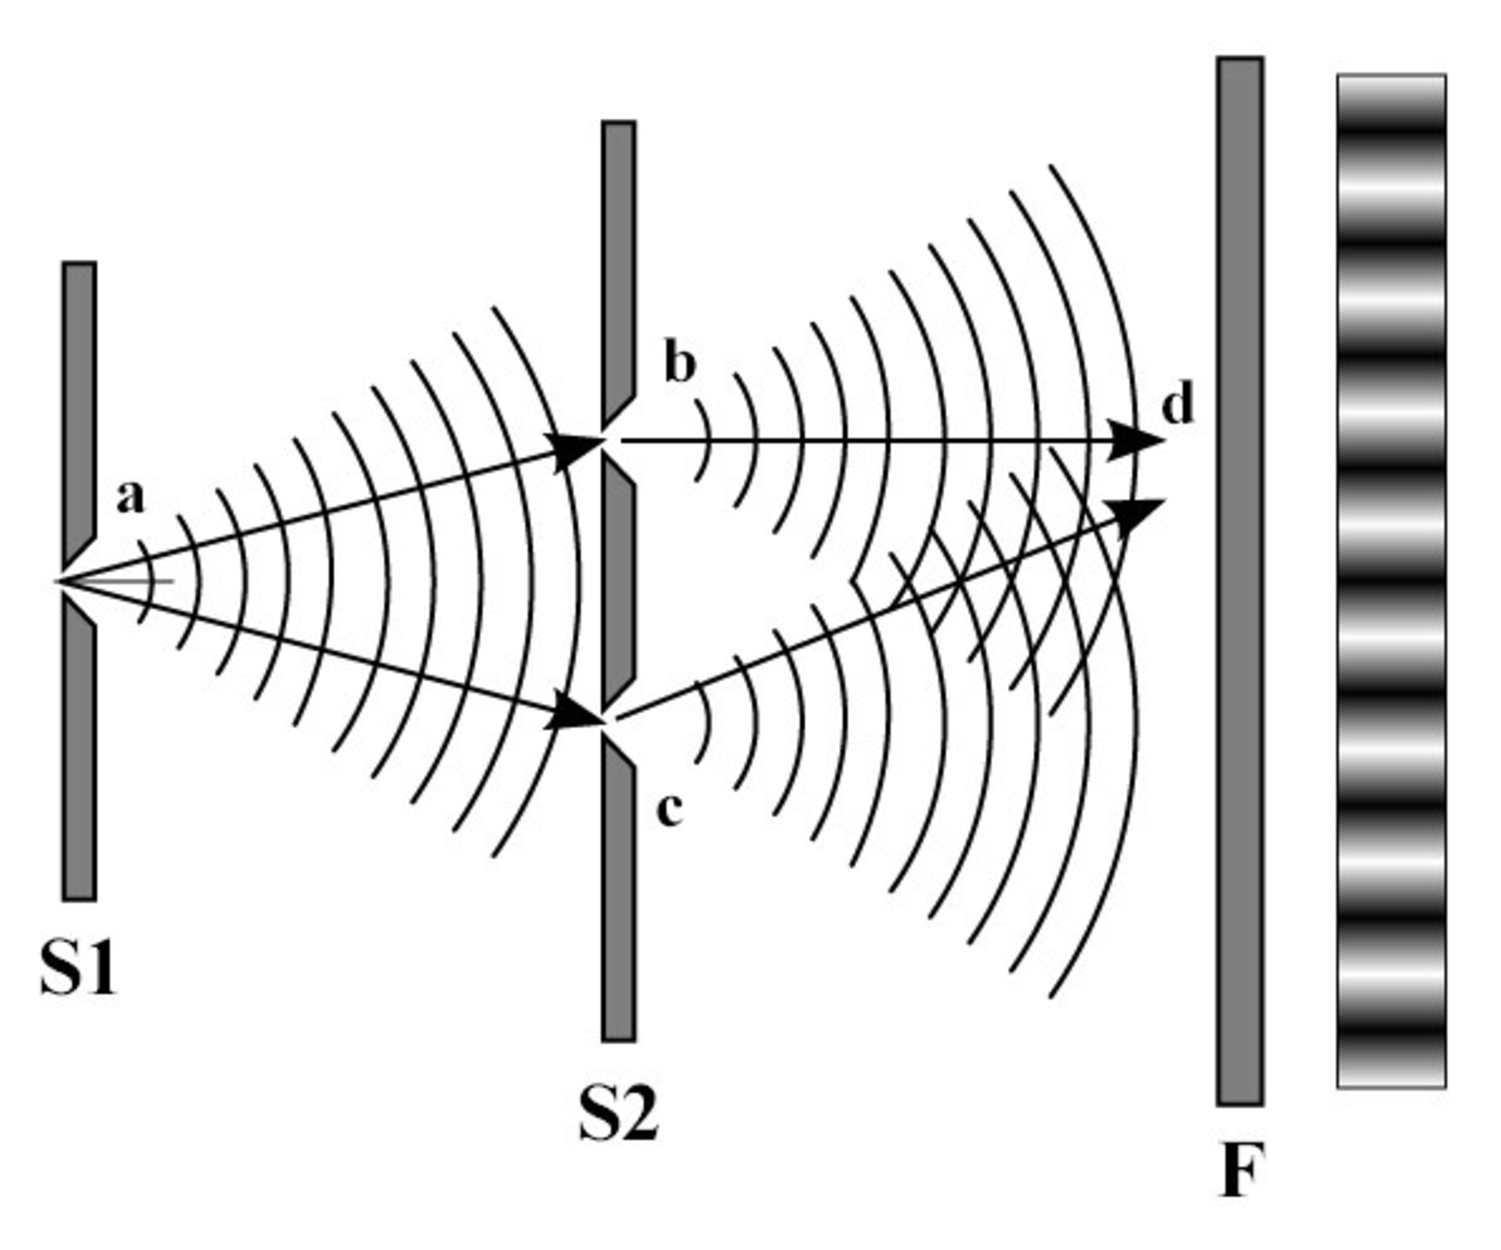
\includegraphics[width=0.49\hsize]{doubleslit2.pdf}}
%  \caption{Double slit experiment.}
%  \label{fig:double_slit}
%\end{figure}
What happens in the experiment ?
The two slits are positioned so that they are the same distance from the light source (left). According to the Huygens principle, both slits act as sources of spherical waves. The wave nature of light causes the spherical waves emitted from the two slits to interfere, producing bright and dark bands on the screen — a result that would not be expected if light consisted strictly of classical particles. If light was a classical particle (eg. tennis ball) then logic says it cannot interfere like a wave. Since we see interference, light must be a wave. But is our analysis correct ?

Let's now start dimming the light source so that it produces less and less light. If light is purely a wave, then all we are doing is decreasing the \emph{intensity} of the light, which means we should see the same interference pattern on the screen, only weaker. Let's take it a step further. Today we have the technology to produce single photons, single particles of light. Say we shine them \emph{one at a time}. Each time, a single photon shoots through the slits (which one?) and is registered on the screen as a dot. The interference pattern disappears ! Light, when we shoot it one photon at a time, behaves as we expect particles to. Surely, a particle \emph{must} pass through either the top slit or the bottom slit ? We repeat the experiment many times, each time noting the location the particle hits the screen. Finally, when we look at the sum of all the experiments, we see the \emph{same interference pattern}. A single particle shows the same interference with itself as waves do. This means that a single particle essentially passes through \emph{both holes}, as a wave will do. Light has both wave-like properties (interference) and particle-like properties (produces a dot and not an interference pattern when single photons are shot). We will see that this observation is not limited to light and will include "matter" as well. This is sometimes called the ``wave-particle duality''.
\noindent In a wave description, the superposition happens at the level of the electric field
\be
\vec{E} = \vec{E}_1 + \vec{E}_2 \outnote{Superposition}
\ee
The electric field vectors come from the same source and are in the same direction (polarization, see below). The light intensity $I$ is proportional to the amplitude squared
\be
I \propto \vert E\vert^2 = \vert E_1 + E_2 \vert^2 = (E_1 + E_2)(E_1^* + E_2^*) = \vert E_1 \vert ^2 + \vert E_2 \vert^2 + E_1E_2^* + E_1^*E_2
\ee
The two free waves have phases $\phi_1(x)$ and $\phi_2(x)$ at point $x$, meaning that the electric fields of the two waves are,
\bea
E_1 &=& A_1 e^{i\phi_1(x)} \nn
E_2 &=& A_2 e^{i\phi_2(x)}
\eea
give intensity
\personfeature[-0.4in]{Huygens}{Christiaan Huygens}{1629-1695}{ was a prominent Dutch mathematician and natural philosopher. He is known particularly as an astronomer, physicist, probabilist and horologist. His work included early telescopic studies of the rings of Saturn and the discovery of its moon Titan, the invention of the pendulum clock and other investigations in timekeeping. He published major studies of mechanics and optics, and a pioneer work on games of chance. Huygens is remembered especially for his wave theory of light, which relies on the principle that the speed of light is finite.
    \href{http://en.wikipedia.org/wiki/Christiaan_Huygens}{(Wikipedia)}}
\bea
I \propto \vert E_1 + E_2 \vert^2 &=& A_1^2 + A_2^2 + 2A_1A_2\cos(\phi_1(x)-\phi_2(x))\nn
[A_1=A_2=\frac{1}{2}A] &\rightarrow & \frac{1}{2}\vert A \vert^2(1+\cos\Delta\phi(x))\nn
 &=& \vert A \vert^2 \cos^2\frac{\Delta \phi(x)}{2}
\eea
this oscillates in the $x$ direction with a stripe pattern like the one produced by the two slit experiment. Note that at $\Delta \phi(x) = 0$ which is $\phi_1(x)=\phi_2(x)$, the intensity is maximal, as we would expect from a superposition of equal phases.

What happens when we shoot the photons one at a time? Each shot has a probability $P(x)dx$ to land on the target screen in location $[x-\frac{dx}{2},x+\frac{dx}{2}]$. After firing many shots, we accumulate a statistic, $\langle I(x) \rangle$, which is very close to the $I(x)$ we have derived from the wave description. As we shoot more and more photons, $\langle I(x) \rangle$ converges to the wave $I(x)$. This is because quantum mechanics is non-deterministic: \emph{a given situation can have several different outcomes, each having a different probability}. By repeating the experiment many times, we gather statistics which converge to a probability distribution.
\section{Linear Polarization}
Take a linearly polarized light beam in the $\vec{e}_p$ direction (pointing in the $x-y$ plane), its electric field is a solution to the wave equation
\be
\vec{E}(z,t) = E_0 \vec{e}_p\, Re[e^{i(kz-\omega t)}]
\ee
with $\vec{e}_p = \cos(\phi)\vec{e}_x + \sin(\phi)\vec{e}_y$; $Re[...]$ takes the real value of the complex exponent, from now on we will omit it in our notation.\nl
The light beam hits a linear polarizer which allows only light polarized in a certain direction, say $\vec{e}_x$, to pass through. So after the polarizer, only the $x$ component of the electric field survives, so that now
\bea
\vec{E}(z,t) &=& E_0 \cos(\phi) \vec{e}_x e^{i(kz-\omega t)} \nn
I &\propto& \vert \vec{E} \vert^2 \propto \vert E_0\vert ^2 \cos^2(\phi) \outnote{Malus' Law}
\eea
The above result is called Malus' law \href{http://en.wikipedia.org/wiki/Malus\%27_law#Malus.27_law_and_other_properties}{(Wikipedia)}.
\marginfig[+0.1in]{wire-grid-polarizer.png}{A wire-grid polarizer converts an unpolarized beam into one with a single linear polarization. \href{http://en.wikipedia.org/wiki/Polarizer}{(Wikipedia)} \label{fig:wire_polarizer}}
What happens at the particle level ? Each photon when it hits the polarizer, has a certain probability to pass through, "transition probability", or to get absorbed/reflected. There is no way to know in advance if a photon will pass through or not, we can only know the probability. When many ($N\gg 1$) photons participate (ie. the "experiment" is repeated many times), the measured intensity - which is the expectation value of the transition, converges to $N\cos^2 \phi$.
\subsection{Spectral Decomposition}
Let us rephrase the polarization experiment in quantum mechanical language. The polarization of a single photon can be written as
\be
\vec{e}_p = \cos(\phi)\vec{e}_x + \sin(\phi)\vec{e}_y
\ee
In cartesian vector form, we can write
\be
\left( \begin{array}{c} \cos \phi \\
              \sin \phi \\
              0
\end{array} \right)  =
\left( \begin{array}{c} \cos \phi \\
              0 \\
              0
\end{array} \right) +
\left( \begin{array}{c} 0 \\
              \sin \phi \\
              0
\end{array} \right)
\ee
Another way to write these vectors is using Dirac's bra-ket notation (which we will discuss later on)
\be
\vert e_p \rangle = \cos \phi \vert e_x \rangle + \sin \phi \vert e_y \rangle
\ee
\personfeature[-0.6in]{Malus}{\'{E}tienne-Louis Malus}{1775-1812}{ was a French officer, engineer, physicist, and mathematician. Malus was born in Paris, France. He participated in Napoleon's expedition into Egypt (1798 to 1801) and was a member of the mathematics section of the Institut d'\'{E}gypte. His mathematical work was almost entirely concerned with the study of light. He studied geometric systems called ray systems, closely connected to Julius Pl\"{u}cker's line geometry. He conducted experiments to verify Christiaan Huygens' theories of light and rewrote the theory in analytical form. His discovery of the polarization of light by reflection was published in 1809 and his theory of double refraction of light in crystals, in 1810. Malus is probably best remembered for Malus' law, giving the resultant intensity, when a polariser is placed in the path of an incident beam. His name is one of the 72 names inscribed on the Eiffel tower.
    \href{http://en.wikipedia.org/wiki/Étienne-Louis_Malus}{(Wikipedia)}}
All three notations are equivalent (though Dirac's is usually easiest to use). The idea is that now, a single photon in the state $\vert e_p \rangle$ is in a superposition of two states, $\vert e_x \rangle$ and $\vert e_y \rangle$, each with its own amplitude. In the quantum mechanical description of the polarization experiment, the probability for the photon to be in a certain state (say $\vert e_x \rangle$) is proportional to the amplitude squared, ie. $\cos^2 \phi$. The polarizer allows only photons in this state to pass through. The idea that the quantum state (of a system, particle, student, universe, whatever) can be written as a superposition of different special (eigen) states of the system is called \textbf{spectral decomposition} \href{http://en.wikipedia.org/wiki/Spectral_decomposition}{(Wikipedia)}, \textbf{which we will use extensively in the course}.
\begin{itemize}
\item A measurement can only give certain, special results which we call \emph{eigen}-values. Here, there are only two possible results: photon has passed through or has not. In contrast, in the classical case, light intensity $I$ is a continuous variable.
\item Each \emph{eigenvalue} corresponds to an \emph{eigenstate}. Here, the two eigenstates are $\vert e_x \rangle$ and $\vert e_y \rangle$. If $\vert e_p \rangle = \vert e_x \rangle$ then we know for sure the photon will pass, if $\vert e_p \rangle = \vert e_y \rangle$ it for sure won't. 
\item If the particle is in one of the eigenstates before the measurement - the result of that measurement is known for sure and it is the eigenvalue.
\item If the state before the measurement is a superposition of eigenvalues, \textbf{only the probability of measuring one of the eigenvalues is known}. That probability is proportional to the square of the coefficient of that eigenstate. This is why, for $\vert e_p \rangle = \cos\phi \vert e_x \rangle + \sin \phi \vert e_y \rangle$ the probability to measure $\vert e_x \rangle$ is $\cos^2\phi$.
\end{itemize}
\section{de Broglie Principle.}
De Broglie, in his 1924 PhD thesis, sought to expand this wave-particle duality from photons (previously thought of as waves) to matter (previously thought of as particles). His idea was that the same way that light (waves) behave like particles, so do matter (particles) behave as waves. If so, then we can define a wavelength for matter. This is the de Broglie wavelength. To define it, we consider that the kinetic energy of a (classical) particle is
\be
E = \frac{1}{2} m v^2 = \frac{p^2}{2m}
\ee
We recall the Einstein-Planck relations for a photon,
\bea
E &=& \hbar \omega \nn
\vec{p} &=& \hbar \vec{k}
\eea
say that, also for matter, the Einstein-Planck photon relations hold
\be
p = \hbar k \quad \longrightarrow \lambda = \frac{2\pi}{\vert \vec{k} \vert} = \frac{h}{\vert \vec{p}\vert}\nn
\ee
so that, even for \emph{matter} eg. electrons, we have
\be
E = \hbar \omega = \frac{p^2}{2m} = \frac{\hbar^2 k^2}{2m} \outnote{de Broglie matter waves}
\label{eq:debro}
\ee
In 1927 at Bell Labs, Clinton Davisson and Lester Germer fired slow-moving electrons at a crystalline nickel target. The angular dependence of the reflected electron intensity was measured and the result could be explained by using de Broglie wavelength for electrons. This was perhaps the first experimental proof that matter indeed behaves as waves.\nl
From thermodynamics we can definite the temperature of a free particle as proportional to its kinetic energy
\be
E_{kin} \propto T
\ee
so that using the de Broglie relation, we have
\bea
k &\propto& \sqrt{\frac{2mE_{kin}}{\hbar^2}} \propto \sqrt{\frac{mT}{\hbar^2}}\nn
\lambda &\propto& \frac{1}{k} \propto \sqrt{\frac{\hbar^2}{mT}} \outnote{Thermal wavelength}
\eea
Note that the \emph{thermal wavelength} $\lambda$ decreases with both temperature and mass. This means that in our "normal" world, where $T$ is large (measured in Kevin $T\approx300K$) and $m$ is large (macroscopic objects), this wavelength becomes very small which means that quantum effects happen on a very small scale. Notice also that this is mathematically similar to taking $\hbar\rightarrow 0$ which is the classical limit. When dealing with low temperatures and small masses (say electrons near $T=0$) then $\lambda$ is large and the quantum effects appear very strongly.
\personfeature[-2in]{Broglie}{Louis-Victor-Pierre-Raymond, 7\textsuperscript{th} duc de Broglie}{1892-1987}{was a French physicist who made groundbreaking contributions to quantum theory. De Broglie had intended a career in humanities, and received his first degree in history. Afterwards, he turned his attention toward mathematics and physics and received a degree in physics. With the outbreak of WWI, he offered his services to the army in the development of radio communications. In his 1924 PhD thesis he postulated the wave nature of electrons and suggested that all matter has wave properties. This concept is known as wave-particle duality or the de Broglie hypothesis. The thesis examiners, unsure of the material, passed his thesis to Einstein for evaluation who endorsed it wholeheartedly. He won the Nobel Prize for Physics in 1929. \href{http://en.wikipedia.org/wiki/Louis_de_Broglie}{(Wikipedia)}}

%%%%%%%%%%%%%%%%%%%%%%%%%%%%%%%%%%%%%%%%%%%%%%%%%%%%%%%%%%%%%%%%%%%%%%%%%%%%%%%%%%%%%%%%%

\chapter{The Schr{\"o}dinger equation}
\personfeature[-4in]{Fourier}{Jean Baptiste Joseph Fourier}{1798-1830}{was a French mathematician and physicist best known for initiating the investigation of Fourier series and their applications to problems of heat transfer and vibrations. He took a prominent part in the French Revolution, serving on the local Revolutionary Committee. He was imprisoned briefly during the Terror but in 1795 was appointed to the \'{E}cole Normale Sup\'{e}rieure, and subsequently succeeded Joseph-Louis Lagrange at the \'{E}cole Polytechnique. Fourier went with Napoleon Bonaparte on his Egyptian expedition in 1798, and was made governor of Lower Egypt and secretary of the Institut d'\'{E}gypte. \href{http://en.wikipedia.org/wiki/Joseph_Fourier}{(Wikipedia)}}
\section{Fourier Transform.}
\lettrine[lines=3,slope=6pt,nindent=6pt]{\initfamily T}{h}e purpose of this section is to quickly discuss Fourier analysis. For more details please refer to specialized maths books.
\subsection{Definition}
We define the 1-d Fourier transform of a function $f(x)$ in the following way:
\bea
f(x) &=& \int_{-\infty}^\infty \frac{dk}{2\pi} e^{i k x} \tilde{f}(k) \nn
\tilde{f}(k) &=& \int_{-\infty}^\infty dx\,e^{ -i k x} f(x) \outnote{Fourier transform}
\eea
The normalization is such that, when applying the transform and its inverse
\bea
f(x) &=& \int_{-\infty}^\infty \frac{dk}{2\pi} e^{i k x} \int_{-\infty}^\infty dx'\,e^{ -i k x'} f(x') \nn
     &=& \int_{-\infty}^\infty dx'\,f(x') \int_{-\infty}^\infty \frac{dk}{2\pi} e^{i k (x-x')}  \nn
     &=& \int_{-\infty}^\infty dx'\,f(x') \delta(x-x') = f(x)
\eea
Where we have exchanged the order of integration and used the following:
\bea
\delta(x-x') &=& \int_{-\infty}^\infty \frac{dk}{2\pi} e^{i k (x-x')}  \nn
f(a) &=& \int_{-\infty}^\infty dx'\, f(x') \delta(x'-a) \outnote{Dirac's delta}
\eea
\subsection{Delta functions}
\personfeature[-0.5in]{Dirac}{Paul Adrien Maurice Dirac}{1902-1984}{was an English theoretical physicist who made fundamental contributions to the early development of both quantum mechanics and quantum electrodynamics. Among other discoveries, he formulated the Dirac equation, which describes the behaviour of fermions and predicted the existence of antimatter. Dirac shared the Nobel Prize in Physics for 1933 with Erwin Schr\"{o}dinger, "for the discovery of new productive forms of atomic theory". Dirac studied electrical engineering at the University of Bristol's engineering faculty and graduated in 1921, but the economic climate of the post-war depression was such that he was unable to find work as an engineer. He completed his Ph.D. in 1926 with the first thesis on quantum mechanics to be submitted anywhere. Dirac is widely regarded as one of the most significant physicists of the 20\textsuperscript{th} century. \href{http://en.wikipedia.org/wiki/Paul_Dirac}{(Wikipedia)}}
Fourier transforming and then exchanging the order of integration is a useful trick which appears commonly in physics.\nl
Let us look at the above. We have defined the \emph{Dirac delta function} as an integral. The delta function $\delta(x-a)$ is identically zero for any $x\ne a$ and is infinite for $x=a$ such that
\be
\int_{-\infty}^{\infty} dx \delta(x-a) = 1
\ee
It can be derived as a limit of zero width Gaussian or Lorentzian. Why is the delta function zero when its argument is nonzero? We will not prove this, but to gain intuition, consider
\be
\int_{-\infty}^{\infty} e^{i k a} dk = \int_{0}^{\infty} \left( e^{i k a} + e^{-i k a}\right) dk = \frac{2}{a} \int_0^\infty \cos(q) dq
\ee
For any $a\ne 0$, the integral (sum) of cosines converges to zero because the different cosines destructively interfere with each other. When $a=0$ then the integral is infinite.
%
\subsection{Application to the wave equation}
Similarly, we can define a transform both in space and time by
\be
\psi(x,t) = \int_{-\infty}^{\infty} \frac{d\omega}{2\pi} \int_{-\infty}^{\infty} \frac{dk}{2\pi} e^{i(kx-\omega t)} \tilde{\psi}(k,\omega)
\ee
Let us look again on the linear wave equation,
\be
\left( \frac{\partial^2}{\partial x^2} - \frac{1}{c^2} \frac{\partial^2 }{\partial t^2} \right) \psi(x,t)=0
\ee
Let us substitute $\psi(x,t)$ with its Fourier transform and exchange the order of derivative and integration
\personfeature[-1in]{Schrodinger}{Erwin Schr\"{o}dinger}{1887-1961}{was an Austrian physicist who developed a number of fundamental results in quantum theory. In subsequent years he repeatedly criticized the conventional Copenhagen interpretation of quantum mechanics. In addition, he was the author of many works in various fields of physics: statistical mechanics and thermodynamics, physics of dielectrics, color theory, electrodynamics, general relativity, and cosmology. In his book "What Is Life?" Schr\"{o}dinger addressed the problems of genetics, looking at the phenomenon of life from the point of view of physics. He paid great attention to the philosophical aspects of science, ancient and oriental philosophical concepts, ethics and religion. He also wrote on philosophy and theoretical biology. According to James D. Watson's memoir, Schr\"{o}dinger's book gave Watson the inspiration to research the gene, which led to the discovery of the DNA double helix structure in 1953. Similarly, Francis Crick also described how he was influenced by Schr\"{o}dinger. \href{http://en.wikipedia.org/wiki/Erwin_Schrödinger}{(Wikipedia)}}
\be
\int_{-\infty}^{\infty} \frac{d\omega}{2\pi} \int_{-\infty}^{\infty} \frac{dk}{2\pi} \left( \frac{\partial^2}{\partial x^2} - \frac{1}{c^2} \frac{\partial^2 }{\partial t^2} \right) \left(  e^{i(kx-\omega t)} \tilde{\psi}(k,\omega)\right)  = 0
\ee
Notice that the function $\tilde{\psi}(k,\omega)$ does not depend on space or time ! So we can act with the derivatives on the exponential,
\bea
\left( \frac{\partial^2}{\partial x^2} - \frac{1}{c^2} \frac{\partial^2 }{\partial t^2} \right)  e^{i(kx-\omega t)} &=& \left((ik)^2 -\frac{1}{c^2}(-i\omega)^2 \right) e^{i(kx-\omega t)} \nn
   &=& \left( -k^2 + \frac{\omega^2}{c^2} \right)e^{i(kx-\omega t)}
\eea
plugging this back into the wave equation we have
\be
\int_{-\infty}^{\infty} \frac{d\omega}{2\pi} \int_{-\infty}^{\infty} \frac{dk}{2\pi} e^{i(kx-\omega t)} \tilde{\psi}(k,\omega) \left( -k^2 + \frac{\omega^2}{c^2} \right)=0
\ee
Since the different Fourier components are orthogonal, each one separately must equal zero. So it remains that for $\tilde{\psi}(k,\omega)\ne 0$,
\be
\left( -k^2 + \frac{\omega^2}{c^2} \right)=0
\ee
again we have derived the dispersion relation for the linear wave equation,
\be
\omega^2 = c^2 k^2
\ee
The Fourier transform is a powerful method to convert differential equations into algebraic ones. It can be used whenever there is translation symmetry in the variable, ie. if the substitution $x\rightarrow x+a$ doesn't affect the physics.

\section{The Schr{\"o}dinger equation}
Let us summarize what we have learned so far.
\begin{itemize}
	\item de Boglie, two-slit: matter and radiation have both particle and wave characteristics.
	\item Quantum processes are probabilistic, as opposed to deterministic.
	\item There is no sense to ask which slit the particle went through. Instead of a trajectory (classical physics: specify $\vec{x}(t),\vec{\dot{x}}(t)$) we use the \emph{quantum state} which is captured in the \emph{wavefunction}.
\end{itemize}
We are looking for an equation that will capture the de-Broglie relations and whos solution will be the quantum state, like Newton's equations capture classical physics and their solution is the trajectory. We also require that this solution will have a probabilistic interpratation.
Let us consider the following:
\be
i\hbar \frac{\partial}{\partial t} \psi(x,t) = \left( -\frac{\hbar^2}{2m}\nabla^2 +V(x,t) \right)\psi(x,t) \outnote{Schr{\"o}dinger's equation}
\label{eq:schred}
\ee
where $\nabla^2 = \frac{\partial^2}{\partial x^2} + \frac{\partial^2}{\partial y^2} + \frac{\partial^2}{\partial z^2}$ and $V(x,t)$ is a time-dependant potential (in this course - $V(x)$ only).\nl
We notice immediately that the equation is
\begin{itemize}
\item Linear, so the superposition principle applies to it.
\item First derivative in time. This is a departure from classical physics and means that if we know the state at time $t$, we can get the state at time $t+dt$.
\end{itemize}
$\psi(x,t)$ which solves the above is called the \emph{wavefunction}.

\subsection{Free particle}
A free particle is a particle that doesn't feel any forces, therefore, it feels a constant potential $V(x)=const$, which we will simplify further to $V=0$. Also, let us look at one spatial dimension only. Now, there is no explicit dependence on time and space in the equation, so we can attempt a Fourier transform to convert it to an algebraic equation.
\be
\left( i\hbar \frac{\partial}{\partial t} + \frac{\hbar^2}{2m}\frac{\partial^2}{\partial x^2} \right) \left( \int_{-\infty}^{\infty} \frac{d\omega}{2\pi} \int_{-\infty}^{\infty} \frac{dk}{2\pi} e^{i(kx-\omega t)} \tilde{\psi}(k,\omega)\right) = 0
\ee
Changing the order of integration and derivative as before,
\be
\int_{-\infty}^{\infty} \frac{d\omega}{2\pi} \int_{-\infty}^{\infty} \frac{dk}{2\pi} e^{-i(kx-\omega t)} \tilde{\psi}(k,\omega) \left( i\hbar (-i\omega) + \frac{\hbar^2}{2m}(-ik)^2\right) =0
\ee
Again, the Fourier components are orthogonal, so each component must satisfy the equation separately.
\bea
\hbar \omega_k &=& \frac{\hbar^2k^2}{2m} \outnote{Free particle dispersion}\nn
E_k &=& \frac{\hbar^2k^2}{2m}
\eea
Notice that this is the de-Broglie relation! The last line defines the energy (or eigen-energy) for the $k$ state as $E_k = \hbar \omega_k$. Notice that since $k$ is not limited and can be any real number, $E_k$ is equally any positive real number, which is the kinetic energy of the free particle. Later we will see how $k$ gets \emph{quantized} meaning that it can only take on certain discrete values, and accordingly the energy will also take discrete values.

\section{Probability and normalization}
We still need a probabilistic meaning to the solution of the Schr{\"o}dinger equation. Going back to our example with the electric field waves, while the wave was $E=E_0 e^{i(kx-\omega t)}$, the intensity which is the measured quantity (number of photons) was $I\propto \vert E \vert^2$. Similarly, let us define the probability to find the particle at location $[x,x+dx]$ at time $t$ is
\be
P(x)dx = \vert \psi(x,t) \vert ^2 dx \outnote{Probability density}
\ee
The probability density must be normalized, so that
\be
\int_{-\infty}^{\infty} P(x)dx = 1 = \int_{-\infty}^{\infty} \vert \psi(x,t) \vert ^2 dx
\ee
so we now have a normalization condition for the wavefunction. This is good, because superposition implies that if $\psi(x,t)$ is a solution, so is $A \psi(x,t)$ with $A$ an arbitary constant. The normalization condition removes the freedom in choosing $A$.
%%%%%%%%%%%%%%%%%%%%%%%%%%%%%%%%%%%%%%%%%%%%%%%%%%%%%%%%%%%%%%%%%%%%%%%%%%%%%%%%%%%%%%%%%
\chapter{Uncertainty principle}
\lettrine[lines=3,slope=6pt,nindent=6pt]{\initfamily L}{e}t us re-examine our solution for the free particle Schr{\"o}dinger equation,
\bea
\label{eq:freewavesol}
\hbar \omega(k) &=& \frac{\hbar^2k^2}{2m} \nn
\psi_{k_0}(x,t)&=& A_{k_0} e^{i(k_0 x-\omega(k_0) t)} \outnote{Free particle wave-function}
\eea
We have derived the dispersion relation directly from the Fourier transform of the equation, whereas the solution $\psi_{k_0}(x,t)$ can be derived from a separation of variables the same way we solved the wave equation. Notice that the solution is itself a "fourier mode", that is, it's a free wave. The Fourier/wave basis is a complete basis which spans the space of functions, meaning that any function (obeying certain conditions we need not discuss here) can be described as a superposition of fourier modes. The Schr{\"o}dinger equation gives us another condition: that the dispersion relation $E(k) = \hbar \omega(k) = \frac{\hbar^2k^2}{2m}$ be obeyed. We discussed a third condition, normalization of the amplitude squared of the wave-function and showed that a free wave cannot be normalized properly.

The free wave solution the way we wrote it, applies to a \emph{single} value of $k=k_0$ and therefore also a single value of $\omega(k_0)$. But we said that $p=\hbar k$ with $p$ the momentum of the wave, so that the wave is defined for a single value of \emph{momentum} $p_0=\hbar k_0$. The probabilistic interpretation means that there is equal probability $P(x) = const$ to be "measured" anywhere: it is "smeared" in space evenly. Notice that we know the momentum of the "particle" perfectly (it is $p_0$), but we do not know its location: it can be anywhere, with equal probability. We can say that instead of it occupying a \emph{position} state, it occupies a \emph{momentum} state. But in reality, we know that particles can exist in certain positions, more or less. How can we define a \emph{localized} particle as opposed to one in a momentum state ?
%
\section{Wave packet description of a free particle.}
\personfeature[-3.2in]{Gauss}{Johann Carl Friedrich Gauss}{1777-1855}{was a German mathematician and physical scientist who contributed significantly to many fields, including number theory, algebra, statistics, analysis, differential geometry, geodesy, geophysics, electrostatics, astronomy, and optics. Gauss was a child prodigy; he had a remarkable influence in many fields of mathematics and science and is ranked as one of history's most influential mathematicians. He made his first ground-breaking mathematical discoveries while still a teenager. He completed Disquisitiones Arithmeticae, his magnum opus, in 1798 at the age of 21, (published 1801). This work was fundamental in consolidating number theory as a discipline and has shaped the field to the present day. Though he did take in a few students, Gauss was known to dislike teaching; several of his students became influential mathematicians, among them Richard Dedekind, Bernhard Riemann, and Friedrich Bessel.  \href{http://en.wikipedia.org/wiki/Gauss}{(Wikipedia)}}
We saw that Eq. \ref{eq:freewavesol} solves the free particle $V=0$ Schr{\"o}dinger equation. Since the equation is linear, the principle of superposition means that any linear combination of such solutions is also a solution. So, quite generally, we may express
\bea
\psi(x,t=0) &=& \sum_k A_k\, e^{ik x} \nn
&=& \int_{-\infty}^\infty \frac{dk}{2\pi} \tilde{\psi}(k)\, e^{ik x} 
\eea
Where in the second line we replaced the discrete set of amplitudes $A_k$ with a continuous function $\tilde{\psi}(k)$. We know the orthogonality relations of the free (fourier) waves so that if we know $\psi(x)$ we can find the fourier amplitudes $\tilde{\psi}(k)$ by integrating both sides
\bea
\int_{-\infty}^\infty dx\, e^{-ik'x} \psi(x,t=0) &=& \int_{-\infty}^\infty dx\, e^{-ik'x}\int_{-\infty}^\infty \frac{dk}{2\pi} e^{ik x} \tilde{\psi}(k)\nn
   &=& \int_{-\infty}^\infty \frac{dk}{2\pi} \tilde{\psi}(k) \int_{-\infty}^\infty dx\, e^{i(k-k') x}\nn
   &=& \int_{-\infty}^\infty dk\, \tilde{\psi}(k) \delta(k-k') \nn
   &=& \tilde{\psi}(k')
\eea
In fact, the single $k_0$ wave solution (eq. \ref{eq:freewavesol}) means that we chose $\tilde{\psi}(k) = 2\pi\delta(k-k_0)$.
So now, instead of choosing a single wave, let us choose the following superposition:
\be
\tilde{\psi}(k) = (2\pi a^2)^{1/4} e^{-\frac{a^2}{4}(k-k_0)^2} \outnote{Gaussian wave-packet}
\ee
Let us check the norm of this "vector":
\bea
\int_{-\infty}^{\infty} \frac{dk}{2\pi}\, \vert \tilde{\psi}(k) \vert^2 &=& \frac{1}{2\pi} \sqrt{2\pi a^2}\int_{-\infty}^{\infty} dk\, e^{-\frac{a^2}{2}(k-k_0)^2}\nn
&=& \frac{1}{2\pi} \sqrt{2\pi a^2} \int_{-\infty}^{\infty} dq\, e^{-\frac{a^2}{2}q^2}\nn
&=& \frac{1}{2\pi} \sqrt{2\pi a^2} \sqrt{\frac{2\pi}{a^2}} = 1
\eea
We see that the wave packet I suggested is normalized. It is a Gaussian wave packet, shown in Fig. \ref{fig:gaussian_kspace}. 
\marginfig[-1.5in]{gaussian_kspace.pdf}{Gaussian in k-space with $a=1,k_0=1$ \label{fig:gaussian_kspace}}

%\begin{figure}[!ht]
%  \centering
%  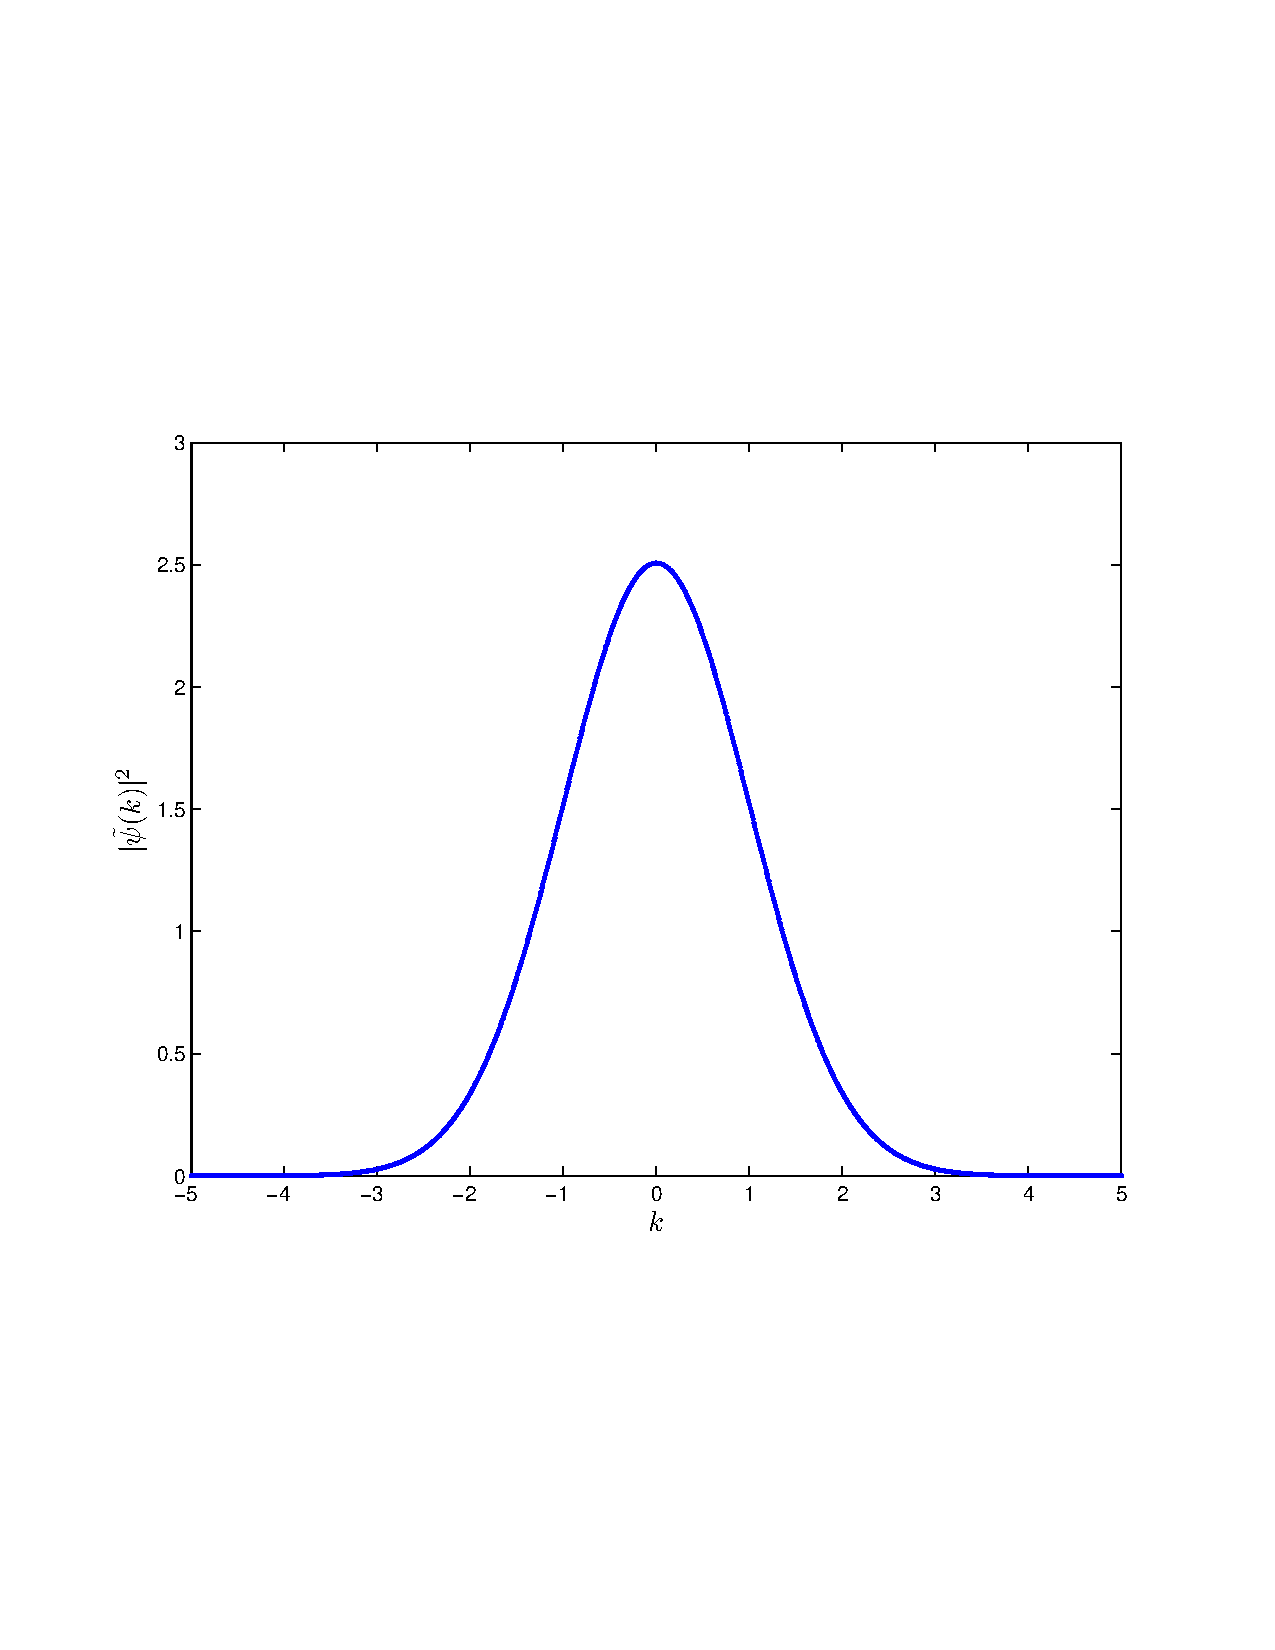
\includegraphics[width=10cm]{gaussian_kspace.pdf}\\
%  \caption{Gaussian in k-space with $a=1,k_0=1$}
%  \label{fig:gaussian_kspace}
%\end{figure}
%\begin{figure}[!ht]
%  \centering
%  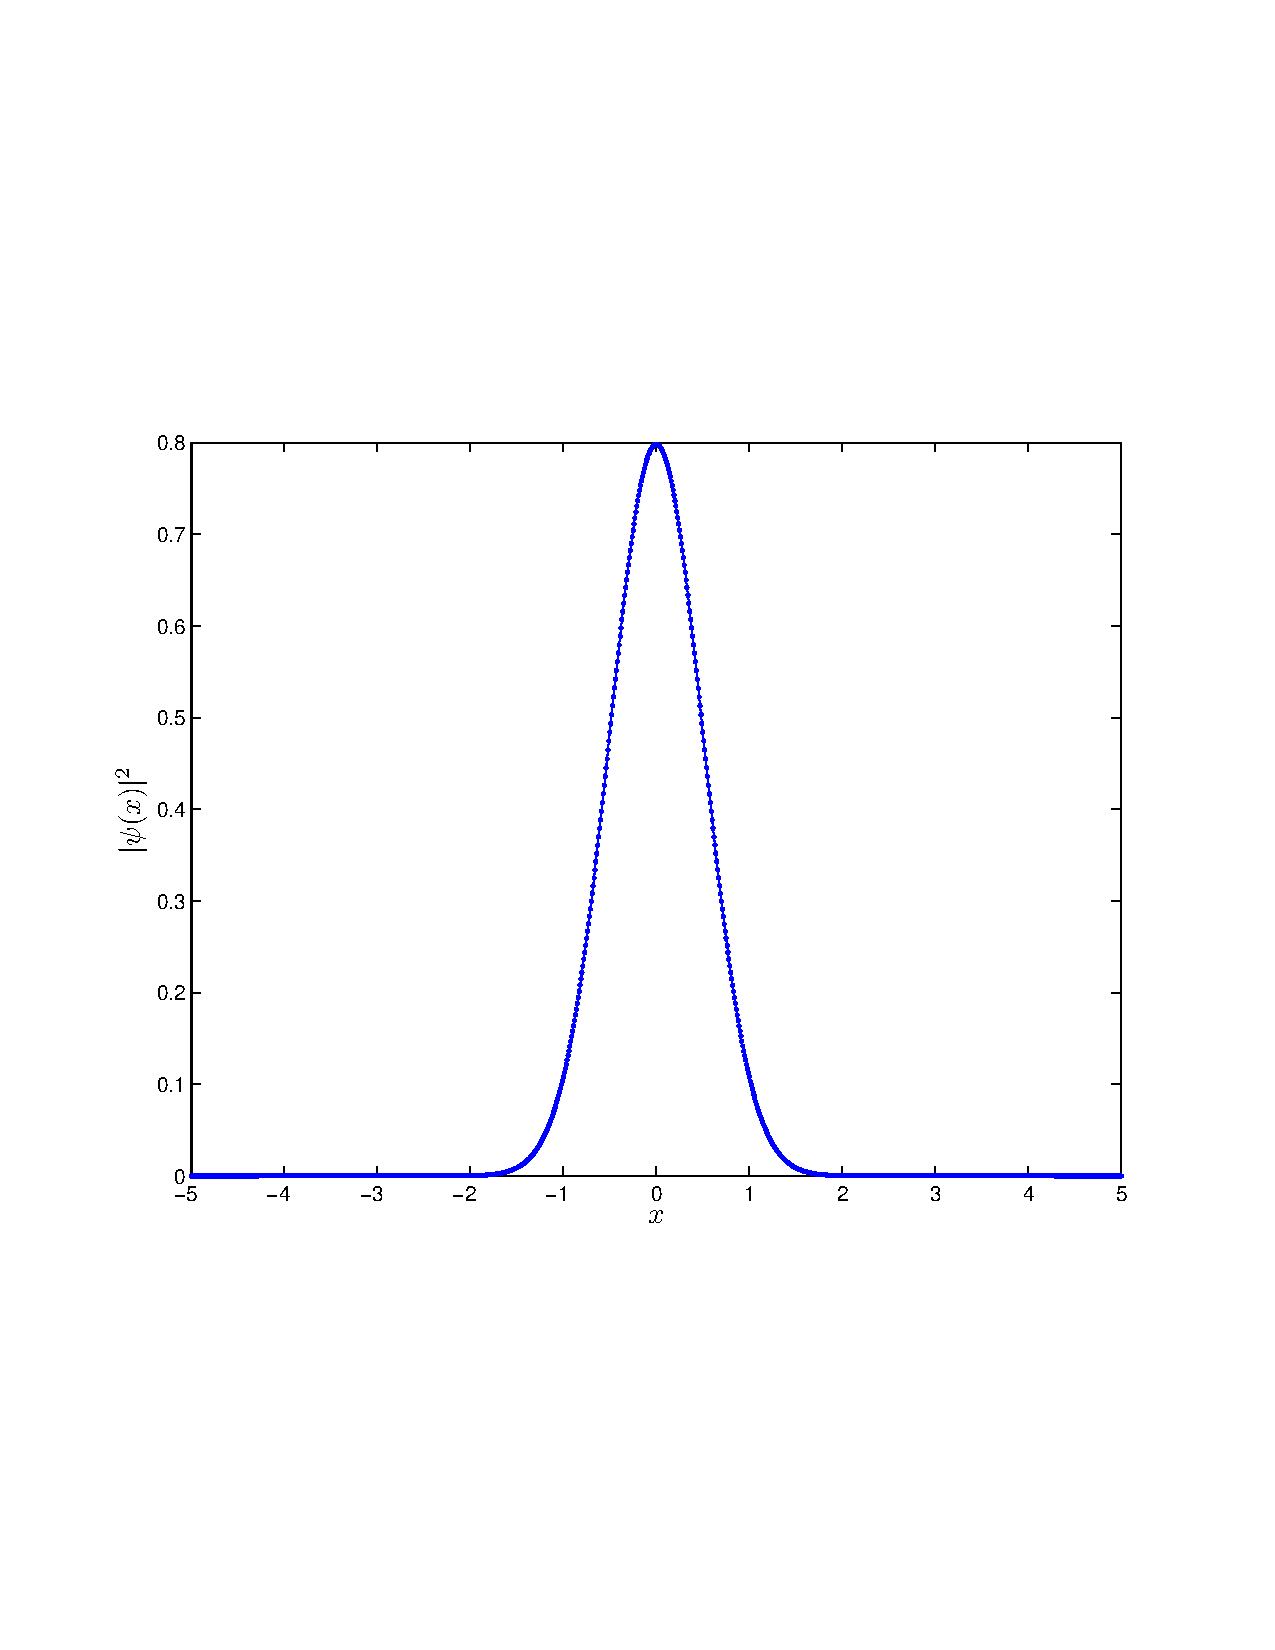
\includegraphics[width=10cm]{gaussian_realspace.pdf}\\
%  \caption{Gaussian in real space with $a=1,k_0=1$}
%  \label{fig:gaussian_realspace}
%\end{figure}

Now let's find $\psi(x)$ by completing the square
\bea
\psi(x) &=& \int_{-\infty}^\infty \frac{dk}{2\pi}e^{ikx}(2\pi a^2)^{1/4} e^{-\frac{a^2}{4}(k-k_0)^2}\nn
   &=& \frac{\sqrt{a}}{(2\pi)^{3/4}} \int_{-\infty}^\infty dk\, e^{-\frac{a^2}{4}(k-k_0)^2+ikx}\nn
-\frac{a^2}{4}(k-k_0-\frac{2ix}{a^2})^2 &=&  -\frac{a^2}{4}(k-k_0)^2 + ix(k-k_0) +\frac{x^2}{a^2} \nn
   &=& -\frac{a^2}{4}(k-k_0)^2 + ikx + (\frac{x^2}{a^2} - i k_0 x) \nn
\psi(x) &=& \frac{\sqrt{a}}{(2\pi)^{3/4}} \int_{-\infty}^\infty dk\,e^{-\frac{a^2}{4}(k-k_0-\frac{2ix}{a^2})^2}e^{-\frac{x^2}{a^2} + ik_0 x}\nn
&=&  \frac{\sqrt{a}}{(2\pi)^{3/4}} \sqrt{\frac{4\pi}{a^2}} e^{-\frac{x^2}{a^2} + ik_0 x}\nn
&=& \left(\frac{2}{\pi a^2}\right)^{1/4}e^{ik_0 x}e^{-\frac{x^2}{a^2}}
\eea
\marginfig[-2in]{gaussian_realspace.pdf}{Gaussian in real space with $a=1,k_0=1$ \label{fig:gaussian_realspace}}
So that, we see that $\psi(x)$ is also normalized (known as the Parseval identity)
\bea
\int_{-\infty}^{\infty}dx\, \vert \psi(x) \vert ^2 &=& \sqrt{\frac{2}{\pi a^2}} \int_{-\infty}^{\infty}dx\, e^{-\frac{2 x^2}{a^2}} \nn
   &=& \sqrt{\frac{2}{\pi a^2}} \sqrt{\frac{\pi a^2}{2}} = 1
\eea
so $\psi(x)$ now constitutes a valid wave-function because its squared amplitude can be normalized. It is also a Gaussian and is plotted in fig. \ref{fig:gaussian_realspace}.
\section{Uncertainty principle for a wave packet.}
In the last section we saw how a particular superposition of different $k$ waves gives rise to a wave-function which is centered around a particular location. Since the square of the wave-function is the probability to find the system ("particle") in that location, we see a very different situation to before: for the free wave, the momentum was sharply defined but the location was anywhere, whereas for the wave-packet, the location is more specific, but the momentum is more vague. Let us quantify this statement.\nl
When we look at a gaussian function, it is useful to think of the width of the Gaussian as the value of $x$ or $k$ that the value of the function gets reduced by $1/\sqrt{e}$ from its peak. So, we have
\bea
\frac{\vert \tilde{\psi}(\Delta k)\vert^2}{\vert \tilde{\psi}(k=0)\vert^2} = \frac{1}{\sqrt{e}} &\longrightarrow & \Delta k = \frac{1}{a} \nn
\frac{\vert \psi(\Delta x)\vert^2}{\vert \psi(x=0)\vert^2}  = \frac{1}{\sqrt{e}} &\longrightarrow & \Delta x = \frac{a}{2}
\eea
We can consider $\Delta x, \Delta k$ the \emph{uncertainty} in $x$ and $k$ because for this range of values, there is a large probability to find the particle. Since $p=\hbar k$ we have $\Delta p = \frac{\hbar}{a}$ and we have the relation, (regardless of the value of $a$),
\be
\Delta x \Delta p = \frac{\hbar}{2} \outnote{Gaussian wave-packet uncertainty relation}
\ee
The above relation is quite robust and is an example of the \emph{Heisenberg's uncertainty principle}. It is important to emphasize that we have derived it, in this example, from a property of the Fourier transform. But the uncertainty principle is something much more general than that. In fact, any kind of wave-packet we could choose, would give a similar uncertainty between $x$ and $k$. Moreover, we note that
\begin{itemize}
  \item Nothing like this exists in classical mechanics, where we know the position and momentum to arbitrary accuracy. In the quantum calculation, there is uncertainty because $\hbar\ne 0$. Again, we see an example where $\hbar$ controls the departure from classical behavior.
  \item We've discussed that the "free wave" with a single $k_0$ corresponds to $\tilde{\psi}(k) = 2\pi\delta(k-k_0)$. But we've also discussed that $\delta(k)$ can be thought of as a Gaussian with width $\rightarrow 0$ keeping its area $=1$. $1/a$ Controls the width of the k-space gaussian so taking $a\rightarrow \infty$ takes the width to zero. Yet the relation $\Delta x \Delta p = \frac{\hbar}{2}$ remains constant, regardless of $a$. So our statement that for the single free wave, the momentum is exact but the position is completely unknown, is in fact a special case of the uncertainty relation we've proven.
  \item We note that the same way that $x,k$ are conjugate Fourier variables, so are $\omega,t$. So we are led to believe there is a relation $\hbar \Delta \omega \Delta t = \Delta E \Delta t = \frac{\hbar}{2}$. Indeed, the same way that the momentum and position cannot be determined to absolute accuracy together, neither is the energy and time. In other words: the experimentalist needs to sit and wait an infinite amount of time to measure the frequency (energy) exactly. There are other such pairs of variables in quantum mechanics, we call them \emph{non-commuting} variables.
  \item One might think that there is something special about our choice of Gaussian wave packets. In fact, any superposition of $k$ states will have similar or worse uncertainty. For an example, see Cohen Tannoudji's book.
\end{itemize}
\personfeature[-7.5in]{Heisenberg}{Werner Karl Heisenberg}{1901-1976}{was a German theoretical physicist and one of the key creators of quantum mechanics. He published his work in 1925 in a breakthrough paper. In the subsequent series of papers with Max Born and Pascual Jordan, during the same year, this matrix formulation of quantum mechanics was substantially elaborated. In 1927 he published his uncertainty principle, upon which he built his philosophy and for which he is best known. Heisenberg was awarded the Nobel Prize in Physics for 1932 "for the creation of quantum mechanics". He also made important contributions to the theories of the hydrodynamics of turbulent flows, the atomic nucleus, ferromagnetism, cosmic rays, and subatomic particles, and he was instrumental in planning the first West German nuclear reactor. Considerable controversy surrounds his work on atomic research during World War II. \href{http://en.wikipedia.org/wiki/Werner_Heisenberg}{(Wikipedia)}}
\section{Time independent Schr{\"o}dinger equation}
Let us limit ourselves to cases when the potential $V(x)$ depends only on space and not on time.\nl
The Schr{\"o}dinger equation is
\be
i\hbar \frac{\partial}{\partial t} \psi(x,t) = \left(-\frac{\hbar^2}{2m} \nabla^2 + V(x)\right)\psi(x,t)
\ee
Since the external potential is constant in time, we expect the total energy to be constant in time since there are no dissipation terms. To solve the equation, let us try again the separation of variables,
\personfeature[-3in]{Hamilton}{William Rowan Hamilton}{1805-1865}{was an Irish physicist, astronomer, and mathematician, who made important contributions to classical mechanics, optics, and algebra. His studies of mechanical and optical systems led him to discover new mathematical concepts and techniques. His greatest contribution is perhaps the reformulation of Newtonian mechanics, now called Hamiltonian mechanics. This work has proven central to the modern study of classical field theories such as electromagnetism, and to the development of quantum mechanics. In mathematics, he is perhaps best known as the inventor of quaternions. He died on 1865, following a severe attack of gout precipitated by excessive drinking and overeating. \href{http://en.wikipedia.org/wiki/William_Rowan_Hamilton}{(Wikipedia)}}
\be
\psi(x,t) = \phi(x) T(t)
\ee
so that
\bea
i\hbar \phi(x)T'(t) &=& \left(-\frac{\hbar^2}{2m}  \phi''(x) + V(x)\phi(x)\right)T(t) \nn
i\hbar \frac{T'(t)}{T(t)} &=& -\frac{\hbar^2}{2m} \frac{\phi''(x)}{\phi(x)} + V(x) = \hbar \omega\nn
\eea
where, again, the two functions must equal a constant which I call $\hbar \omega$ since it has units of energy.\nl
The equation for the time-dependent part reads
\bea
i\hbar \frac{T'(t)}{T(t)} &=& \hbar \omega \nn
T(t) &=& e^{-i\omega t} \times \text{const}
\eea
Similarly, the space-dependent part needs to satisfy
\be
\left(-\frac{\hbar^2}{2m} \nabla^2 + V(x)\right)\phi(x) = \hbar \omega \phi(x) \outnote{Time independent Sch\"odinger equation}
\ee
with the solution, 
\be
\psi(x,t) = \phi(x) e^{-i\omega t}
\ee
The solution above is called a \emph{stationary solution}. This is because the probability $\vert \psi(x,t) \vert ^2$ doesn't change with time. If the system is set in a state $\phi(x)$ it will stay in that state. The state $\phi(x)$ is called a \emph{stationary state} with a well-defined energy $E=\hbar \omega$. Let us define the Hamiltonian operator
\be
\hat{H} = \left(-\frac{\hbar^2}{2m} \nabla^2 + V(x)\right) \outnote{Hamiltonian}
\ee
we use the "hat" to specify explicitly that $\hat{H}$ is an operator. Hamiltonians have many interesting properties and can be studied extensively. Unfortunately, this will be outside the scope of our course. For us, it suffices that the Hamiltonian operator has eigen-values which are the energies of the system. Why? Let's see. Let us recast the spatial part as
\be
\hat{H} \phi(x) = E \phi(x) \outnote{Eigenvalue equation}
\ee
This now looks like an eigenvalue equation, with $\phi(x)$ the eigenstates of $\hat{H}$ with eigenvalue $E$. Only certain energies are allowed, which we label with $E_n$, so that
\be
\hat{H} \phi_n(x) = E_n \phi_n(x)
\ee
We call the $\phi_n(x)$ the energy basis because in this basis the Hamiltonian is diagonal. Working in the energy basis is usually the easier way to solve problems involving time evolution. Why ?\nl
The time evolution of the stationary states is now
\be
\psi_n(x,t) = e^{-iE_n t/\hbar} \phi_n(x) \outnote{Time evolution of stationary states}
\ee
since all our equations are linear, we have, generally,
\be
\psi(x,t) = \sum_n C_n \psi_n(x,t) = \sum_n C_n e^{-iE_n t/\hbar} \phi_n(x)
\ee
Where the coefficients $C_n$ are generally complex. To determine $C_n$ we need to know the system at a given time, say $t=0$, so that
\be
\psi(x,0) = \sum_n C_n \phi_n(x)
\ee
So, quite generally, when given an initial state $\psi(x,t=0)$ we can tell its state at time $t$ by
\begin{itemize}
  \item Decompose $\psi(x,t=0)$ in eigen-functions of the Hamiltonian. This determines $C_n$
  \item Evolve each $\phi_n(x,t) = \phi_n(c,t=0) e^{iE_n t/\hbar}$ according to its eigen-energy.
  \item Recollect the terms to get $\psi(x,t)$.
  \item We note the the energy eignestates form a complete basis, so any (legal) wave-function can be expressed as a superposition of these states. This means that the above algorithm can always be used.
\end{itemize}
This is the power of spectral decomposition: the easy time evolution of eigenstates of $\hat{H}$.
%%%%%%%%%%%%%%%%%%%%%%%%%%%%%%%%%%%%%%%%%%%%%%%%%%%%%%%%%%%%%%%%%%%%%%%%%%%%%%%%%%%%%%%%%

\chapter{Particle in a potential well}
\lettrine[lines=3,slope=6pt,nindent=6pt]{\initfamily W}{e} have seen that the quantum nature of systems gets revealed when the wavelength $\lambda = \frac{2\pi \hbar}{p}$ is comparable to the scale we look at. An example of such a length-scale is when the potential $V(x)$ changes with $x$. When $V(x)$ changes over lengthscales much larger than $\lambda$ then quantum effects are negligible. But if $V(x)$ changes abruptly (ie. potential step) then even very small $\lambda$ should take effect. There is a similar situation in optics: when we look at scales much larger than the wavelength of light, geometric optics usually suffice. But when we looks at lengthscales $\approx \lambda$ we need to use the wave description of light.
%
\section{An infinite potential well in one dimension}
The simplest example we can consider is an infinite potential well in one dimension: a particle in a "box" of length $L$. The confining potential is
\be
V(x) = \left\{ \begin{array}{cc} 
                0 & 0\le x\le L \nn
                \infty & else
\end{array} \right.
\ee
Let us find the energy eigenstates of the system. We need to solve the equation
\be
\hat{H} \phi_k(x) = E_k \phi_k(x)
\ee
with 
\be
\hat{H} = -\frac{\hbar^2}{2m}\frac{\partial^2}{\partial x^2} \outnote{Free particle Hamiltonian}
\ee
this is a free wave, but with the following condition: for the particle to be outside the "box" we need it to have infinite energy, so we require that at the edges of the box, the wave-function vanishes
\be
\phi_k(0) = \phi_k(L) = 0
\ee
Since inside the box the particle is free, the solutions in the box are plane waves,
\be
\phi_k(0 \le x\le L) = A_{k+} e^{ikx}+ A_{k-}e^{-ikx}
\ee
But our boundary conditions imply that
\bea
\phi_k(0) &=& A_{k+} + A_{k-} = 0 \nn
\phi_k(L) &=& A_{k+}e^{ikL} + A_{k-}e^{-ikL} = 0 
\eea
The first condition gives $A_{k+}=-A_{k-}$. So the second condition can be rewritten as
\be
e^{ikL}-e^{-ikL} = 2\sin(kL) = 0
\ee
But $\sin(\theta)=0$ means that $\theta = \pi n$ with $n=\pm 1, \pm2,...$. (The state with $n=0$ is technically allowed but means that the wave-function is identically zero everywhere, which is the trivial solution and teaches us nothing). So we have
\bea
k_n L &=& \pi n \nn
k_n &=& \frac{\pi n}{L} \outnote{Quantization of momenta}
\eea
\subsection{Quantization}
We have reached an important conclusion! That the quantum states satisfying the "zero" boundary conditions on the edges imply that only certain values of $k$ are allowed, which we label by $k_n$. We say the $k$, (or the momentum $p=\hbar k$) is \emph{quantized}. What does it mean ? Remembering that the wavelength $\lambda_n = \frac{2\pi}{k_n}$, we have
\be
\lambda_n = \frac{2\pi L}{\pi n} = \frac{2L}{n}
\ee
\marginfig[-2in]{particle_in_a_box_wavefun.pdf}{First four states of a particle in an infinite well. (From Wikipedia) \label{fig:particle_in_a_box_wavefun}}
we see that (fig. \ref{fig:particle_in_a_box_wavefun}) the allowed waves are ones with wavelength as integer multiples of the size of the well, meaning that we can fit exactly an integer number of waves in the well.
%\begin{figure}[!ht]
%  \centering
%  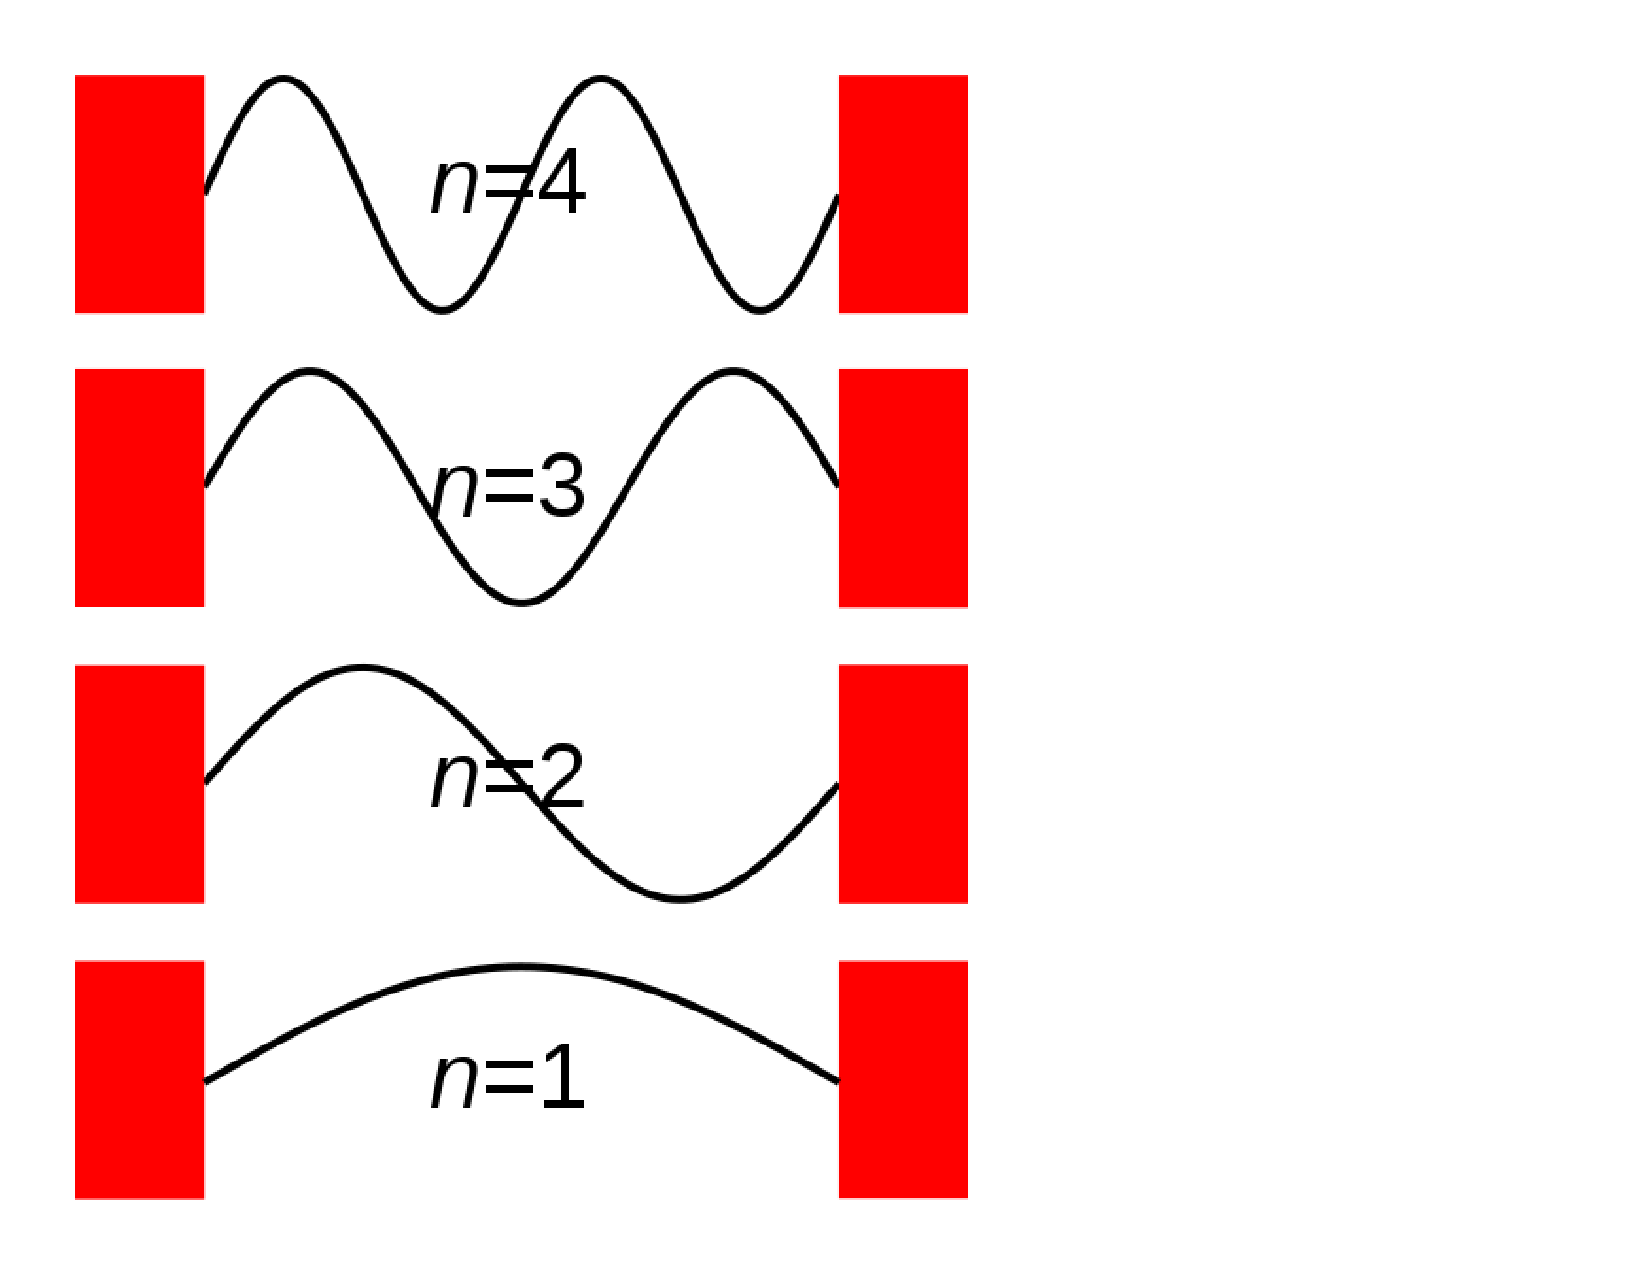
\includegraphics[width=10cm]{particle_in_a_box_wavefun.pdf}\\
%  \caption{First four states of a particle in an infinite well. (From Wikipedia)}
%  \label{fig:particle_in_a_box_wavefun}
%\end{figure}
Moreover, something else has happened. The energies $E_n$ are defined from the dispersion relation according to
\be
E_n = \frac{\hbar^2 k_n^2}{2m} = \frac{\hbar^2 \pi^2 n^2}{2mL^2} \outnote{Quantization of energy}
\ee
so, not only are the momenta quantized, but so are the energies. The quantum particle in an infinite well can only occupy certain discrete energy states as opposed to a continuum of states of a classical particle. To summarize, 
\begin{itemize}
  \item The particle's energy may be only in certain, positive, quanta.
  \item It can never have zero energy, meaning that the particle can never "sit still". This agrees with the uncertainty principle because if we could stop the particle and shrink the well ($L\rightarrow 0$) then we could conceivably measure simultaneously the momentum and position to arbitrary accuracy. But we can't.
  \item Quantization of momentum and energy are contrary to classical mechanics where the particle can have any energy, depending on its momentum.
  \item The particle is more likely to be found at certain positions than at others, whereas a classical particle can be everywhere with equal probability. The particle may never be detected at certain positions, known as spatial nodes.
\end{itemize}
 
\subsection{Normalization}
So far, we've determined that the stationary states of a particle in an infinite potential well are $\phi_n(x) = A_n \sin(k_n x)$. Without extra information, we cannot determine the value of $A_n$. This extra information is the normalization condition, meaning that,
\begin{derivation}{Normalization of infinite well eigenstates}
\bea
\int_{-\infty}^{\infty} dx\, \vert \phi_n(x) \vert ^2 &=& 1 \nn
\int_{0}^{L} dx\,\vert A_n \vert ^2 \sin^2(k_n x) &=& 1 \nn
\int_{0}^{L} dx\,\vert A_n \vert ^2 \frac{1}{2}\left(1-\cos\left(\frac{2 \pi n}{L} x\right) \right) &=& 1 \nn
\vert A_n \vert ^2 &=& \frac{2}{L} \nn
A_n &=& A = \sqrt{\frac{2}{L}}
\eea
\end{derivation}
where in the last line we've chosen $A$ to be real and positive. Making such a choice changes nothing because all physical observations are of $\vert \phi \vert ^2$ or $\vert A \vert ^2$ which is insensitive to the phase of $A$. So, to summarize, we've found the stationary states of an infinite potential well, with
\bea
\phi_n(x) &=& \sqrt{\frac{2}{L}} \sin(k_n x) \outnote{Infinite 1-d well (non-periodic)} \nn
k_n &=& \frac{\pi n}{L} \nn
E_n &=& \frac{\hbar^2 \pi^2 n^2}{2mL^2} 
\eea
To summarize: 
\begin{itemize}
\item Since $\phi_n(x)$ are a set of eigenvalues of $\hat{H}$, they form a complete orthogonal basis, which we now normalized to get a complete orthonormal basis. We call this basis the energy basis.
\item $\phi_n$ are the "unit vectors" in a geometric representation except the space we're dealing with has infinite dimensions.
\item We can use the energy basis to decompose any wave-function $\psi(x)$.
\item The advantage of using the energy basis is that time evolution is easy - each $\phi_n$ evolves with a phase $e^{-i E_n t/\hbar}$ according to its energy eigenvalue $E_n$.
\end{itemize}

\subsection{Time evolution}
Assuming that at $t=0$ the system is prepared at
\be
\psi(x,t=0) = \frac{1}{\sqrt{2}} \sqrt{\frac{2}{L}}\left( \sin(k_1 x) + \sin(k_2 x)\right)
\ee
what is the state of the system at time $t$ ?

\noindent Our life is easy because $\psi(x,t=0)$ has already been written for us as a superposition of stationary states. (Meaning that the coefficients $C_n$ are already known to us, no need to find them). I have also added an extra $\frac{1}{\sqrt{2}}$ term which means $\psi(x,t=0)$ is normalized (because each $\phi_n$ contributes 1 to the norm). So the evolution is trivial, with
\be
\psi(x,t) = \frac{1}{\sqrt{2}} \sqrt{\frac{2}{L}}\left( \sin(k_1 x)e^{-iE_1 t/\hbar} + \sin(k_2 x)e^{-iE_2 t/\hbar}\right)
\ee
Therefore, the probability to find the particle at location $x$, time $t$ is
\bea
P(x,t) &=& \vert \psi(x,t) \vert^2 = \frac{1}{L} \left| \sin(k_1 x)e^{-iE_1 t/\hbar} + \sin(k_2 x)e^{-iE_2 t/\hbar}\right|^2\nn
     &=& \frac{1}{L} \left| \sin(k_1 x) + \sin(k_2 x)e^{-i(E_2-E_1) t/\hbar}\right|^2\nn
     &=& \frac{1}{L} \left( \sin^2(k_1 x) + \sin^2(k_2 x) + 2\cos\left(\frac{E_2-E_1}{\hbar}t\right)\sin(k_1 x)\sin(k_2 x)\right)
\eea
We see immediately that the term $\propto \cos\left(\frac{E_2-E_1}{\hbar}t\right)$ adds an interference term familiar to us from a superposition of waves. \emph{Even though the basis functions evolve trivially with time, their superposition doesn't!} I fact, the system oscillates with a period $T$ which is controlled by the argument of the $\cos$ so that,
\bea
\frac{E_2-E_1}{\hbar}T &=& 2\pi \nn
T &=& \frac{2\pi\hbar}{E_2-E_1}
\eea
Placing the expressions for $E_1$ and $E_2$, we get,
\bea
E_2 - E_1 &=& \frac{\hbar^2}{2mL^2}\left((2\pi)^2 - \pi^2\right) = \frac{3\hbar^2}{2mL^2}\pi^2 \nn
T &=& \frac{4mL^2}{3\pi\hbar} 
\eea
this means that at time $t=T$ the system goes back to exactly the same probability distribution as in time $t=0$. Fig. \ref{fig:infinite_well_time_evolution} plots $P(x,t) = \vert\psi(x,t) \vert ^2$ for times $t=0,\frac{T}{4},\frac{T}{2}$.
\begin{figure}[!ht]
  \centering
  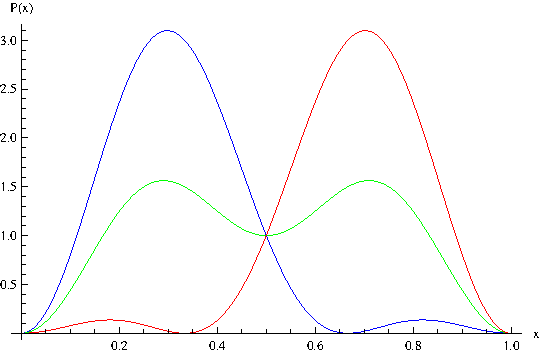
\includegraphics[width=10cm]{infinite_well_time_evolution.pdf}\\
  \caption{Infinite well at times $t=0$ (blue), $t=T/4$ (green), $t=T/2$ (red).}
  \label{fig:infinite_well_time_evolution}
\end{figure}
We can see the following:
\begin{itemize}
\item At time $t=0$ the particle is mostly on the left side of the well.
\item At time $t=T/4$ the particle is spread evenly between the left and right sides.
\item At time $t=T/2$ the particle is mostly in the right side.
\item At time $t=3T/4$ the particle is in the same situation as at $t=T/4$.
\item At time $t=T$ the particle is in the same situation as at $t=0$.
\end{itemize}
We can look at the \emph{expectation value} of the particle location:
\bea
\langle x(t) \rangle &=& \int_{-\infty}^\infty dx\, x\, P(x,t) = \int_0^L dx\, x\, P(x,t) \nn
           &=& L\left( \frac{1}{2}-\frac{16\cos \left(\frac{2\pi t}{T}\right)}{9 \pi ^2}\right)
\eea
We plot $\langle x(t) \rangle$ in Fig. \ref{fig:av_x_infinite_square_well}.
\begin{figure}[!ht]
  \centering
  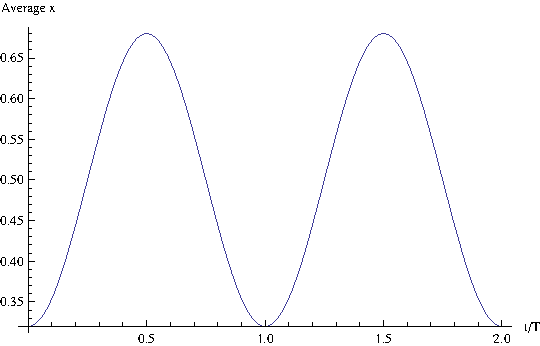
\includegraphics[width=10cm]{av_x_infinite_square_well.pdf}\\
  \caption{Average particle location $\langle x(t) \rangle / L$ vs. $t/T$. We see the periodic oscillations between the left and right hand sides with the particle (on average) exactly at the center ($\langle x(t) \rangle=L/2$) for $t=T/4, 3T/4,...$}
  \label{fig:av_x_infinite_square_well}
\end{figure}

\vspace{0.5cm}
\noindent Notice that if the system were prepared in a single state, say $\psi(x,0) = \sqrt{\frac{2}{L}}\sin(k_1 x)$, then $\langle x \rangle$ would simply $L/2$. Because it was prepared in a superposition of two states - the average location now oscillates around the center with period $T$.
\newpage
\section{Scattering from a potential step}
Our next calculation involves scattering, it teaches us fundamental and non-intuitive quantum behavior. Quantum scattering happens whenever there is an interaction between two things: in our example it is the interaction between a particle (wave) and a potential barrier. In this section, our calculations are different from the infinite well; here we're dealing with a free particle (no constraints) which meets a potential barrier. \textbf{So, in contrast to the infinite well, the "incoming" particle's energy and momentum will not be quantized}. 

\noindent Let us assume the following potential:
\be
V(x) = \left\{ \begin{array}{ccc} 
                0 & -\infty < x\le 0 & \nn
                V_0 &  0 < x < \infty  & V_0>0
\end{array} \right.
\ee
The potential above is called "piecewise" because it's defined in pieces. How do we solve such a situation ? First - we must know what energy the particle is in and where it comes from. This determines the momentum of the particle. Let us assume that the (free) particle has (only kinetic) energy E.
We can define $\psi(x)$ to be piecewise as well, in each "piece" the particle is free:
\be
\psi(x) = \left\{ \begin{array}{cc} 
                A_+  e^{ikx} + A_- e^{-ikx} & -\infty < x\le 0 \nn
                B_+ e^{i\alpha x} + B_- e^{-i\alpha x} &  0 < x < \infty 
\end{array} \right.
\ee
with the momenta determined by the \emph{kinetic} energy,
\bea
E(k) &=& \frac{\hbar^2 k^2}{2m}  \quad \rightarrow  \quad k = \pm \sqrt{\frac{2mE}{\hbar^2}}\nn
E(\alpha)-V_0 &=& \frac{\hbar^2 \alpha^2}{2m}  \quad \rightarrow  \quad \alpha = \pm \sqrt{\frac{2m(E-V_0)}{\hbar^2}}
\eea
To determine the values of the amplitudes $A_+,A_-,B_+,B_-$ we need boundary conditions. Let's try different cases:
\subsection{\texorpdfstring{$E>V_0$}{E>V0}, particle comes from the left}
In this case, both $k$ and $\alpha$ are real numbers. But since the particle comes from the left, we can set $B_-=0$. Now we demand that $\psi(x=0)$ be continuous and so its derivative (the continuity of the derivative is not obvious - in the class ex. you will see an example where it isn't). We have
\bea
A_+ + A_-&=& B_+ \nn
ik(A_+ - A_-) &=& i\alpha B_+
\eea
Solving these equations gives
\bea
\frac{A_-}{A_+} &=& \frac{k-\alpha}{k+\alpha} \equiv r\nn
\frac{B_+}{A_+} &=& 1+\frac{A_-}{A_+} = \frac{2k}{k+\alpha} \equiv t
\eea
The above equations define $r,t$ which are the reflection and transmission (complex) amplitudes. All together, we have,
\be
\psi(x) = A_+ \left\{ \begin{array}{cc} 
                e^{ikx} + r e^{-ikx}& -\infty < x\le 0 \nn
                t e^{i\alpha x} &  0 < x < \infty
\end{array} \right.
\ee
Notice that we've put an overall factor $A_+$ which on principle needs to be determined from the normalization condition but is not well-defined for free waves at a specific energy $E_0$ or wavevector $k_0$. We've discuss this already in the context of the uncertainty principle where a complete certainty in $k$ is complete uncertainty in $x$. We've seen that the wave can be localized in space (and therefore have the normalization integral converge) when dealing with a \emph{wave-packet} so that $k\in[k_0-\Delta k,k_0+\Delta_k]$, or, equivalently, that the energy $E\in[E_0-\Delta E,E_0 + \Delta E]$. In what follows, we assume that the results we derive for a specific $k_0$ apply to a wave-packet with energy \emph{around} $E$. The actual calculation is conceptually simple but technically tedious and gives no extra pedagogic value.\nl
Notice that we've defined a reflection amplitude $r$ and a transmission amplitude $t$. They are the ratio of the wavefunction of the incoming ($A_+$) wave to the part that gets reflected $A_-$ and part that gets transmitted ($B_+$). It is convenient to use these ratios because for them we do not need to be able to normalize the whole wavefunction, which we can't.\nl
Since we've defined the reflected wavefuncion as $r$ times the incoming wave, and the transmitted wavefunction as $t$ times the incoming wave, then the \emph{probability} for the particle to get refrected is $R=\vert r \vert^2$. When we study the probability current later in the course, we will see that the probability for the particle to get transmitted is $T=\frac{\alpha}{k}\vert t \vert ^2$.
Indeed,
\be
R + T = \vert r \vert ^2 + \frac{\alpha}{k}\vert t \vert ^2 = \frac{(k-\alpha)^2}{(k+\alpha)^2} + \frac{4k\alpha}{(k+\alpha)^2} = 1 \outnote{Reflection and transmission coefficients}
\ee
From this we conclude that
\begin{itemize}
\item The total probability of the particle to get transmitted or reflected, $R+T=1$ as should be.
\item Even though the energy is higher than the barrier $E>V_0$, there is still a probability to get reflected. This is quite different from classical mechanics where the $R=0$.
\item When $E\gg V_0$ then $\alpha \approx k$ and then $r\approx 0$ which means when the energy is much higher than the barrier than the classical limit is reached, with zero reflection probability.
\end{itemize}
\subsection{\texorpdfstring{$E<V_0$}{E<V0}, particle comes from the left}
This time, $\alpha$ is imaginary, so that whenever we had $\alpha$ before, we now put $i\alpha$, so that
\bea
\alpha &=& \pm i \sqrt{\frac{2m(V_0-E)}{\hbar^2}}\nn
\frac{A_-}{A_+} &=& \frac{k-i\alpha}{k+i\alpha} \equiv r
\eea
with 
\be
\psi(x) = A_+ \left\{ \begin{array}{cc} 
                e^{ikx} + r e^{-ikx} & -\infty < x\le 0 \nn
                t e^{-\alpha x} &  0 < x < \infty
\end{array} \right.
\ee
We immediately see that inside the barrier, the wavefunction decreases exponentially with a typical length $\sim \frac{1}{\alpha} \sim \frac{1}{\sqrt{V_0-E}}$. This means that the limit $V_0 \gg E$ which is a deep barrier, the length over which the wavefunction decreases is $\sim \frac{1}{\sqrt{V_0}}$. In the limit $V_0 \rightarrow \infty$ the wavefunction dies over a distance $\rightarrow 0$. This justifies the "zero" boundary conditions we used in the infinite well. Fig. \ref{fig:square_barrier} shows both cases, $E>V_0$ and $E<V_0$.
\begin{figure}[!ht]
  \centering
  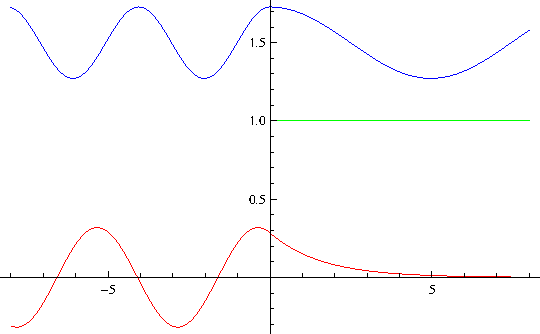
\includegraphics[width=10cm]{square_barrier.pdf}\\
  \caption{Barrier (green) with real part of the wavefunction for case $E>V_0$ (blue, shifted upwards) and $E<V_0$ (red).}
  \label{fig:square_barrier}
\end{figure}
We note that
\begin{itemize}
\item The particle can penetrate the barrier upto a depth $\sim \frac{1}{\alpha}$. This means that if the barrier was short enough, the particle will have a probability to "reappear" behind it.
\item The reflection probability $R=\vert r \vert ^2 = \left\vert\frac{k-i\alpha}{k+i\alpha} \right\vert^2 = 1$ which means the particle \emph{is definitely} getting reflected. This means that the transmission probability $T=1-R=0$ is zero. When we learn about the probability current we will see why having $\psi(x>0)$ a real function means that the probability current is zero. 
\end{itemize}
\subsection{\texorpdfstring{$E>V_0$}{E>V0}, particle comes from the right}
Let us rewrite our solution as
\be
\psi(x) = \left\{ \begin{array}{cc} 
                A_+  e^{ikx} + A_- e^{-ikx} & -\infty < x\le 0 \nn
                B_+ e^{i\alpha x} + B_- e^{-i\alpha x} &  0 < x < \infty
\end{array} \right.
\ee
This time, we set $A_+=$ because the particle is coming from the right. So we have,
\be
\psi(x) = B_- \left\{ \begin{array}{cc} 
                t' e^{-ikx} & -\infty < x\le 0 \nn
                r' e^{i\alpha x} +  e^{-i\alpha x} &  0 < x < \infty
\end{array} \right.
\ee
\bea
r' = \frac{\alpha-k}{\alpha + k}\nn
t' = \frac{2\alpha}{\alpha + k}
\eea
Similar to before. Notice that in terms of energy
\bea
R &=& \left\vert \frac{\alpha - k}{\alpha + k} \right\vert^2 \nn
&=& \left\vert \frac{\alpha/k - 1}{\alpha/k + 1} \right\vert^2 \nn
&=& \left\vert \frac{\sqrt{1-\frac{V_0}{E}}-1}{\sqrt{1-\frac{V_0}{E}}+1} \right\vert^2
\eea
\begin{itemize}
\item Since in this case $V_0<E$ the reflection probability is well defined and is nonzero ! The particle can bounce off the well, very different from classical mechanics.
\item When $E\rightarrow V_0$ then $R\rightarrow 1$ and the barrier is impenetrable !
\item When $E/V_0 \rightarrow \infty$ only then $R\rightarrow 0$ and indeed the particle doesn't get reflected.
\end{itemize}
\section{Tunneling}
Now we have learned what we need to understand tunneling. Assume a potential,
\be
V(x) = \left\{ \begin{array}{cc} 
                0 & -\infty < x\le 0 \nn
                V_0 &  0 < x \le L \nn
                0 &  L < x < \infty
\end{array} \right.
\ee
As before, we can divide the solution $\psi(x)$ to the three sections, with the particle coming from the left with energy $E<V_0$, gives
\be
\psi(x) = A_+ \left\{ \begin{array}{cc} 
                e^{ikx} + r e^{-ikx} & -\infty < x\le 0 \nn
                t_1 e^{-\alpha x}  +... &  0 < x < L \nn
                t_1 t_2 e^{i k x}  &  L < x < \infty
\end{array} \right.
\ee
As before, we can determine the amplitudes $r,t_1,t_2$ by requiring the continuity of $\psi(x)$ and $\psi'(x)$ at the boundaries of the regions. But a qualitative description will suffice. (The "..." is an exponentially small solution which we neglect in a qualitative description but is important when calculating the problem). Fig. \ref{fig:tunneling} shows qualitatively the form of the wavefunction passing through such a barrier. The idea is that if $L\ll \frac{1}{\alpha}$ then there is a probability for the particle to cross the barrier and end up on the other side ! Even though classically it can't. 
\begin{figure}[!ht]
  \centering
  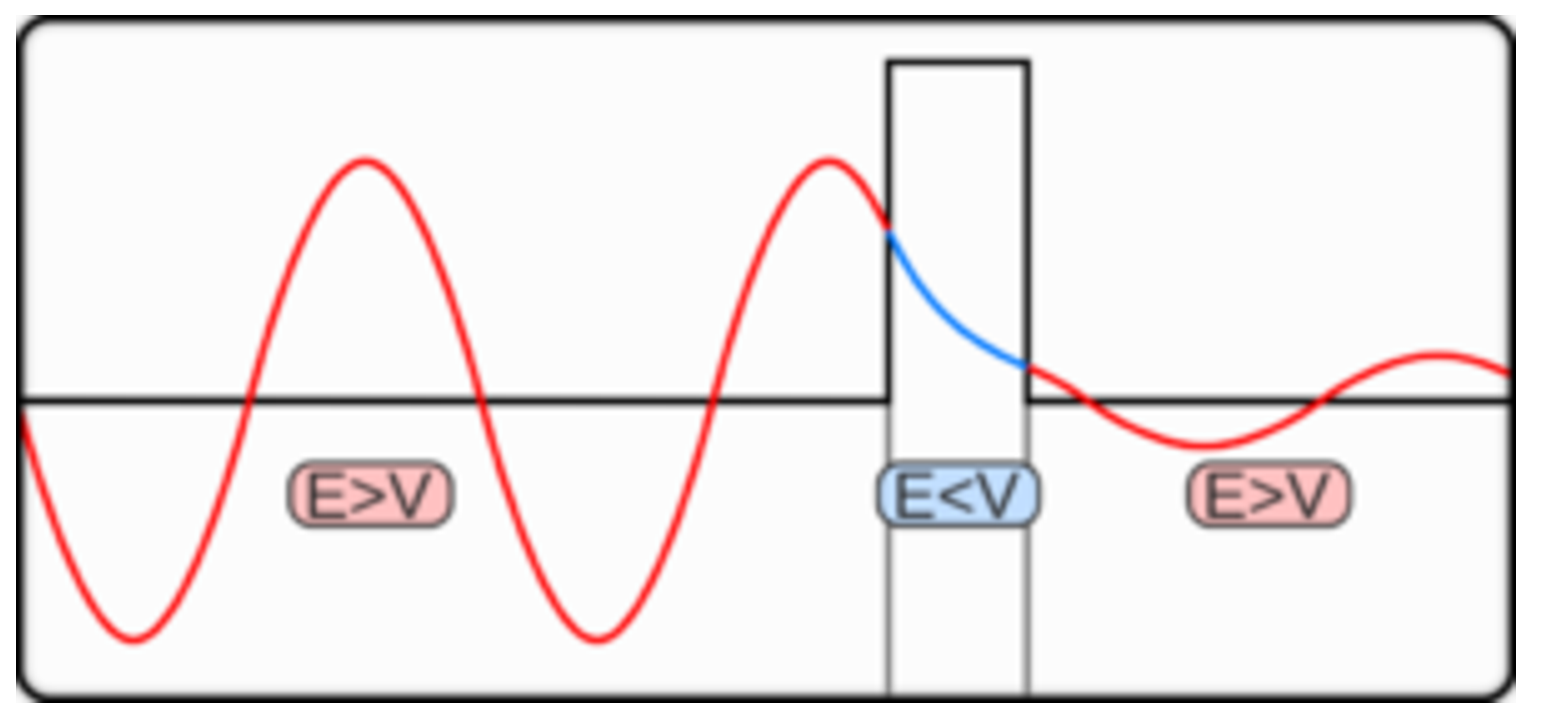
\includegraphics[width=10cm]{tunneling.pdf}\\
  \caption{Schematic depiction of tunneling through a barrier. The particle incident from the left passes a low enough and short enough barrier that it can "leak" to the other side. On the other side of the barrier, it has the same wavelength but an exponentially decreased amplitude. (\href{http://en.wikipedia.org/wiki/Quantum_tunnelling}{Wikipedia})}
  \label{fig:tunneling}
\end{figure}
Let's make a simple calculation to see how such an effect can work in today's nanoscale microchips. Let's assume that we require the tunneling probability to be smaller than the thermal activation probability. This means that
\be
\exp[-2\frac{\sqrt{2m(V_0-E)}}{\hbar}L] < \exp[\frac{V_0-E}{k_B T}]
\ee
Now we assume that the barrier is such that $V_0-E \approx 1$[eV] and room temperature so that $k_B T = 26*10^{-3}$[eV]. Next, we use $\hbar c=197$[eV nm] and $mc^2=511*10^3$[eV]. This means that
\bea
\frac{mc^2}{\hbar c} \sqrt{V_0-E} L &>& \frac{1}{2\sqrt{2}}\frac{V_0-E}{k_B T} \nn
L &>& \frac{1}{2\sqrt{2}}\frac{1000}{26}\frac{197}{\sqrt{511*10^3}}[nm]\approx 3.7[nm]
\eea
So that for barriers of width $L<4$[nm] and of height $V_0-E\approx 1$[eV] there is strong competition between thermal effects and quantum effects !\nl
In VLSI circuits, tunneling is a main cause of a phenomenon known as current leakage. It is also used for flash memory. In microscopy, a Scanning Tunneling Microscope (STM) uses the exponential dependence of the tunneling probability to measure surfaces with incredible accuracy (being able to image single atoms !). Fig. \ref{fig:STM} shows an STM image of a semiconductor with single molecule resolution ! The STM can be used to etch the surface and carve out complex structures.

\begin{figure}[b]
    \inneralign{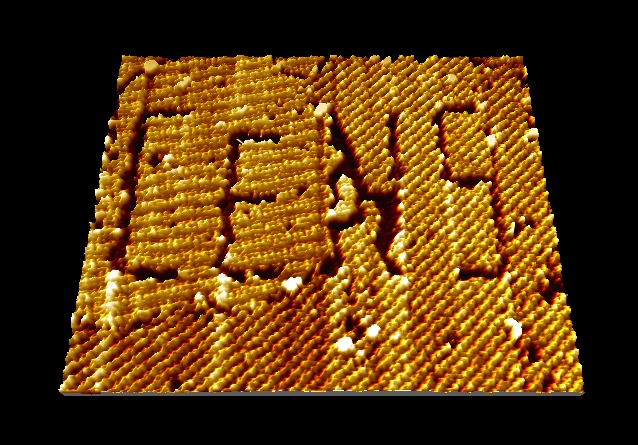
\includegraphics[width=15cm]{Cens_nanomanipulation3d_Trixler.jpg}}
    
    \caption{\label{fig:STM} Nanomanipulation via STM of a self-assembled organic semiconductor monolayer on graphite, in which the logo CeNS has been written. (\href{http://en.wikipedia.org/wiki/Scanning_tunneling_microscope}{Wikipedia})}
\end{figure}


% wide figure
%\begin{figure}[b]
%    \inneralign{\includegraphics[width=15cm]{pollen.pdf}}
%    \caption{\label{fig:pollen} Scanning electron microscope image of pollen grains from a variety of common plants: sunflower (Helianthus annuus), morning glory (Ipomoea purpurea), prairie hollyhock (Sidalcea malviflora), oriental lily (Lilium auratum), evening primrose (Oenothera fruticosa), and castor bean (Ricinus communis). (From Wikipedia)}
%\end{figure}

%\begin{figure}[!ht]
%  \centering
%  \includegraphics[width=15cm]{pollen.pdf}\\
%  \caption{Scanning electron microscope image of pollen grains from a variety of common plants: sunflower (Helianthus annuus), morning glory (Ipomoea purpurea), prairie hollyhock (Sidalcea malviflora), oriental lily (Lilium auratum), evening primrose (Oenothera fruticosa), and castor bean (Ricinus communis). (From Wikipedia)}
%  \label{fig:pollen}
%\end{figure}

%%%%%%%%%%%%%%%%%%%%%%%%%%%%%%%%%%%%%%%%%%%%%%%%%%%%%%%%%%%%%%%%%%%%%%%%%%%%%%%%%%%%%%%%%

\chapter{Energy states, degeneracy, fermion statistics}
\section{Infinite well in higher dimensions}
\lettrine[lines=3,slope=6pt,nindent=6pt]{\initfamily I}{n} the previous chapter, we solved an infinite well in one dimension. For a two dimensional well, we have
\be
V(x,y) = V_x(x)V_y(y) = \left\{ \begin{array}{cc}
                                0 & 0\le x \le L_x \, ,\, 0\le y \le L_y\\
                                \infty & else
                                \end{array}
                        \right.
\ee
The separation of variables works also on the $x,y$ variables (and so also on $z$). Giving 
\bea
\phi_{n_x,n_y}(x,y) &=& \sqrt{\frac{4}{L_x L_y}}\sin(k_{n_x} x) \sin(k_{n_y} y)\nn
k_{n_x} &=& \frac{\pi n_x}{L_x} \nn
k_{n_y} &=& \frac{\pi n_y}{L_y} \nn
\vec{k}_{n_x,n_y} &=& k_{n_x}\vec{e}_x + k_{n_y}\vec{e}_y \nn
E_{n_x,n_y} &=& \frac{\hbar^2 \vec{k}_{n_x,n_y}^2 }{2m}
\eea
Let us note the special case of $L_x=L_y=L$ where,
\be
E_{n_x,n_y} = \frac{\hbar^2 \pi^2}{2mL^2}(n_x^2+n_y^2)
\ee
\section{Definition of degeneracy}
Here we are introduced to the concept of \emph{degeneracy} where there is more than one state possible for the same energy. eg. $n_x=1,n_y=2$ and $n_x=2,n_y=1$ both have the same energy. \nl
Similarly, in 3d we have
\be
E_{n_x,n_y,n_z} = \frac{\hbar^2 \pi^2}{2mL^2}(n_x^2+n_y^2+n_z^2)
\ee
Indeed, the states below all have the same energy
\be
\vec{n} = (n_x,n_y,n_z) = (1,1,2)\,;\,(1,2,1)\,;\,(2,1,1)
\ee
with $\vec{n}^2 = n_x^2+n_y^2+n_z^2 = 6$ so that the energy
\be
E = \frac{\hbar^2 \pi^2 \vec{n}^2}{2mL^2} = \frac{6\hbar^2\pi^2}{2mL^2}
\ee
has degeneracy $3$. \nl
The degeneracy of an energy state can be defined beyond potential wells, and can involve many types of systems. States that are degenerate are orthogonal but have the same energy. Moreover, there are two types of degeneracy: accidental and symmetry based. An accidental degeneracy is when two different states have the same energy because certain parameters of a problem have been cooked that way. But the more interesting degeneracies are those originating from symmetry. What we've explored above is exactly such a case, it's the symmetry between the $x$ and $y$ directions which gives us $L_x = L_y$ and therefore a degeneracy. 
\section{Periodic boundary conditions}
It is sometimes useful to think about loops (1d) or tori (2d) etc. instead of lines, squares. These are periodic boundary conditions. In this case, we demand that $\phi(x=0) = \psi(x=L)$ which gives us
\bea
e^{ikL} &=& 1 \nn
kL &=& 2n\pi \outnote{Quantization of momenta - periodic boundary conditions} \nn
k_n &=& \frac{2\pi n}{L} 
\eea
For periodic boundary conditions, the momentum is still quantized, but this time with a factor of "2" vs. the zero boundary conditions of before.

\section{Describing the quantum state}
So far we've been dealing with free (ie. $\frac{dV(x)}{dx} = 0$) electrons, which have only kinetic energy which is momentum squared $\frac{p^2}{2m}$. All electrons have the same mass $m$, so to describe the quantum state of such a "free" electron, the only thing we have is its momentum vector $\vec{p}= \hbar \vec{k}$. In fact, there is another property of electrons we haven't discussed yet: it's called spin, for our purposes the "spin" can be either "up" or "down". We will not discuss further the implications of spin (which are far and wide and can easily fill a whole course).\nl
In this case, we describe the electron state using momentum and spin, we call them the \emph{quantum numbers}.

\section{Pauli exclusion principle}
\textbf{Pauli exclusion principle}: states that two Fermions (eg. electrons, protons, neutrons and other particles, but not photons) cannot occupy the same quantum state.

In our simple system, the energy of the electrons doesn't depend on their spin, so the "up" electron and the "down" electron both have the same energy, $E_k = \frac{\hbar^2 \vec{k}^2}{2m}$. So each momentum state $\vec{k}$ is double degenerate because of the spin. (This degeneracy is because of the symmetry between the "up" and "down" directions). The Pauli principle tells us that,\nl
\textbf{In a specific momentum state, characterized by the wavevector $\vec{k}$ there can be a \emph{maximum} of 2 electrons, one of spin "up" and one of spin "down".}
%
\section{Number of states}
\personfeature[-2.2in]{Pauli}{Wolfgang Ernst Pauli}{1900-1958}{was an Austrian theoretical physicist and one of the pioneers of quantum physics. In 1945, after being nominated by Albert Einstein, he received the Nobel Prize in Physics for his "decisive contribution through his discovery of a new law of Nature, the exclusion principle or Pauli principle," involving spin theory, underpinning the structure of matter and the whole of chemistry. Pauli proposed in 1924 a new quantum degree of freedom (or quantum number) with two possible values, in order to resolve inconsistencies between observed molecular spectra and the developing theory of quantum mechanics. At the end of 1930, shortly after his postulation of the neutrino and immediately following his divorce in November, Pauli had a severe breakdown. He consulted psychiatrist and psychotherapist Carl Jung who, like Pauli, lived near Zurich, and Pauli became one of the psychologist’s best students. \href{http://en.wikipedia.org/wiki/Wolfgang_Pauli}{(Wikipedia)}}
We have seen that the energy levels of a particle in a $d$ dimensional well of volume $L^d$ and with periodic boundary conditions (we can use "zero" boundary conditions as well but the difference is only a numeric factor) are
\bea
E_{\vec{n}} &=& \frac{\hbar^2 \vec{k}_{\vec{n}}^2}{2m} = \frac{\hbar^2 (2 \pi)^2 n^2}{2mL^2} \nn
n^2 &=& \sum_{i=1}^d n_i^2
\eea
Now say we have a \emph{reservoir} of electrons, which is at energy $E_F$, and we can dump electrons from the reservoir to the well so long as they have energy $E<E_F$. How many electrons in the well ?\nl
The Pauli exclusion principle teaches us that each energy level can "house" a maximum of two electrons, one of spin "up" and the other of spin "down". This is because of the spin degeneracy. An energy level is characterized by a set of values $(n_x,n_y,n_z)$ (in three dimensions, in lower dimensions we have only $n_x,n_y$ or only $n_x$). So the question is: how many different combinations of $(n_x,n_y,n_z)$ are there so that 
\be 
n_x^2+n_y^2+n_z^2 \le R^2 = \frac{2m L^2}{(2\pi \hbar)^2} E_F
\ee
In general, this is a hard problem to solve because $n_x,...$ are integers. But if $E_F$ is large enough that we can "miss" a few states, then we can approximate the calculation to the volume of a sphere. So we can ask: how many combinations of $(n_x,n_y,n_z)$ exist in the sphere of radium $R$. We know that the volume of the sphere is
\be
V_{3d} = \frac{4\pi}{3}R^3 
\ee
Let us recall that in the "infinite well" we allowed only $n\geq 1$, which means for the 3-d case, we allow only $n_x,n_y,n_z\geq 1$. Therefore we need only $1/8$ of the sphere because we allow only \emph{positive} $n_x,n_y,n_z$. If we're dealing with \emph{periodic} boundary conditions - loop, torus, etc. - then we take the whole sphere, without the $1/8$ factor. 

\noindent We also remember that each state is twice degenerate so we need to multiply everything by $x$. So the total number of states of energy $\le E_F$ in $3d$ is 
\be
\mathcal{N}_{3d}(E_F) = 2\times \frac{4\pi}{3}R^3  = 2\times \frac{4\pi}{3} \left( \frac{2m L^2}{(2\pi\hbar)^2} E_F\right)^{3/2} = \frac{8\pi}{3}(2m)^{3/2}\left(\frac{L}{2\pi\hbar}\right)^3 E_F^{3/2} \outnote{Number of states, periodic 3d well}
\ee
Similarly, in $2d$, we have
\bea
V_{2d} &=& \pi R^2 \nn
\mathcal{N}_{2d}(E_F) &=& 2\times \pi \frac{2m L^2}{(2\pi \hbar)^2} E_F = 4 \pi m \left(\frac{L}{2\pi\hbar}\right)^2 E_F \outnote{Number of states, "torus" - periodic 2d well}
\eea
(if we have non-periodic boundary we need to multiply by a factor of $1/4$ of a circle).
\vspace{0.5cm}
\noindent In $1d$ the answer is
\bea
V_{1d} &=& 2R \nn
\mathcal{N}_{1d}(E_F) &=& 4\times \left(\frac{2m L^2}{(2\pi \hbar)^2} E_F\right)^{1/2} = 4\sqrt{2m} \left(\frac{L}{2\pi\hbar}\right) \sqrt{E_F} \outnote{Number of states, "loop" - periodic 1d well}
\eea
To summarize, in $d$ dimensions, we have a total of $\mathcal{N}(E_F)$ quantum states with energy $\le E_F$ according to,
\be
\mathcal{N}(E_F) \propto  E_F^{d/2}
\label{eq:N_of_E}
\ee
and in our case, we have one electron per quantum state so the total number of electrons is the number of states,
\be
N = \mathcal{N}(E_F) = \int_0^{E_F} \frac{d\mathcal{N}}{dE} dE
\ee
Notice also that,
\be
\int_0^{E_F} \mathcal{N}\, dE = \frac{1}{d/2+1} N E_F
\ee
\section{Total Energy}
What is the total energy $E_{tot}$ of the electrons in the well ?\nl
The answer is: it's the sum of the energies of all the electrons with energy $<E_F$. So, assuming periodic boundary conditions,
\bea
E_{tot} &=& 2\sum_{k_x,k_y,k_z:\,\frac{\hbar^2 k^2}{2m}\le E_F}\frac{\hbar^2 k^2}{2m}\nn
&=& 2 \sum_{n_x,n_y,n_z:E(\vec{n})\le E_F} E(\vec{n})
\eea
where the factor of 2 comes from the spin degeneracy. The sum above is difficult to calculate directly, let's see how we can simplify it.\nl
First, let us notice that the total number of electrons is simply $\mathcal{N}(E_F)$ because that's the total number of quantum states with energy $\le E_F$ and each quantum state can hold only one electron. Now we note that instead of summing over $n_x...$ we can (approximately) integrate
\be
N = \sum_{n_x,n_y,n_z} = \int dn_x \int dn_y \int dn_z= \int_0^{E_F} \frac{d\mathcal{N}}{dE} dE
\ee
The expression $\frac{d\mathcal{N}}{dE}$ is called the \emph{density of states} and is the derivative of the number of energy states with respect to the energy. According to Eq. \ref{eq:N_of_E} we have
\be
g(E) \equiv  \frac{d\mathcal{N}}{dE} = \frac{d}{2} \frac{\mathcal{N}}{E} \outnote{Density of states}
\ee
Notice that for $2d$ systems the density of states is constant independent of energy  $E_F$.\nl
Now we can use this knowledge to calculate the energy of the well full of electrons upto $E_F$:
\bea
E_{tot} &=&  2\sum_{n_x,n_y,n_z} E(\vec{n})\nn
   &=&  \int_0^{E_F} g(E) E dE \nn
   &\sim&  \frac{d}{2} \int_0^{E_F} E^{\frac{d}{2}-1} E dE \nn
   &\sim& \frac{d}{2} \times \frac{1}{\frac{d}{2}+1} \times E_F N\nn
   &\sim& \frac{d}{d+2} E_F N
\eea
So we have reached a relation between the energy of an electron system (at zero temperature) $E_{tot}$ and the number of electrons $N$ filled from an outside reservoir at energy $E_F$ so that
\be
E_{tot} = \left\{ \begin{array}{cc}
    \frac{1}{3}N E_F & d=1 \\
    \frac{1}{2}N E_F & d=2 \\
    \frac{3}{5}N E_F & d=3 
\end{array} \right.
\ee
Note that this relation holds only when we use the \emph{free electron dispersion relation} $E(k) \propto k^2$.
\section{Fermi momentum}
\personfeature[-5.4in]{Fermi}{Enrico Fermi}{1901-1954}{was an Italian physicist, known for his work on the first nuclear reactor, and for his contributions to the development of quantum theory, nuclear and particle physics, and statistical mechanics. He is one of the men referred to as "father of the atomic bomb". Fermi was awarded the 1938 Nobel Prize in Physics for his work on induced radioactivity by neutron bombardment and the discovery of transuranic elements. His first major contribution was to statistical mechanics. After Pauli announced his exclusion principle in 1925, Fermi followed with a paper in which he applied the principle to an ideal gas, employing a statistical formulation now known as Fermi-Dirac statistics. Today, particles that obey the exclusion principle are called "fermions". Later Pauli postulated the existence of an uncharged invisible particle emitted along with an electron during beta decay, to satisfy the law of conservation of energy. Fermi took up this idea, developing a model that incorporated the postulated particle, which he named the "neutrino". He is widely regarded as one of the very few physicists to excel both theoretically and experimentally. \href{http://en.wikipedia.org/wiki/Enrico_Fermi}{(Wikipedia)}}
Since we know the dispersion relation, we can define the Fermi wavevector $k_F$ so that
\be 
E_F = \frac{\hbar^2 k_F^2}{2m} = \frac{p_F^2}{2m}
\ee
Now we can write the elecron number and the total energy in terms of the Fermi momentum, in $3d$ we have
\bea
N &=& 2\,\sum_{\vert \vec{k}\vert <k_F} 1\nn
  &=& \left(\frac{L}{2\pi}\right)^3 2\times 4\pi\int_0^{k_F} k^2 dk \nn
  &=& \left(\frac{L}{2\pi}\right)^3 \frac{8\pi}{3} k_F^3 \nn
  &=& \left(\frac{L}{2\pi}\right)^3 \frac{8\pi}{3} \left(\frac{2mE_F}{\hbar^2}\right)^{3/2} \nn
  &=& \frac{8\pi}{3}\left(\frac{L}{2\pi\hbar}\right)^3 (2m)^{3/2} E_F^{3/2}
\eea
Notice that the volume of the Fermi sphere is $\frac{4\pi}{3}k_F^3$ and the volume of a single state is $\left( \frac{2\pi}{L}\right)^3$ which means that the number of electrons is,
\be
N = 2\times \frac{\frac{4\pi}{3}k_F^3 = \mbox{Volume of Fermi Sphere}}{\left( \frac{2\pi}{L}\right)^3 = \mbox{Volume of a state}} \quad . 
\ee 
The total energy is,
\bea
E_{tot} &=& 2\,\sum_{\vert \vec{k}\vert <k_F} \frac{\hbar^2 k^2}{2m} \nn
&=& 2\times \left(\frac{L}{2\pi}\right)^3 \frac{\hbar^2}{2m} \times 4\pi\int_0^{k_F} k^2 dk\, k^2\nn
&=& \left(\frac{L}{2\pi}\right)^3 \frac{\hbar^2}{2m} \,\frac{8\pi}{5} k_F^5 \nn
&=& \left(\frac{L}{2\pi\hbar}\right)^3 \,\frac{8\pi}{5} (2m)^{3/2} E_F^{5/2} \nn
&=& \frac{3}{5}N E_F
\eea 
Since the momentum $p_F=\hbar k_F$ we can define the \emph{Fermi velocity}
\be
v_F = \frac{p_F}{m} = \frac{\hbar k_F}{m}  \outnote{Fermi velocity}
\ee
\section{Fermi Energy, Fermi-Dirac distribution}
So far we've spoken about $E_F$ in rather vague terms. In fact, this quantity, called the Fermi energy, has a physical meaning. The Fermi energy is the energy of the most energetic electron - ie. the energy of the electron with the highest $\frac{p^2}{2m}$. We will deal with it more closely when we talk about electrons in a solid. To conclude this subject, we will now discuss the effect of temperature. So far, we've dealt only with systems at zero temperature, where each electron "sits" nicely in its energy level and nothing can move it away. So we can say that if we set an outside energy cutoff of $E_F$, all energy levels $\le E_F$ are occupied and all energy levels $>E_F$ are empty. This means that the \emph{probability distribution} to find an electron of energy $E$ in the system is
\be
P(E) = \theta(E_F-E)
\ee
with $\theta(E-E_F)$ is the Heaviside function.\nl
Now we introduce temperature. Sadly, a proper discussion of temperature is way outside the scope of this course and is a (fascinating) branch of physics called statistical mechanics. What we can say is that temperature means the outside environment can "kick" an electron out of the the energy level it occupies, to a higher level. This means that now some of the electrons with energy $\le E_F$ are "kicked" up to energy $E>E_F$ and therefore the probability to find an electron with energy $>E_F$ is now no longer zero. The probability distribution to find an electron at energy $E$ is given by the Fermi-Dirac distribution and is 
\be
n_{FD}(E) = \frac{1}{e^{\frac{E-E_F}{k_B T}}+1}  \outnote{Fermi-Dirac distribution}
\ee
with $k_B=1.38\times 10^{-23}\, [J/K]$ the Boltzmann constant and $T$ the temperature in degrees Kelvin. Notice that when $T\rightarrow 0$ we have 
\be 
e^{\frac{E-E_F}{k_B T}}\,\longrightarrow_{T=0}\,  \left\{ 
\begin{array}{cc} 
0 & E<E_F \\
\infty & E>E_F
\end{array} \right.
\ee
So that, at zero temperature we retrieve the Heaviside distribution,
\be
 n_{FD}(E)\,\longrightarrow_{T=0}\,  \left\{ 
\begin{array}{cc} 
1 & E<E_F \\
0 & E>E_F
\end{array} \right.
\ee
Fig. \ref{fig:fermi_dirac} shows the Fermi-Dirac distribution for different temperatures. Notice that it changes significantly from a Heaviside function only approximately when $k_B T\ge E_F/10$.\nl
\begin{figure}[!ht]
  \centering
  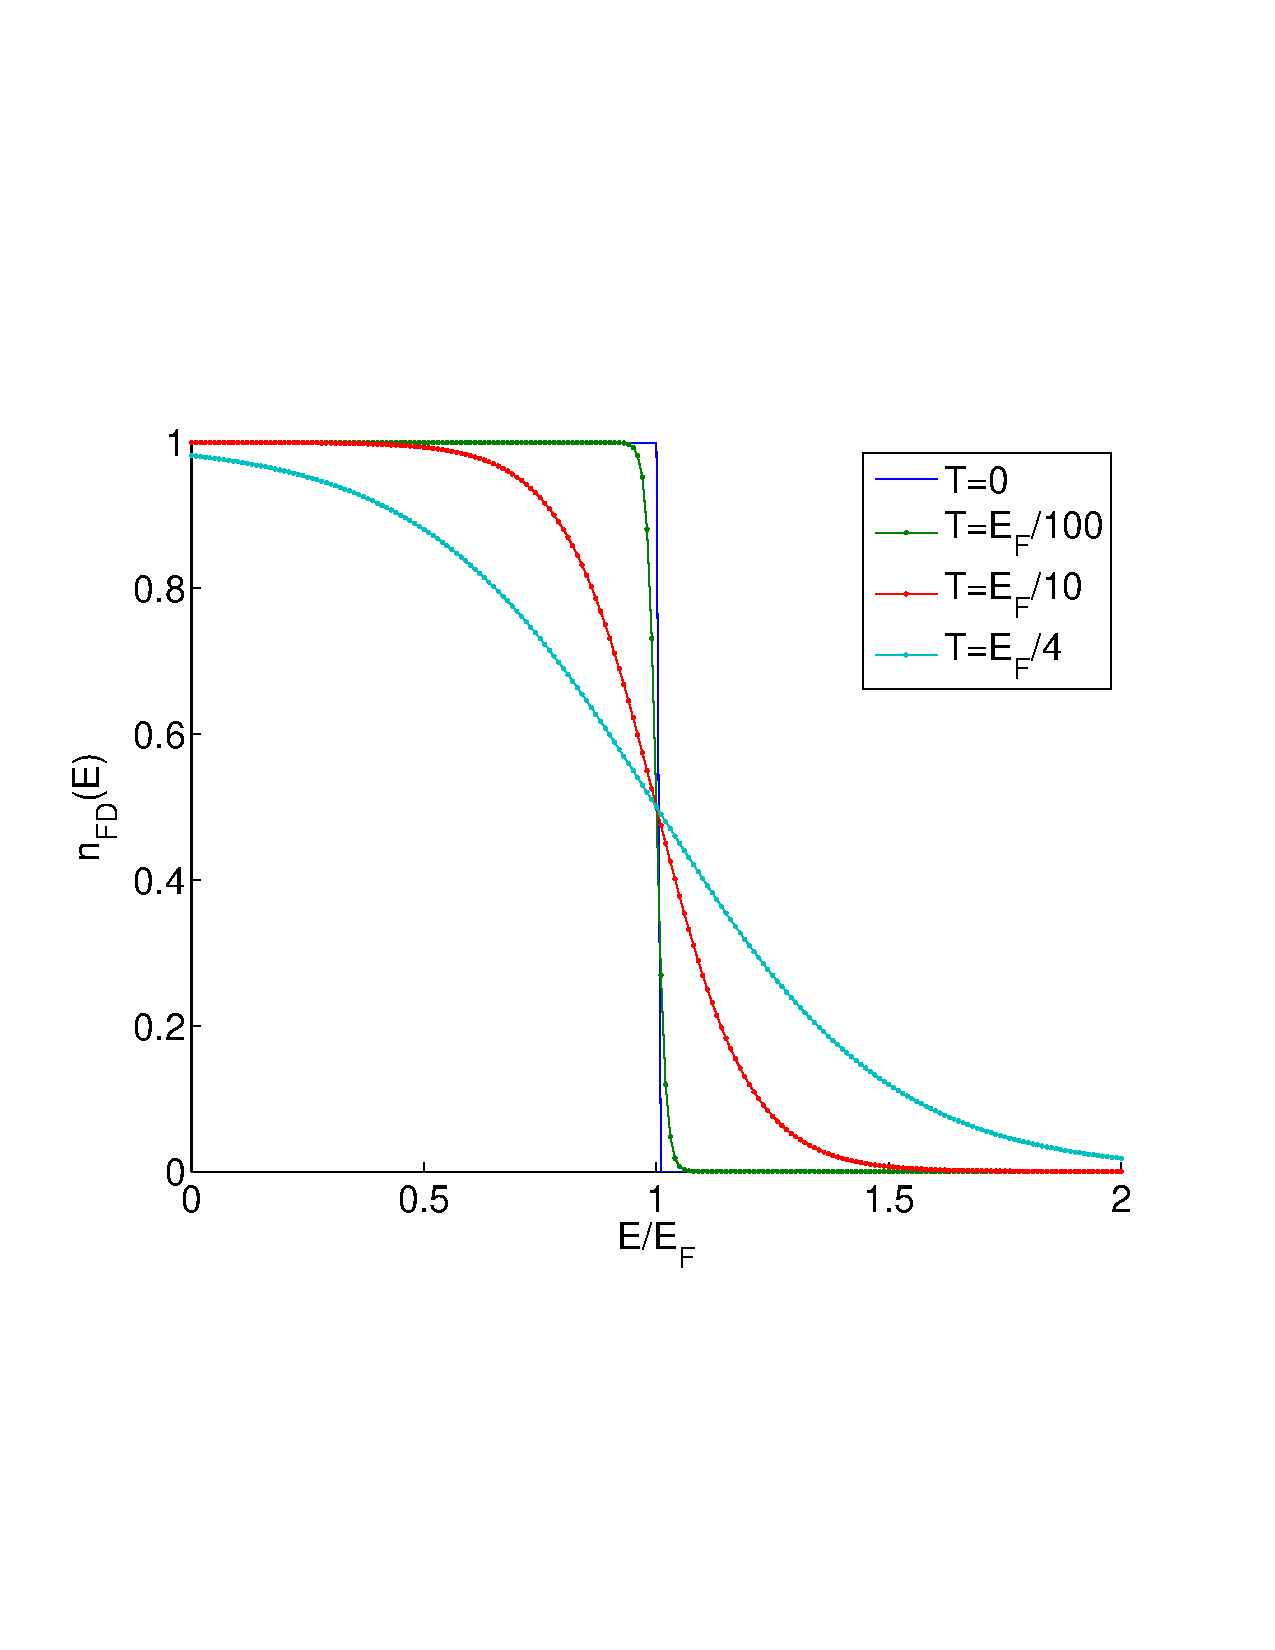
\includegraphics[width=10cm]{fermi_dirac.pdf}\\
  \caption{Fermi-Dirac distribution for temperatures $T=0,E_F/100,E_F/10,E_F/4$.}
  \label{fig:fermi_dirac}
\end{figure}
Let's put some numbers in. The Fermi energy for copper is $\approx 7[eV]$. Room temperature is $300[K] \approx 0.026[eV]$. We see that according to these numbers, and the properties of the Fermi-Dirac distribution, copper at room temperature is almost the same as copper at absolute zero. We will get back to this when we study conduction in the last part of the course.

\section{Probability current}
For completeness, we will now derive a formula of how the probability to find a particle in a certain point at a certain time flows - like a current. Our starting point is the normalized wave-function, which gives a probability density $P(\vec{r},t)$ to find the particle in $\vec{r}$ at time $t$,
\be
P(\vec{r},t) = \vert \psi(\vec{r},t) \vert ^2
\ee
Requiring that no particles can be created or destroyed, means that the current is conserved, therefore obeys the continuity equation,
\be
\frac{\partial}{\partial t} P(\vec{r},t) + \vec{\nabla}\cdot \vec{J}(\vec{r},t) = 0
\ee
with $\vec{\nabla}$ the \emph{divergence} operator and $\vec{J}$ the \emph{probability current}. We proceed to find the probability current directly from the Schr\"odinger equation,
\be 
i\hbar \frac{\partial}{\partial t} \psi(\vec{r},t) = -\frac{\hbar^2}{2m} \nabla^2 \psi(\vec{r},t) + V(\vec{r},t)\psi(\vec{r},t)
\label{eq:Sch1}
\ee
The potential $V(\vec{r},t)$ must be real for the Hamiltonian to be Hermitian. The complex conjugate of the Sch\"odinger equation is
\be 
-i\hbar \frac{\partial}{\partial t} \psi^*(\vec{r},t) = -\frac{\hbar^2}{2m} \nabla^2 \psi^*(\vec{r},t) + V(\vec{r},t)\psi^*(\vec{r},t)
\label{eq:Sch2}
\ee
Multiply both sides of \ref{eq:Sch1} by $\psi^*(\vec{r},t)$ and both sides of \ref{eq:Sch2} by $-\psi(\vec{r},t)$ and add the two equations to get,
\be 
i\hbar  \frac{\partial}{\partial t} \vert \psi(\vec{r},t) \vert^2 = -\frac{\hbar^2}{2m} \left(\psi^* \nabla^2 \psi - \psi \nabla^2 \psi^* \right)
\ee
Meaning that,
\be 
\frac{\partial}{\partial t} P(\vec{r},t) + \frac{\hbar}{2mi} \left(\psi^* \nabla^2 \psi - \psi \nabla^2 \psi^* \right) = 0
\ee
which gives the probability current,
\be 
\vec{J}(\vec{r},t) = \frac{\hbar}{2mi} \left(\psi^* \vec{\nabla} \psi - \psi \vec{\nabla} \psi^* \right)
\ee
since the divergence of the current gives the required result,
\be 
\vec{\nabla}\cdot \vec{J} = \frac{\hbar}{2mi} \left(\psi^* \nabla^2 \psi - \psi \nabla^2 \psi^* \right)
\ee
%%%%%%%%%%%%%%%%%%%%%%%%%%%%%%%%%%%%%%%%%%%%%%%%%%%%%%%%%%%%%%%%%%%%%%%%%%%%%%%%%%%%%%%%%
%\begin{adjustwidth}{}{-1.5in}
%\part{The foundations of quantum mechanics}
%\end{adjustwidth}


\begin{adjustwidth}{}{-1.5in}
\part[The foundations of quantum mechanics]{The foundations of quantum mechanics \vspace{1.5cm}
                \begin{center}
                  \begin{minipage}[l]{14cm}
                      %\vspace{1cm}
						\noindent \parbox{14cm}{
  					    \captionsetup{type=figure}
					    \centering 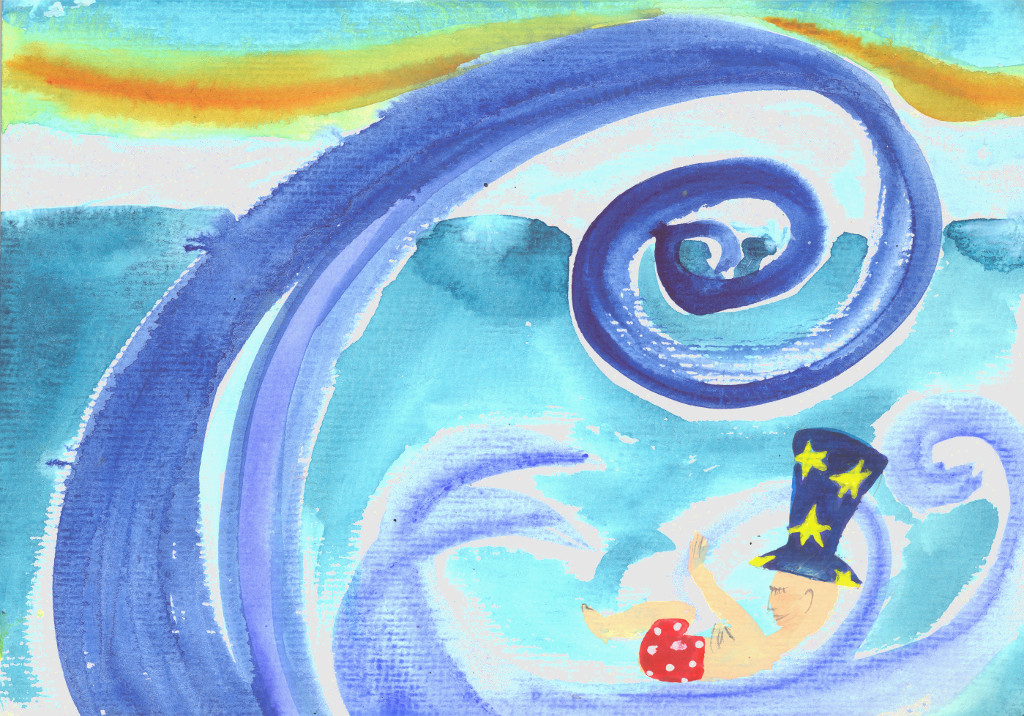
\includegraphics[width=14cm]{Anna4_smj}
					    %\vspace{2cm}
    				} 
                \end{minipage}
                \end{center}
               }
\end{adjustwidth}

\chapter{The basic concepts of quantum mechanics I}

\section{Some linear algebra}
\subsection{Transpose vs. hermitian conjugate}
\lettrine[lines=3,slope=6pt,nindent=6pt]{\initfamily C}{o}nsider a square matrix $A$ with complex numbers $a_{ij}$,
\be
A = \left(\begin{array}{cc}
a_{11} & a_{12} \\
a_{21} & a_{22} 
\end{array} \right)
\ee 
The transpose is changing row to columns:
\be
A^{T} = \left(\begin{array}{cc}
a_{11} & a_{21} \\
a_{12} & a_{22} 
\end{array} \right)
\ee 
The hermitian conjugate is transpose and then complex conjugate and is marked with the "dagger" $^\dag$,
\be
A^{\dag} = \left(\begin{array}{cc}
a_{11}^* & a_{21}^* \\
a_{12}^* & a_{22}^* 
\end{array} \right) 
\ee
Note that for two operators $\hat{A},\hat{B}$,
\be
 \left( AB \right)^\dag = B^\dag A^\dag
\ee
\subsection{Hermitian and unitary operators}
A hermitian operator $\hat{H}$ satisfies
\be
\hat{H} = \hat{H}^\dag  \outnote{Hermitian operator}
\ee
ie. a hermitian operator is its own hermitian conjugate.\nl
\textbf{Theorem:} The eigenvalues of a hermitian operator are always real.\nl
All physical observables are hermitian operators.
A unitary operator $\hat{U}$ satisfies
\be
\hat{U}^{\dag} = \hat{U}^{-1} \outnote{Unitary operator}
\ee
\textbf{Theorem:} A unitary operator doesn't change the norm of a vector.\nl
\textbf{Theorem:} A unitary operator can be written as an exponent of a hermitian operator, 
\be
\hat{U}=e^{i\hat{H}} = \sum_{n=0}^\infty \frac{(i\hat{H})^n}{n!}
\ee

\subsection{Inner product of functions}
The inner (scalar) product of functions $f(x),g(x)$ is defined as
\be
\langle f,g \rangle = \int_{-\infty}^{\infty} f^*(x) g(x) dx \outnote{Scalar product}
\ee
So that the norm squared of a function $\phi(x)$ is simply
\be
\langle \psi, \psi \rangle =  \int_{-\infty}^{\infty} \vert \psi(x) \vert^2 dx
\ee
We see that the "normalization condition" on the wavefunction is that the norm of the wavefunction is equal to one.
\subsection{Delta functions: Dirac vs. Kronecker}
We've defined the Dirac delta function already. The Kronecker delta function $\delta_{ij}$ is defined such that
\be 
\delta_{ij} = \left\{ \begin{array}{cc}
   1 & i=j \outnote{Kronecker delta}\\
   0 & i\ne j
\end{array}\right.
\ee
The orthonormal basis vectors $\phi_i(x)$, $\phi_j(x)$ maintain the inner product relation,
\be  
\langle \phi_i (x) , \phi_j(x) \rangle = \delta_{ij}
\ee
and since they are a basis, it means that any function $\psi(x)$ can be expanded in terms of the basis vectors
\be 
\psi(x) = \sum_i c_i \phi_i(x)
\ee
so that the coefficients $c_i$ can be determined by projecting
\be 
c_i = \langle \phi_i, \psi \rangle = \int_{-\infty}^{\infty} \phi_i^*(x) \psi(x) dx
\ee
And specifically, the norm of $\psi(x)$ is simply
\be 
\langle \psi,\psi \rangle = \sum_i \vert c_i \vert^2
\ee
Which means that a normalized wave-function gives,
\be 
1 = \langle \psi,\psi \rangle = \sum_i \vert c_i \vert^2
\ee
We can swap the order of summation and integration and identify the Dirac delta function, 
\bea 
\psi(x) &=& \sum_i c_i \phi_i(x) \nn
   &=& \sum_i \langle \phi_i, \psi \rangle \phi_i(x) \nn
   &=& \sum_i \left( \int_{-\infty}^{\infty} \phi_i^*(x') \psi(x') dx' \right) \phi_i(x) \nn
   &=& \int_{-\infty}^{\infty} dx'\, \psi(x') \left( \sum_i \phi_i^*(x') \phi_i(x) \right)\nn
   &=& \int_{-\infty}^{\infty} dx'\, \psi(x') \delta(x-x')
\eea
So that, we have the closure relation,
\be
 \delta(x-x') = \sum_i \phi_i^*(x') \phi_i(x) \outnote{Closure relation}
\ee
\subsection{Dual vector spaces / dual basis}
Given any vector space $V$ over $\mathbb{C}$, the dual space $V^*$ is defined as the set of all linear maps $V \rightarrow \mathbb{C}$.

\noindent Given a vector space $V$ with a basis $B$ of vectors indexed as $\vert \phi_i \rangle \in V$, its dual set is a set $B^*$ of vectors $\langle \phi_j \vert \in V^*$ in the dual space $V^*$ such that $B$ and $B^*$ form a biorthogonal system. The dual set is always linearly independent; if it spans $V^*$, then $B^*$ is called the dual basis for the basis $B$.

\noindent For a biorthogonal system, evaluating a dual vector $\langle \phi_j \vert$ on a vector in the original space $\vert \phi_i \rangle$:

\be
\langle \phi_j \vert \phi_i \rangle = \delta_{ij} =
\begin{cases}
  1 & \text{if } i = j\\
  0 & \text{if } i \ne j
\end{cases}
\ee

\section{Dirac bra-ket notation}
We know that a spatial vector $\vec{r}$ can be described in the cartesian basis, eg. $\vec{r} = r_x \vec{e}_x + r_y \vec{e}_y + r_z \vec{e}_z$. But we can also rotate all the axes and then write $\vec{r} = r_x' \vec{e}_{x'} + r_y' \vec{e}_{y'} + r_z' \vec{e}_{z'}$. If we change basis (ie. coordinate system) we need to change the values of the coefficients. But instead of writing the coefficients $(r_x,r_y,r_z)$ or $(r_x',r_y',r_z')$ we can write the vector $\vec{r}$ without referring to the coordinate system (basis). The vector is abstract and needs to be cast in a specified basis to get the "numbers" ie. the coefficients. \nl
In the same way, instead of specifying the quantum state using a wave-function $\psi(x)$ (representation of the quantum state in a specific basis), we can use the \emph{state vector} $\vert \psi \rangle$. The analogy is,
\bea 
(r_x,r_y,r_z) & \longrightarrow & \vec{r} \nn
\psi(\vec{r}) & \longrightarrow &\vert \psi \rangle
\eea
\subsection{Bra and Ket}
A ket vector is the vector representation of a quantum state without specifying the basis. Notice that in
\be
\psi(\vec{r})  \longrightarrow \vert \psi \rangle
\ee
The ket $\vert \psi \rangle$ \emph{doesn't have} $\vec{r}$ in it. This is because $\vec{r}$ is the position basis. $\psi(\vec{r})$ are the components of the abstract ket $\vert \psi \rangle$ in that particular basis: the position basis $\vec{r}$.\nl
The \emph{bra} $\langle \psi \vert $ is a vector in the dual space to the ket space. Formally, it means the bra is a linear functional of the kets. In practice, it is the hermitian conjugate of the ket, so that,
\be 
\langle \psi \vert  = \vert \psi \rangle^\dag
\ee
\subsection{Scalar product}
The scalar product is a complex number and in Dirac notation is written as
\be 
\langle \phi_1 \vert \phi_2 \rangle
\ee
When $\phi_i,\phi_j$ are orthonormal basis vectors then the scalar product is simply the Kronecker delta,
\be 
\langle \phi_i \vert \phi_j \rangle = \delta_{ij}
\ee
Regardless if it operates on basis vectors or on arbitrary vectors, the scalar product obeys the following rules:
\bea 
\langle \phi \vert \psi \rangle &=& \langle \psi \vert \phi \rangle ^* \nn
\langle \phi \vert \lambda_1\psi_1 + \lambda_2\psi_2 \rangle &=& \lambda_1 \langle \phi \vert \psi_1 \rangle + \lambda_2 \langle \phi \vert \psi_2 \rangle \nn
\langle \lambda_1 \phi_1 + \lambda_2 \phi_2 \vert \psi \rangle &=& \lambda_1^* \langle \phi_1 \vert \psi \rangle + \lambda_2^* \langle \phi_2 \vert \psi \rangle \nn
\langle \psi | \psi \rangle & \ge & 0
\eea
\subsection{Projection, projection operators}
Let $\vert \phi_i \rangle$ be an orthonormal basis, $\langle \phi_i \vert \phi_j \rangle = \delta_{ij}$. \nl
Let $\vert\psi\rangle = \sum_i c_i \vert \phi_i \rangle$ be a state vector. Consider the operator $\hat{P}_i$ defined as,
\be
\hat{P}_i = \vert \phi_i \rangle \langle \phi_i \vert \outnote{Projection operator}
\ee
What happens when we operate with $P_i$ on $\vert \psi \rangle$ ?
\bea
\hat{P}_i \vert \psi \rangle &=& \vert \phi_i \rangle \langle \phi_i \vert \sum_j c_j \vert \phi_j \rangle \nn
 &=& \sum_j c_j \vert \phi_i \rangle \langle \phi_i \vert \phi_j \rangle \nn
 &=& \sum_j c_j \vert \phi_i \rangle \delta_{ij} \nn
 &=& c_i \vert \phi_i \rangle
\eea
$\hat{P}_i$ is a \emph{projection operator} that projects any vector it operates on, onto $\phi_i$. Indeed,
\be 
\hat{P}_i^2 = \vert \phi_i \rangle \langle \phi_i \vert \phi_i \rangle \langle \phi_i \vert = \vert \phi_i \rangle \langle \phi_i \vert = \hat{P}_i
\ee 
as we expect from a projection operator. The projector operator is hermitian because
\be 
\hat{P}_i^\dag = \left( \vert \phi_i \rangle \langle \phi_i \vert \right)^\dag = \vert \phi_i \rangle \langle \phi_i \vert = \hat{P}_i
\ee
\subsection{Completeness relation}
Let us start with a geometric example. To describe the $\mathbb{R}^3$ vector space (of real, three dimensional vectors) we need 3 coefficients and a basis. We choose the basis $\vec{e}_x, \vec{e}_y,\vec{e}_z$ so that,
\be
\vec{r} =  x \vec{e}_x + y\vec{e}_y + z\vec{e}_z
\ee
In Dirac notation, this looks like this:
\be 
\vert \vec{r} \rangle = x \vert x \rangle + y \vert y \rangle + z \vert z \rangle
\ee
The \emph{identity operator} $\hat{I}$ does nothing when acting on a vector,
\be 
\hat{I} \vert \vec{r} \rangle = \vert \vec{r} \rangle
\ee
and so does projecting the vector onto all basis components,
\bea
\hat{I} \vert \vec{r} \rangle &=&  \langle x \vert \vec{r} \rangle \vert x \rangle + \langle y \vert \vec{r} \rangle \vert y \rangle + \langle z \vert \vec{r} \rangle \vert z \rangle \nn
 &=&  \left(  \vert x \rangle \langle x \vert+ \vert y \rangle \langle y \vert + \vert z \rangle \langle z \vert \right) \vert \vec{r} \rangle
\eea
In short, the identity operator is the sum of all projections, so for a basis $\vert \phi_i \rangle$, we have,
\be
\hat{I} = \sum_i \vert \phi_i \rangle \langle \phi_i \vert = \sum_i \hat{P}_i \outnote{Completeness relation}
\ee
\subsection{Operators}
An operator $\hat{A}$ operates on a ket $\vert \psi \rangle$ as follows:
\be 
\vert \psi' \rangle = \hat{A} \vert \psi \rangle
\ee
and on a bra,
\be
\langle \psi' \vert  = \langle \psi \vert\hat{A}^{\dag}
\ee
So that, 
\be 
\langle \psi' \vert = \vert \psi' \rangle ^\dag = \left(\hat{A} \vert \psi \rangle \right)^\dag = \langle \psi \vert \hat{A}^\dag
\ee
and,
\bea 
\langle \phi \vert A \vert \psi \rangle &=& \left( A^\dag \vert \phi \rangle \right)^\dag  \vert \psi \rangle \nn
&=& \langle \phi \vert \left( A \vert \psi \rangle \right)
\eea
\textbf{Theorem:} A unitary operator $\hat{U}$ doesn't change the norm of a vector.\nl
\textbf{Proof:} Let $\vert \psi \rangle$ be a normalized vector and $\vert \psi' \rangle = \hat{U} \vert \psi \rangle$. Then
\bea 
\langle \psi' \vert \psi' \rangle = \langle \psi \vert \hat{U}^\dag \hat{U} \vert \psi \rangle = \langle \psi \vert \hat{U}^{-1} \hat{U} \vert \psi \rangle = \langle \psi \vert \psi \rangle
\eea

\section{Physical variables as operators}
Let us summarize what we've learned so far. For a discrete orthonormal basis $\vert \phi_i \rangle$, 
\begin{itemize}
\item Orthonormality: $\langle \phi_i \vert \phi_j \rangle = \delta_{ij}$
\item Closure: $\vert \psi \rangle = \sum_i c_i \vert \phi_i \rangle$
\item Norm squared: $\langle \psi \vert \psi \rangle = \left( \sum_j c_j^* \langle \phi_j \vert \right) \left(  \sum_i c_i \vert \phi_i \rangle \right) = \sum_i \vert c_i \vert ^2$
\item Projection: $c_i = \langle \phi_i \vert \psi \rangle$
\item Completeness: $\hat{I} = \sum_i \vert \phi_i \rangle \langle \phi_i \vert$
\end{itemize}
By analogy, for a continuous orthonormal basis, $\vert x \rangle$, 
\begin{itemize}
\item Orthonormality: $\langle x \vert x' \rangle = \delta(x-x')$
\item Closure: $\vert \psi \rangle = \int_{-\infty}^{\infty} dx\, \psi(x) \vert x \rangle$
\item Norm squared: $\langle \psi \vert \psi \rangle = \left( \int_{-\infty}^{\infty} dx'\, \psi(x')^* \langle x' \vert \right) \left(  \int_{-\infty}^{\infty} dx''\, \psi(x'') \vert x'' \rangle \right) = \int_{-\infty}^{\infty} dx'\, \vert \psi(x') \vert^2$
\item Projection: $\psi(x) = \langle x \vert \psi \rangle$
\item Completeness: $\hat{I} = \int_{-\infty}^{\infty} dx\, \vert x \rangle \langle x \vert$
\end{itemize}
\subsection{Representation of bras and kets}
For a state vector $\vert \psi \rangle = \sum_i c_i \vert \phi_i \rangle$ and a discrete basis $\vert \phi_i \rangle$, we can represent a ket as a column vector,
\be 
\vert \psi \rangle \quad \rightarrow \quad \left( \begin{array}{c}
\langle \phi_1 \vert \psi \rangle \\
\langle \phi_2 \vert \psi \rangle \\
\langle \phi_3 \vert \psi \rangle \\
... \\
\end{array}\right) = 
\left( \begin{array}{c}
c_1 \outnote{"ket"}\\
c_2 \\
c_3 \\
... \\
\end{array}\right)
\ee
Since the bra is the hermitian conjugate of the ket,
\be
\langle \psi \vert = \left( c_1^*, \, c_2^*, \, c_3^*,\, ... \right) \outnote{"bra"}
\ee
The expression for the norm squared is now easy to understand,
\be 
\langle \psi \vert \psi \rangle = \left( c_1^*, \, c_2^*, \, c_3^*,\, ... \right) \left( \begin{array}{c}
c_1 \outnote{bra ket = scalar}\\
c_2 \\
c_3 \\
... \\
\end{array}\right)
 = \sum_i \vert c_i \vert ^2
\ee
The same way, for a state $\vert \psi \rangle = \int dx\, \psi(x) \vert x \rangle$ in the continuous basis $\vert x \rangle$, we have,
\be
\vert \psi  \rangle \rightarrow \left( \begin{array}{c}

\langle x \vert \psi \rangle\\
\downarrow
\end{array} \right) = \left( \begin{array}{c}
\psi(x)\\
\downarrow
\end{array} \right)
\ee
so that its bra is again a hermitian conjugate,
\be
\langle \psi \vert =  \left( \psi^*(x), \quad \rightarrow \right)
\ee
And the norm is,
\be 
\langle \psi \vert \psi \rangle = \left( \psi^*(x), \quad \rightarrow \right) \left( \begin{array}{c}
\psi(x)\\
\downarrow
\end{array} \right)
= \int dx\, \vert \psi(x) \vert^2
\ee
Note that the state can be represented in a different continuous basis, $\vert k \rangle$, so that, $\vert \psi \rangle = \int dk\, \tilde{\psi}(k) \vert k \rangle$
with,
\be
\vert \psi \rangle \rightarrow \left( \begin{array}{c}
\langle k \vert \psi \rangle\\
\downarrow
\end{array} \right) = \left( \begin{array}{c}
\tilde{\psi}(k)\\
\downarrow
\end{array} \right)
\ee
% \textbf{Note:} We see now that the Fourier transform $\tilde{\psi}(k)$ of the wave-function $\psi(x)$ is simply a representation of the same state ket $\vert \psi \rangle$, once in the position basis and once in the wave basis,
% \bea 
% \psi(x) &=& \langle x \vert \psi \rangle \nn
% \tilde{\psi}(k) &=& \langle k \vert \psi \rangle = \int dx\, \langle k \vert x \rangle \langle x \vert \psi \rangle \nn
%   &=& \int dx\, \langle k \vert x \rangle \psi(x) \nn
%   &=& \int dx\, e^{-ikx} \psi(x)
% \eea
% which means that, $\langle k \vert x \rangle = e^{-ikx}$.
\subsection{Representation of operators}
An operator $\hat{A}$ can be represented in the discrete basis $\vert \phi_i \rangle$ as a square matrix,
\be 
\hat{A} \quad \rightarrow \quad \left( \begin{array}{ccccc}
\langle \phi_1 \vert A \vert \phi_1 \rangle & \langle \phi_1 \vert A \vert \phi_2 \rangle & ... & \langle \phi_1 \vert A \vert \phi_j \rangle & ...\\
\langle \phi_2 \vert A \vert \phi_1 \rangle & \langle \phi_2 \vert A \vert \phi_2 \rangle & ... & \langle \phi_2 \vert A \vert \phi_j \rangle & ...\\
...& ... & ... & ...& ...\\
\langle \phi_i \vert A \vert \phi_1 \rangle & \langle \phi_i \vert A \vert \phi_2 \rangle & ... & \langle \phi_i \vert A \vert \phi_j \rangle & ...\\
...& ... & ... & ...& ...
\end{array}\right)
\ee
so that the general element, row $i$ column $j$ is,
\be 
A_{ij} = \langle \phi_i \vert A \vert \phi_j \rangle
\ee
If we have a multiplication of operators $AB$, then the general element is,
\bea
(AB)_{ij} &=&  \langle \phi_i \vert AB \vert \langle \phi_j \rangle \nn
&=& \sum_k \langle \phi_i \vert A \vert \phi_k \rangle \langle \phi_k \vert B \vert \langle \phi_j \rangle \outnote{Operator multiplication}\nn
&=& \sum_k A_{ij} B_{jk} 
\eea
Where we have used the completeness relation going from the first line to the second line. \nl
Now, let $\vert \psi' \rangle = A \vert \psi \rangle$ and $\vert \psi \rangle = \sum_i c_i \vert \phi_i \rangle$, we have,
\bea
\vert \psi' \rangle &=& \sum_i c_i' \vert \phi_i \rangle \nn
c_i' &=& \langle \phi_i \vert \psi' \rangle \nn
   &=& \langle \phi_i \vert A \vert \psi \rangle \nn
   &=& \sum_k \langle \phi_i \vert A \vert \phi_k \rangle \langle \phi_k \vert \psi \rangle \nn
   &=& \sum_k A_{ik} c_k 
\eea
In matrix form,
\be
\left( \begin{array}{c} 
        c_1'\\
        c_2' \\
        ...
       \end{array}
\right) = \hat{A} \left( \begin{array}{c} 
        c_1\\
        c_2 \\
        ...
       \end{array}
\right)
\ee
The hermitian conjugate,
\be
(A^\dag)_{ij} = \langle \phi_i \vert A^\dag \vert \phi_j \rangle = \langle \phi_j \vert A^\dag \vert \phi_i \rangle^* = A_{ji}^*
\ee
We see that taking the hermitian conjugate of $A$ is indeed transposing the then taking the complex conjugate. Therefore, if $A = A^\dag$ then the diagonal elements, $A_{ii} = A_{ii}^*$, meaning that \emph{the diagonal elements of a hermitian matrix are always real numbers}.
% \subsection{Change of basis}
% Let $A$ be an operator and $\hat{U}$ be a unitary operator and let $\vert \phi \rangle = \sum_i c_i \vert \phi_i \rangle$. We define a new basis,
% \be
% \vert \tilde{\phi}_i \rangle = \hat{U} \vert \phi_i \rangle
% \ee
% Now, the operator $\hat{A}$ in the new basis is,
% \bea
% \hat{\tilde{A}}_{ij} &=& \langle \tilde{\phi}_i \vert \hat{A} \vert \tilde{\phi}_j \rangle \nn
%    &=& \langle \phi_i \vert \hat{U}^\dag \hat{A} \hat{U} \vert \phi_j \rangle \nn
%    &=& \left( \hat{U}^{-1} \hat{A} \hat{U} \right)_{ij}\nn
% \hat{\tilde{A}} = \hat{U}^{\dag} \hat{A} \hat{U}
% \eea
% where in the last line we've used $U^{-1} = U^\dag$ which defines a unitary operator.
\subsection{Back to linear polarization}
We now have all the tools to understand the linear polarization of lecture 1. The state of the photons before reaching the polarizer is,
\be
\vert \psi \rangle = \cos \theta \vert \vec{e}_x \rangle + \sin \theta \vert \vec{e}_y \rangle
\ee
The total amplitude of the incoming beam is normalized, so that,
\bea
\langle \psi \vert \psi \rangle &=& \left( \langle \vec{e}_x \vert \cos\theta + \langle \vec{e}_y \vert \sin \theta \right) \left( \cos \theta \vert \vec{e}_x \rangle + \sin \theta \vert \vec{e}_y \rangle\right) \nn
  &=& \cos^2\theta + \sin^2\theta = 1
\eea
The polarizer $\hat{P}_x$ works on this state as is a projection operator to the $x$ axis, giving the state after the polarizer
\be
\vert \psi' \rangle = \hat{P}_x \vert \psi \rangle = \vert \vec{e}_x \rangle \langle \vec{e}_x \vert \psi \rangle = \cos \theta \vert \vec{e}_x \rangle
\ee
so that the probabilityto find a particle after the polarizer is 
\be
\langle \psi' \vert \psi' \rangle = \cos^2 \theta \langle \vec{e}_x \vert \vec{e_x} \rangle = \cos^2 \theta
\ee
which is the classical Malus' law.
\subsection{Momentum and position bases}
Let us define two continuous bases, $\vert x \rangle$ and $\vert p \rangle$. According to our definitions, the orthonormality of the bases is,
\bea
\langle x' \vert x \rangle &=& \delta(x-x') \nn
\langle p' \vert p \rangle &=& \delta(p-p')
\eea
and using the completeness relations, in the $\vert x\rangle $ basis,
\bea
\vert \psi \rangle &=& \int dx\, \vert x\rangle \langle x \vert \psi \rangle \nn
&=& \int dx\, \psi(x) \vert  x \rangle \nn
\psi(x) &=& \langle x \vert \psi \rangle
\eea
whereas in the $\vert p\rangle$ basis,
\bea
\vert \psi \rangle &=& \int dp\, \vert p\rangle \langle p \vert \psi \rangle\nn
&=& \int dp\, \tilde{\psi}(p) \vert p \rangle \nn
\tilde{\psi}(p) &=&  \langle p \vert \psi \rangle 
\eea
What remains is the define the relation between the two bases,
\be
\langle x \vert p \rangle = \frac{1}{2\pi\hbar} e^{ipx/\hbar}
\ee
or in d dimensions,
\be
\langle \vec{x} \vert \vec{p} \rangle = \frac{1}{(2\pi\hbar)^d} e^{i\vec{p}\vec{x}/\hbar}
\ee
So that,
\bea
\psi(x) &=& \langle x \vert \psi \rangle = \langle x \vert \int dx'\,\vert x' \rangle \langle x' \vert \psi \rangle \nn
 &=& \int dx' \langle x \vert x' \rangle \langle x' \vert \psi \rangle \nn
 &=& \int dx' \delta(x-x') \psi(x')
\eea
And also,
\bea
\psi(x) &=& \langle x \vert \psi \rangle = \langle x \vert \int dp\, \vert p \rangle \langle p \vert \psi \rangle \nn
 &=& \int dp \langle x \vert p \rangle \langle p \vert \psi \rangle \nn
 &=& \int dp\, \frac{1}{2\pi\hbar} e^{ipx/\hbar} \langle p \vert \psi \rangle \nn
 &=& \int \frac{dp}{2\pi\hbar}\, e^{ipx/\hbar} \tilde{\psi}(p) \nn
\eea
We see how the Fourier transform is a transform between two bases.
\subsection{Momentum and position operators}
We define the operators $\hat{x},\hat{p}$ so that the basis vectors $\vert x \rangle$ and $\vert p \rangle$ are their eigenvectors, respectively. 
\bea
\hat{x} \vert x_0 \rangle &=& x_0 \vert x_0 \rangle \nn
\hat{p} \vert p_0 \rangle &=& p_0 \vert p_0 \rangle \nn
\eea
These operators are hermitian ($x_0,p_0$ are real numbers), so that,
\bea
\langle x_0 \vert \hat{x} &=& x_0 \langle x_0 \vert\nn
\langle p_0 \vert \hat{p} &=& p_0 \langle p_0 \vert\nn 
\eea
How does the $\hat{p}$ operator act on the state vector $\vert \psi \rangle$ ?
\bea
\label{eq:p_as_derivative}
\langle x \vert \hat{p} \vert \psi \rangle &=& \langle x \vert \hat{p} \vert \int dp\, \vert p \rangle \langle p \vert\psi \rangle \nn
&=& \int dp\, \langle x \vert \hat{p} \vert p \rangle \langle p \vert \psi \rangle \nn
&=& \int dp\, p \langle x \vert p \rangle \langle p \vert \psi \rangle \nn
&=& \int \frac{dp}{2\pi\hbar}\, p e^{ipx/\hbar} \tilde{\psi}(p)\nn
&=& \frac{\hbar}{i} \frac{\partial}{\partial x} \left( \int \frac{dp}{2\pi\hbar}\, e^{ipx/\hbar} \tilde{\psi}(p) \right) \nn
&=& \frac{\hbar}{i} \frac{\partial}{\partial x} \psi(x)\nn
&=& \frac{\hbar}{i} \frac{\partial}{\partial x} \langle x \vert \psi \rangle
\eea
so we can recognize that the momentum operator in the $x$ direction $\hat{p} = \hat{p}_x$, in the ket space, becomes the derivative operator in function space,
\be
\hat{p}_x \rightarrow \frac{\hbar}{i} \frac{\partial}{\partial x}
\ee
or in $d$ dimensions,
\be
\vec{\hat{p}} \rightarrow \frac{\hbar}{i} \vec{\nabla}
\ee
So that the Hamiltonian for a free particle becomes,
\be
\hat{H}_{free} = \frac{\hat{p}^2}{2m} = -\frac{\hbar^2}{2m}\vec{\nabla}^2
\ee
which is familiar from the Schr\"odinger equation.
\subsection{Commutation relations}\
We define the commutator between two operators $\hat{A},\hat{B}$ to be
\be
[\hat{A},\hat{B}] = \hat{A}\hat{B} - \hat{B}\hat{A} = -[\hat{B},\hat{A}] \outnote{Operator commutation}
\ee
Specifically, looking at the operators, $\hat{x},\hat{p}_x$,
\bea
\langle x \vert [\hat{x},\hat{p}_x]\vert\psi\rangle &=& \langle x \vert (\hat{x}\hat{p}_x - \hat{p}_x\hat{x} \vert \psi \rangle  \nn
&=& x \langle x \vert \hat{p}_x \vert \psi \rangle - \frac{\hbar}{i} \frac{\partial}{\partial x} \langle x \vert \hat{x} \vert \psi \rangle \quad \mbox{(Using Eq. \ref{eq:p_as_derivative})} \nn
&=& x \langle x \vert \hat{p}_x \vert \psi \rangle - \frac{\hbar}{i} \frac{\partial x}{\partial x} \langle x \vert \psi \rangle - x \langle x \vert \hat{p}_x \vert \psi \rangle \nn
&=& i\hbar \langle x \vert \psi \rangle
\eea
the above relation holds for any $\vert \psi \rangle$ and so,
\be
[\hat{x},\hat{p}_x] = i\hbar \outnote{Position-momentum commutator}
\ee
Notice that,
\be
[\hat{x},\hat{p}_y] = 0
\ee
Generally,
\be
[\hat{i},\hat{p}_j] = i\hbar \delta_{ij} \quad i,j\in\{x,y,z\}
\ee
\subsection{Sets of commuting variables}
We will discuss three theorems:\nl
\emph{Theorem I}: If two operators $\hat{A},\hat{B}$ commute and if $\vert \psi \rangle$ is an eigenvector of $\hat{A}$, $\hat{B}\vert \psi \rangle$ is also an eigenvector of $\hat{A}$ with the same eigenvalue.\nl
\emph{Proof:} Since $\vert \psi \rangle$ is an eigenvector of $\hat{A}$,
\be
\hat{A} \vert \psi \rangle = a \vert \psi \rangle
\ee
So that,
\be
\hat{B}\hat{A} \vert \psi \rangle = a \hat{B} \vert \psi \rangle
\ee
But $[\hat{A},\hat{B}]=0$ so 
\bea
\hat{B}\hat{A} &=& \hat{A}\hat{B} \nn
\hat{B}\hat{A} \vert \psi \rangle &=& \hat{A}(\hat{B}\vert \psi \rangle) \nn
a (\hat{B} \vert \psi \rangle) &=& \hat{A}(\hat{B}\vert \psi \rangle) 
\eea
\emph{Theorem II}: If two hermitian operators $\hat{A},\hat{B}$ commute and if $\vert a_1 \rangle, \vert a_2 \rangle$ are eigenvectors of $\hat{A}$ with different eigenvalues $a_1,a_2$, then $\langle a_1 \vert \hat{B}\vert a_2 \rangle=0$.\nl
\emph{Proof:} We are told that,
\bea 
\hat{A} \vert a_1 \rangle &=& a_1 \vert a_1 \rangle \nn
\hat{A} \vert a_2 \rangle &=& a_2 \vert a_2 \rangle 
\eea
Since $[\hat{A},\hat{B}]=0$ then
\be 
\langle a_1 \vert \hat{A}\hat{B} - \hat{B}\hat{A} \vert a_2 \rangle = 0
\ee
But, for hermitian $\hat{A}$,
\bea 
\langle a_1 \vert \hat{A}\hat{B} \vert a_2 \rangle &=& a_1 \langle a_1 \vert \hat{B} \vert a_2 \rangle \nn
\langle a_1 \vert \hat{B}\hat{A} \vert a_2 \rangle &=& a_2 \langle a_1 \vert \hat{B} \vert a_2 \rangle 
\eea
So that,
\be
\langle a_1 \vert \hat{A}\hat{B} - \hat{B}\hat{A} \vert a_2 \rangle = (a_1-a_2) \langle a_1 \vert \hat{B} \vert a_2 \rangle= 0
\ee
Since $a_1\ne a_2$ we must have $\langle a_1 \vert \hat{B} \vert a_2 \rangle=0$.\nl
\emph{Theorem III}: If two hermitian operators $\hat{A},\hat{B}$ commute, we can construct an orthonormal basis using eigenvectors common to both of them.

%%%%%%%%%%%%%%%%%%%%%%%%%%%%%%%%%%%%%%%%%%%%%%%%%%%%%%%%%%%%%%%%%%%%%%%%%%%%%%%%%%%%%%%%%
\chapter{The basic concepts of quantum mechanics II}
\section{The Postulates of Quantum Mechanic}
\lettrine[lines=3,slope=6pt,nindent=6pt]{\initfamily W}{e} can now state the postulates of quantum mechanics. We will use them to answer the following questions:
\begin{itemize}
 \item How is the state of a quantum system at a given time described mathematically ?
 \item Given this state, how can we predict the results of the measurements of various physical quantities ?
 \item How can the state of the system at an arbitrary time $t$ be found when the state at time $t_0$ is known ?
\end{itemize}
\subsection{Postulate I:} 
At a fixed time $t_0$, the state of the system is defined by specifying a ket $\vert \psi(t_0) \rangle$\nl
Since $\vert \psi(t_0) \rangle$ belongs to a linear vector space, a linear combination of state vectors is also a state vector.  
\subsection{Postulate II:} 
Every measurable quantity $A$ can be described by an operator $\hat{A}$. This operator is an observable.\nl
Unlike classical mechanics, the state is represented by a vector and a physical quantity is represented by an operator.
\subsection{Postulate III:} 
The only possible result of a measurement of a physical quantity $A$ is one of the eigenvalues of the corresponding observable $\hat{A}$.

\noindent The measurement of $A$ always gives a real number because $A$ is by definition hermitian.

\noindent If the spectrum of $A$ is discrete, the results that can be obtained when measuring $A$ are quantized.
%
\subsection{Postulate IV: (discrete non-degenerate spectrum)}
Consider a normalized quantum state $\vert \psi \rangle$ so that $\langle \psi \vert \psi \rangle = 1$.\nl
Let $\vert \phi_n \rangle$ be the normalized eigenvectors of $A$ such that, $A \vert \phi_n \rangle = A_n \vert \phi_n \rangle$.\nl
The probability of measuring a non-degenerate value $A_n$ of $A$ is
\be
P(A_n) = \left\vert \langle \phi_n \vert \psi \rangle \right\vert ^2
\ee
As a consequence, if $\vert \psi' \rangle = e^{i\theta} \vert \psi \rangle$ then,
\bea 
\langle \psi' \vert \psi' \rangle &=& \langle \psi \vert e^{-i\theta}e^{i\theta} \vert \psi \rangle = 1 \nn
P(A_n) &=& \left\vert \langle \phi_n \vert \psi \rangle \right\vert^2  \nn
  &=& \left\vert \langle \phi_n \vert \psi ' \rangle e^{-i\theta} \right \vert ^2
\eea
Therefore, multiplying the state vector by a constant phase doesn't change the physical result. The generalization to a continuous spectrum is quite simple.
\subsection{Postulate V:}
If the measurement of a physical quantity $\hat{A}$ on the system in the state $\vert \psi \rangle$ gives the result $A_n$, the state of the system immediately after the measurement is the normalized projection $\vert \psi'\rangle$ ,
\be 
\vert \psi'\rangle = \frac{\hat{P}_n \vert \psi \rangle}{\sqrt{\langle \psi \vert \hat{P}_n \vert \psi \rangle}}
\ee
Previously, we saw the example of the linear polarizer. The quantum state before the polarizer is $\vert \psi \rangle$ which in that example is a superposition of two states. The forth postulate allows us to predict the probabilities of obtaining the possible results. But when the measurement is actually performed, only one of the possible results is obtained. Immediately after this measurement, there is no sense of talking about the probability of obtaining a value: we already know which value was obtained: information was transferred from the system to us - the "observer". The fact that information has passed out of the "system" to the "observer", means that the quantum state after the measurement has to be different. It is no longer a superposition of states but only the state that was measured. This is sometimes called "collapse of the wave-function" and is a subject of endless philosophical and new-age debate.
\subsection{Postulate VI:}
The time evolution of the state vector $\vert \psi(t) \rangle$ is governed by the Schr{\"o}dinger equation,
\be
i\hbar \frac{d}{dt}\vert \psi(t) \rangle = \hat{H}(t)\vert \psi(t) \rangle 
\label{eq:shr_postulate}
\ee
Where $\hat{H}$ is the Hamiltonian operator and is the observable associated with the total energy of the system.
\section{Hamiltonian}
We have seen that moving from classical mechanics to quantum mechanics means changing the variables $x,p$ with operators $\hat{x},\hat{p}$ which have nontrivial commutation relations.
In our course, we will only consider time-independent Hamiltonians of the form,
\be
\hat{H} = \frac{\hat{p}^2}{2m} + V(\hat{x})
\ee
and the time evolution of the state ket is,
\be
\hat{H} \vert \psi(t) \rangle = \left(\frac{\hat{p}^2}{2m} + V(\hat{x}) \right)\vert \psi(t) \rangle
\ee
We've seen that,
\be
\hat{p} \rightarrow -i\hbar \vec{\nabla}
\ee
and that,
\be 
\langle x \vert V(\hat{x}) \vert \psi(t) \rangle \rightarrow V(x)\psi(x,t)
\ee
so that
\be
\langle x \vert \hat{H}\vert \psi(t) \rangle = -\frac{\hbar^2}{2m}\nabla^2 \langle x \vert \psi(t) \rangle + \langle x \vert V(\hat{x}) \vert \psi(t) \rangle
\ee
And the Schr{\"o}dinger equation, Eq. \ref{eq:shr_postulate}, becomes its now familiar form to us,
\be 
i\hbar \frac{\partial}{\partial t}\psi(x,t) = \left( -\frac{\hbar^2}{2m}\nabla^2 + V(x) \right) \psi(x,t)
\ee
\subsection{Expectation value of the Hamiltonian}
Let $\vert \phi_n \rangle$ be an eigenstate of the Hamiltonian such that,
\be 
\hat{H} \vert \phi_n \rangle = E_n \vert \phi_n \rangle
\ee
The let the state $\vert \psi \rangle = \sum_n c_n \vert \phi_n \rangle$. \nl
The expectation value of the Hamiltonian in this state is,
\bea
\langle \psi \vert \hat{H} \vert \psi \rangle &=& \sum_{nm} c_m^* c_n \langle \phi_m \vert \hat{H} \vert \phi_n \rangle \nn
   &=& \sum_{nm} c_m^* c_n E_n \langle \phi_m \vert \phi_n \rangle \nn
   &=& \sum_{nm} c_m^* c_n E_n \delta_{nm} \nn
   &=& \sum_{n} \vert c_n\vert^2 E_n \nn
   &=& \sum_{n} P(n) E_n 
\eea
Where $\vert c_n\vert^2=P(n)$ is the probability to find the system in state $n$. So we see that the expectation value of the Hamiltonian is the total energy of the system.
\subsection{Unitary evolution}
Let $\vert \phi_n \rangle$ be an eigenstate of the Hamiltonian such that,
\be 
\hat{H} \vert \phi_n(t) \rangle = E_n \vert \phi_n(t) \rangle
\ee
The Schr{\"o}dinger equation \ref{eq:shr_postulate} tells us that,
\bea
i\hbar\frac{d}{dt}\vert \phi_n(t) \rangle &=& \hat{H}\vert \phi_n(t) \rangle \nn
 &=& E_n \vert \phi_n(t) \rangle \nn
\vert \phi_n(t) \rangle &=& e^{-i\hat{H} t/\hbar}\vert \phi_n(t=0) \rangle \equiv e^{-iE_n t/\hbar}\vert \phi_n \rangle
\eea
We see that the unitary operator $\hat{U}(t)\equiv e^{-i\hat{H} t/\hbar}$ gives the time evolution of the system. Specifically, for 
\bea
\vert \psi(t=0) \rangle &=& \sum_n c_n \vert \phi_n \rangle \nn
\vert \psi(t) \rangle &=&  e^{-i\hat{H} t/\hbar} \vert \psi(0) \rangle \nn
 &=& \sum_n c_n e^{-i\hat{H} t/\hbar} \vert \phi_n \rangle \nn
 &=& \sum_n c_n e^{-i E_n t/\hbar} \vert \phi_n \rangle
\eea
so that the probability to find the system in a certain eigenstate (stationary state) $\vert m\rangle $ at time $t$ doesn't change with time,
\bea 
P(m) &=& \left\vert \langle \phi_m \vert \psi(t) \rangle \right\vert^2 \nn
&=& \left\vert \sum_n c_n e^{i E_n t/\hbar}  \langle \phi_m \vert \phi_n \rangle \right\vert^2 \nn
&=& \left\vert e^{i E_m t/\hbar} c_m \right\vert^2 \nn
&=& \left\vert c_m \right\vert^2
\eea
But the probability to find the system in its initial state at time $t$ can change,
\bea 
P(t) &=& \left\vert \langle \psi(t=0) \vert \psi(t) \rangle \right\vert^2 \nn
&=& \left\vert \left(\sum_m \langle \phi_m\vert c_m^* \right) \left( \sum_n  c_n e^{i E_n t/\hbar} \vert \phi_n \rangle\right) \right\vert^2 \outnote{Probability to find the system in its initial state}\nn
&=& \left\vert \sum_n \vert c_n \vert^2 e^{i E_n t/\hbar} \right\vert^2 \ne \left\vert \sum_n \vert c_n \vert^2 \right\vert ^2
\eea
\section{Expectation value}
The result of a measurement of an observable $\hat{A}$ on the state $\vert \psi(t) \rangle$ is the ``sandwich'',
\be 
\langle \psi(t) \vert \hat{A} \vert \psi(t) \rangle \equiv \langle A \rangle (t)
\ee
It means that: measure many times identical systems, each system in the same state $\vert \psi(t) \rangle$.\nl
Notice that, for $\hat{A} \vert \phi_n \rangle = a_n \vert \phi_n \rangle$ we have,
\bea
\langle \psi \vert \hat {A} \vert \psi \rangle &=& \sum_n \langle \psi \vert \hat{A} \vert \phi_n \rangle \langle \phi_n \vert \psi \rangle \nn
  &=& \sum_n a_n \langle \psi \vert \phi_n \rangle \langle \phi_n \vert \psi \rangle \nn
  &=& \sum_n a_n \left\vert \langle \phi_n \vert \psi \rangle \right\vert^2 \nn
  &=& \sum_n a_n P(n) \nn
\eea
with $P(n)$ the probability to find the system in state $n$. We see that $\langle \psi \vert \hat{A} \vert \psi \rangle$ is indeed the mean value of the observable $\hat{A}$ as defined in probability theory.\nl
Notice that in general, if we know the wavefunction $\psi(x) = \langle x \vert \psi \rangle$ we can always calculate an expectation value of an operator $\hat{A}$ using the position basis,
\be
\langle \psi \vert \hat{A} \vert \psi \rangle = \int dx'\, \int dx'' \, \langle \psi\vert x' \rangle \langle x' \vert \hat{A} \vert x'' \rangle \langle x'' \vert \psi \rangle
\ee
and in particular, if it is a function of $\hat{x}$, ie. $\hat{A} = A(\hat{x})$, then 
\bea 
\hat{A} \vert x' \rangle &=& A(x') \vert x' \rangle \nn
\langle x'' \vert \hat{A} \vert x' \rangle &=& A(x') \langle x'' \vert x' \rangle \nn
 &=& A(x') \delta(x'-x'')\nn
\langle \psi \vert \hat{A} \vert \psi \rangle &=& \int dx'\, \int dx'' \, \langle \psi\vert x' \rangle \langle x' \vert \hat{A} \vert x'' \rangle \langle x'' \vert \psi \rangle \nn
   &=& \int dx'\, \int dx'' \, \langle \psi\vert x' \rangle A(x')\delta(x'-x'') \langle x'' \vert \psi \rangle \nn
   &=& \int dx'\, \langle \psi\vert x' \rangle A(x') \langle x' \vert \psi \rangle \nn 
   &=& \int dx'\, \psi^*(x') A(x') \psi(x')
\eea

\subsection{Ehrenfest's Theorem}
Let us look at the time evolution of the observed value of $\hat{A}$
\be
\frac{d}{dt} \langle \psi(t) \vert \hat{A} \vert \psi(t) \rangle = \left( \frac{d}{dt}  \langle \psi(t) \vert \right) \hat{A} \vert \psi(t) \rangle+ \langle \psi(t) \vert \hat{A} \left( \frac{d}{dt} \vert \psi(t) \rangle\right) 
\ee
But,
\bea 
\frac{d}{dt}\vert \psi(t) \rangle &=& \frac{1}{i\hbar} \hat{H} \vert \psi(t) \rangle \nn
\frac{d}{dt}\langle \psi(t) \vert &=& -\frac{1}{i\hbar} \hat{H} \langle \psi(t) \vert 
\eea
So we get,
\bea 
\frac{d}{dt} \langle \psi(t) \vert \hat{A} \vert \psi(t) \rangle &=& \frac{1}{i\hbar} \langle \psi(t) \vert \hat{A}\hat{H}-\hat{H}\hat{A} \vert \psi(t) \rangle  \outnote{Ehrenfest's Theorem}\nn
 \frac{d}{dt} \langle \hat{A} \rangle &=& \frac{1}{i\hbar}\langle [\hat{A},\hat{H}] \rangle
\eea
The result above is called Ehrenfest's theorem and it states that the change in time of an observed quantity $\langle A \rangle$ is related to the expectation value of its commutator with the Hamiltonian. Therefore, if an operator $\hat{A}$ commutes with the Hamiltonian, its expectation value $\langle \hat{A} \rangle$ doesn't change with time (and is called a constant of motion). You can now see why when the Hamiltonian doesn't depend on time, then the energy of the system is constant,
\bea 
E &=& \langle \hat{H} \rangle \nn
\frac{dE}{dt} &=& \frac{1}{i\hbar}\langle [\hat{H},\hat{H}] \rangle = 0 \nn
E &=& const
\eea
Let's look at two special observables, $\hat{x},\hat{p}$.\nl
Let the Hamiltonian be $\hat{H} = \frac{\hat{p}^2}{2m} + V(\hat{x})$, Ehrenfest's theorem tells us that, 
\bea 
\frac{d\langle \hat{x} \rangle}{dt} &=& \frac{1}{i\hbar}\langle[\hat{x},\hat{H} ]\rangle \nn
 &=& \frac{1}{i\hbar}\langle[\hat{x},\frac{\hat{p}^2}{2m} ]\rangle  + \frac{1}{i\hbar}\langle[\hat{x},V(\hat{x}) ]\rangle \nn
 &=& \frac{1}{i\hbar}\langle[\hat{x},\frac{\hat{p}^2}{2m} ]\rangle \nn 
 &=& \frac{1}{i\hbar} \langle\frac{i\hbar}{m}\hat{p}\rangle \outnote{Classical correspondence: velocity} \nn 
\frac{d\langle \hat{x} \rangle}{dt} &=& \frac{\langle \hat{p} \rangle}{m} 
\eea
And,
\bea 
\frac{d\langle \hat{p} \rangle}{dt} &=& \frac{1}{i\hbar}\langle[\hat{p},\hat{H} ]\rangle \nn
 &=& \frac{1}{i\hbar}\langle[\hat{p},\frac{\hat{p}^2}{2m} ]\rangle  + \frac{1}{i\hbar}\langle[\hat{p},V(\hat{x}) ]\rangle \nn
 &=& \frac{1}{i\hbar}\langle[\hat{p},V(\hat{x}) ]\rangle \nn
 &=& \frac{1}{i\hbar} \langle-i\hbar \frac{d}{dx}V(\hat{x})\rangle \outnote{Classical correspondence: force}\nn 
\frac{d\langle \hat{p} \rangle}{dt} &=& -\frac{\langle \frac{d}{dx}V(\hat{x}) \rangle}{m} 
\eea
We see that the expectation values of $\hat{x},\hat{p}$ evolve like in classical mechanics !
\subsection{Standard deviation and uncertainty}
We define the deviation of an observable $\hat{A}$ from its expectation value $\langle \hat{A} \rangle$ as,
\be
(\Delta A)^2 = \left\langle \psi \left\vert \left(\hat{A} - \langle \hat{A} \rangle\right)^2 \right\vert \psi \right\rangle = \langle \hat{A}^2 \rangle - \langle \hat{A} \rangle^2 \ge 0
\ee
it is easy to verify that the quantity above is always positive. The root-mean-square (RMS) deviation is simply,
\be
\Delta A = \sqrt{(\Delta A)^2} = \sqrt{\langle \hat{A}^2 \rangle - \langle \hat{A} \rangle^2}
\ee
(Note: for Gaussian distribution this is the width of the Gaussian).\nl
We define the operator $\hat{B}$ and the state $\vert \phi \rangle$ such that,
\bea 
\hat{B} &=& \left(\hat{x}  + i\lambda \hat{p}\right) \nn
\lambda &>&0 \nn
\vert \phi \rangle &=& \hat{B} \vert \psi \rangle = \left(\hat{x}  + i\lambda \hat{p}\right) \vert \psi \rangle
\eea
with a positive norm,
\bea
\langle \phi \vert \phi \rangle &=& \langle \psi \vert B^\dag B \vert \psi \rangle \ge 0\nn
\langle \phi \vert \phi \rangle &=& \langle \psi \vert \left(\hat{x}  - i\lambda \hat{p}\right)\left(\hat{x}  + i\lambda \hat{p}\right)\vert \psi \rangle \ge 0\nn
 &=& \langle \psi \vert\hat{x}^2  \vert \psi \rangle + \langle \psi \vert i\lambda \left(\hat{x}\hat{p}  - \hat{p}\hat{x}\right)\vert \psi \rangle + \langle \psi \vert \lambda^2 \hat{p}^2\vert \psi \rangle \ge 0 \nn
 &=& \langle \hat{x}^2 \rangle + i\lambda \langle [\hat{x},\hat{p}] \rangle + \lambda^2 \langle \hat{p}^2 \rangle \ge 0\nn
 &=& \langle \hat{x}^2 \rangle -\hbar \lambda + \lambda^2 \langle \hat{p}^2 \rangle \ge 0
\eea
The above is a quadratic equation in $\lambda$ which is always positive which means that the discriminant is negative or zero,
\bea 
\hbar^2 - 4 \langle \hat{p}^2 \rangle \langle \hat{x}^2 \rangle &\le& 0 \nn
\langle \hat{p}^2 \rangle \langle \hat{x}^2 \rangle \ge \frac{\hbar^2}{4}
\label{eq:rms_xp}
\eea
Next, we can define the operators,
\bea
\hat{\Delta p} &=& \hat{p} - \langle \hat{p} \rangle \nn
\hat{\Delta x} &=& \hat{x} - \langle \hat{x} \rangle \nn
\eea
Notice that the commutation relation stays the same,
\be
[\hat{\Delta x},\hat{\Delta p}] = [\hat{x},\hat{p}] = i\hbar 
\ee
So that, according to this and equation Eq. \ref{eq:rms_xp}, we have,
\be
\langle \hat{\Delta p}^2 \rangle \langle \hat{\Delta x}^2 \rangle \ge \frac{\hbar^2}{4}
\ee
and together with the RMS value $\Delta p = \sqrt{\langle \hat{\Delta p}^2}$ etc.,
\be
\Delta p \Delta x = \sqrt{\langle \hat{\Delta p}^2 \rangle } \sqrt{\langle\hat{\Delta x}^2 \rangle} \ge \frac{\hbar}{2} \outnote{Heisenberg's uncertainty principle}
\ee
So we have proved the uncertainty relation between the observables $\hat{x},\hat{p}$ rigorously! Notice that this worked because
\be
[\hat{x},\hat{p}] = i\hbar
\ee
so we conclude that it works for any two observables that have this commutation relation. Conversely, commuting observables (say $\hat{x}$, $\hat{p}_y$) do not have this relation.
\section{Site system, position, translation}
Consider a system with only three sites, such that one way to describe the system is using the position basis $\vert 0\rangle,\vert 1\rangle,\vert 2\rangle$. This means that an arbitrary state of the system is,
\be
\vert \psi \rangle = c_0 \vert 0 \rangle  + c_1 \vert 1 \rangle + c_2 \vert 2 \rangle
\ee
%\begin{figure}[!ht]
%  \centering
%  \includegraphics[width=10cm]{three_sites.pdf}\\
%  \caption{Schematic of a three site system with periodic boundary conditions}
%  \label{fig:three_sites}
%\end{figure}
Or in vector notation, the basis is
\be
\vert 0 \rangle \rightarrow \left(\begin{array}{c}
                                   1\\
                                   0\\
                                   0\\		    
                                  \end{array}
 \right) \quad ; \quad 
\vert 1 \rangle \rightarrow \left(\begin{array}{c}
                                   0\\
                                   1\\
                                   0\\		    
                                  \end{array}
 \right) \quad ; \quad 
\vert 2 \rangle \rightarrow \left(\begin{array}{c}
                                   0\\
                                   0\\
                                   1\\		    
                                  \end{array}
 \right) 
\ee
The above basis is the position basis, so that it is the eigenbasis of the position operator,
\be
\hat{x} \vert 0 \rangle = 0 \vert 0 \rangle \quad ; \quad \hat{x} \vert 1 \rangle = 1 \vert 1 \rangle \quad ; \quad \hat{x} \vert 2 \rangle = 2 \vert 2 \rangle  
\ee
So that, in this basis, we can represent the position operator as a matrix,
\be 
\hat{x} \rightarrow \left( \begin{array}{ccc}
                            0 & 0 & 0 \\
                            0 & 1 & 0 \\
                            0 & 0 & 2 
                           \end{array}
\right)
\ee
It is easy to check that this is true, eg.,
\be
\hat{x} \vert 2 \rangle = 2 \vert 2 \rangle \rightarrow  \left( \begin{array}{ccc}
                            0 & 0 & 0 \\
                            0 & 1 & 0 \\
                            0 & 0 & 2 
                           \end{array}
\right) \left(\begin{array}{c}
                                   0\\
                                   0\\
                                   1\\		    
                                  \end{array}
 \right) = 2 \left(\begin{array}{c}
                                   0\\
                                   0\\
                                   1\\		    
                                  \end{array}
 \right)
\ee
We can also define the translation operator $\hat{D}$ such that,
\be
\hat{D}\vert i \rangle = \vert i-1\rangle \outnote{Translation operator}
\ee
eg. $\hat{D}\vert 2 \rangle = \vert 1 \rangle$. Which means that without periodic boundary conditions, $\hat{D}\vert 1 \rangle = \vert 0\rangle $ and $\hat{D}\vert 0 \rangle = 0 $ and generally, in the position basis, we have
\be
\label{eq:D_operator}
\hat{D} \rightarrow \left( \begin{array}{ccc}
                            0 & 1 & 0 \\
                            0 & 0 & 1 \\
                            0 & 0 & 0 
                           \end{array}
\right)
\ee
Which means that $\hat{D}\vert 0 \rangle = 0$.\nl
Notice that it is not hermitian. Its hermitian conjugate is
\be
\hat{D}^\dag \vert i \rangle = \vert i+1 \rangle
\ee
which can be seen from its hermitian conjugate in the position basis,
\be
\hat{D}^\dag  \rightarrow \left( \begin{array}{ccc}
                            0 & 0 & 0 \\
                            1 & 0 & 0 \\
                            0 & 1 & 0 
                           \end{array}
\right)
\ee
Notice the commutation relation,
\bea
[\hat{D},\hat{x}]\vert n \rangle &=& (\hat{D}\hat{x} - \hat{x}\hat{D})\vert n \rangle \nn
   &=& \hat{D}n\vert n \rangle - \hat{x}\vert n-1 \rangle \nn
   &=& n\vert n-1 \rangle - (n-1)\vert n-1 \rangle \nn
   &=& \vert n-1 \rangle = \hat{D} \vert n \rangle
\eea
The above is true for any ket $\vert n \rangle$, so that
\bea
\label{eq:Dx_commutation}
[\hat{D},\hat{x}] &=& \hat{D} \nn
[\hat{D}^\dag,\hat{x}] &=& -\hat{D}^\dag \nn
\eea
We say that $\hat{D}$ is a lowering operator on $\hat{x}$ and that $\hat{D}^\dag$ a raising operator. That is because operating with them on the eigenstates of $\hat{x}$ lowers/raises the value of $\hat{x}$ by one. We will see similar operators we study the harmonic oscillator.
% We can define the momentum basis as the discrete Fourier transform of the position basis, with the discrete momenta as $k_n = \frac{2\pi}{3}n$
% \bea
% \vert k \rangle &=& \frac{1}{\sqrt{N}} \sum_x e^{ikx} \vert x \rangle \nn
% \vert k =0 \rangle &=& \frac{1}{\sqrt{3}} (\vert 1 \rangle + \vert 2 \rangle + \vert 3 \rangle)\rangle \nn
% \vert k =\frac{2\pi}{3} \rangle &=& \frac{1}{\sqrt{3}} (e^{i\frac{2\pi}{3}}\vert 1 \rangle + e^{i\frac{4\pi}{3}}\vert 2 \rangle + e^{i\frac{6\pi}{3}}\vert 3 \rangle)\rangle \nn
%      &=& \frac{1}{\sqrt{3}} (e^{i\frac{2\pi}{3}}\vert 1 \rangle + e^{i\frac{4\pi}{3}}\vert 2 \rangle + \vert 3 \rangle)\rangle \nn
% \vert k =\frac{4\pi}{3} \rangle &=& \frac{1}{\sqrt{3}} (e^{i\frac{4\pi}{3}}\vert 1 \rangle + e^{i\frac{8\pi}{3}}\vert 2 \rangle + e^{i\frac{12\pi}{3}}\vert 3 \rangle)\rangle \nn
%      &=& \frac{1}{\sqrt{3}} (e^{i\frac{4\pi}{3}}\vert 1 \rangle + e^{i\frac{2\pi}{3}}\vert 2 \rangle + \vert 3 \rangle)\rangle 
% \eea
% Notice that $k=-\frac{2\pi}{3}$ and $k=\frac{4\pi}{3}$ are the same. \nl
% The momentum basis is the eigenbasis of the momentum operator,
% \be
% \hat{p} \vert k \rangle = \hbar k \vert k \rangle
% \ee
% So that in the position basis,
% \be
% \langle i \vert \hat{p} \vert \j \rangle 
% \ee


%%%%%%%%%%%%%%%%%%%%%%%%%%%%%%%%%%%%%%%%%%%%%%%%%%%%%%%%%%%%%%%%%%%%%%%%%%%%%%%%%%%%%%%%%

\chapter{Harmonic Oscillator}
\section{Classical oscillator}
\lettrine[lines=3,slope=6pt,nindent=6pt]{\initfamily W}{e} are well familiar with the classical harmonic oscillator, the potential energy is
\be 
V(x) = \frac{1}{2}k x^2 = \frac{1}{2}m\omega^2 x^2 \outnote{Harmonic potential}
\ee
so that the force pulling back to the center is Fick's law,
\be 
f = -\frac{dV}{dx} = -kx
\ee
with a frequency,
\be 
\omega = \sqrt{\frac{k}{m}}
\ee
It has numerous uses, eg.
\begin{itemize}
\item Is is one of the few exactly solvable models.
\item Near a potential minimum, every potential can be approximated as a harmonic oscillator (Taylor expand to leading order).
\item It can model the movement of atoms in a lattice.
\item It can model the vibrations of the electromagnetic field.
\end{itemize}
We identify the total energy of the oscillator as the sum of the kinetic and the potential terms. This is the Hamiltonian,
\be 
H = \frac{p^2}{2m} + \frac{1}{2}m \omega^2 x^2 \outnote{Harmonic oscillator Hamiltonian}
\ee
\section{Quantum harmonic oscillator in one dimension}
\subsection{Quantization}
When changing from classical mechanics to quantum mechanics we substitute the variables to operators, $x\rightarrow \hat{x}$ and $p\rightarrow \hat{p}$. The Hamiltonian is an operator,
\be 
\hat{H} = \frac{\hat{p}^2}{2m} + \frac{1}{2}m \omega^2 \hat{x}^2
\ee
we recall that:
\begin{itemize}
\item The commutation relation, $[\hat{x},\hat{p}] = i\hbar$.
\item The expectation value of the Hamiltonian is the total energy $E = \langle \hat{H} \rangle.$
\item Since the Hamiltonian doesn't depend on time, the total energy doesn't depend on time, so we can solve the time-independent Schodinger equation $\hat{H} \vert \phi_n \rangle = E_n \vert \phi_n \rangle$ to get the stationary states $\vert \phi_n \rangle$ and their energy spectrum $E_n$.
\item In the position basis, we change the operator $\hat{p} \rightarrow -i\hbar \frac{\partial}{\partial x}$.
\end{itemize}
So the problem reduces to the usual eigenvalue problem,
\be
\hat{H} \vert \phi_n \rangle = E_n \vert \phi_n \rangle \quad\,\,\,\, n=0,1,2,... \outnote{Energy basis}
\ee
With the solutions an orthonormal basis,
\be
\langle \phi_n \vert \phi_m \rangle = \delta_{nm} 
\ee
\subsection{Wavefunctions}
To find the wavefunctions in the position basis, we solve the differential equation which is the time-independent Schr{\"o}dinger equation,
\bea
\phi_n(x) &=& \langle x \vert \phi_n \rangle \nn
\left(-\frac{\hbar^2}{2m}\frac{d^2}{dx^2} + \frac{1}{2}m\omega^2 x^2\right) \phi_n(x) &=& E_n \phi_n(x)
\eea
The solutions are the stationary states of the harmonic oscillator, they are the \href{http://en.wikipedia.org/wiki/Hermite_polynomials}{Hermite polynomials}. Here are the first three,
\bea
\phi_0(x) &=& \left(\frac{m\omega}{\pi\hbar}\right)^{1/4} e^{-\frac{1}{2}\frac{m\omega}{\hbar}x^2}\nn
\phi_1(x) &=& \sqrt{2\pi}\left(\frac{m\omega}{\pi\hbar}\right)^{3/4} x e^{-\frac{1}{2}\frac{m\omega}{\hbar}x^2} \outnote{First 3 oscillator wave-functions}\nn
\phi_2(x) &=& \left(\frac{m\omega}{4\pi\hbar}\right)^{1/4} \left(2\frac{m\omega}{\hbar}x^2-1\right) e^{-\frac{1}{2}\frac{m\omega}{\hbar}x^2}
\eea
with the property that for $\phi_n(x)$, if $n=2m$ is even, there are only even powers of $x^{2m},x^{2m-2},...$ and if $n=2m+1$ is odd, there are only odd powers of $x^{2m+1},x^{2m-1},...$. This symmetry has important implications for expectation values, ie,
\bea 
\langle \phi_n \vert \hat{x} \vert \phi_n \rangle &=& 0 \outnote{Orthogonality}\nn
\langle \phi_n \vert \hat{x}^2 \vert \phi_n \rangle &\neq & 0 
\eea
so that the mean potential and kinetic energy in a given state $\vert \phi_n \rangle$ are,
\bea
\left\langle \phi_n \left\vert \frac{1}{2}m\omega^2 \hat{x}^2 \right\vert \phi_n \right\rangle &=& \frac{1}{2}m\omega^2 \int_{-\infty}^{\infty} dx\, \vert\phi_n(x)\vert^2 x^2 \nn
\left\langle \phi_n \left\vert \frac{\hat{p}^2}{2m} \right\vert \phi_n \right\rangle &=& -\frac{\hbar^2}{2m} \int_{-\infty}^{\infty} dx\, \phi_n^*(x) \frac{d^2}{dx^2} \phi_n(x)
\eea
\section{Raising or lowering operators}
\subsection{Definition}
We define the lowering (destruction) and raising (creation) operators,
\bea 
\hat{a} &=& \sqrt{\frac{m\omega}{2\hbar}}\left(\hat{x} + \frac{i}{m\omega}\hat{p} \right) \outnote{Lowering/raising operators}\nn
\hat{a}^\dag &=& \sqrt{\frac{m\omega}{2\hbar}}\left(\hat{x} - \frac{i}{m\omega}\hat{p} \right)
\eea
So that,
\bea
\hat{x} &=& \sqrt{\frac{\hbar}{2m\omega}}(\hat{a}^\dag+\hat{a})\nn
\hat{p} &=& i\sqrt{\frac{ m\omega\hbar}{2}}(\hat{a}^\dag-\hat{a})
\eea
and the commutation,
\bea 
[\hat{x},\hat{p}] &=& i\hbar \nn
\frac{i\hbar}{2}\left[\hat{a}^\dag+\hat{a}, \hat{a}^\dag-\hat{a}\right] &=& i\hbar \nn
-[\hat{a}^\dag,\hat{a}] + [\hat{a},\hat{a}^\dag] &=& 2 \nn
[\hat{a},\hat{a}^\dag] &=& 1
\eea
Looking at the last line we see that,
\bea
\label{eq:osc_commutation} 
\hat{a}\hat{a}^\dag - \hat{a}^\dag\hat{a} &=& 1 \nn
\hat{a}\hat{a}^\dag &=& \hat{a}^\dag\hat{a} + 1
\eea
\subsection{Hamiltonian}
Now we see that,
\bea
\frac{\hat{p}^2}{2m} &=& -\frac{\hbar\omega}{4}(\hat{a}^\dag-\hat{a})^2 \nn
           &=& -\frac{\hbar\omega}{4}\left((\hat{a}^\dag)^2 + \hat{a}^2 - \hat{a}^\dag\hat{a} - \hat{a}\hat{a}^\dag\right) \nn
\frac{1}{2}m \omega^2 \hat{x}^2 &=& \frac{\hbar\omega}{4} (\hat{a}^\dag+\hat{a})^2 \nn
           &=& \frac{\hbar\omega}{4} \left((\hat{a}^\dag)^2+\hat{a}^2+ \hat{a}^\dag\hat{a} + \hat{a}\hat{a}^\dag\right) \nn 
 \hat{H} &=& \frac{\hat{p}^2}{2m} +\frac{1}{2}m \omega^2 \hat{x}^2 \nn
   &=& \frac{\hbar \omega}{2}\left( \hat{a}^\dag\hat{a} + \hat{a}\hat{a}^\dag \right) \nn
   &=& \hbar \omega\left( \hat{a}^\dag\hat{a} + \frac{1}{2} \right) 
\eea
Where in the last line we've used the oscillator commutation relations, Eq. \ref{eq:osc_commutation}. So we have reached the important conclusion, that in terms of the raising $\hat{a}^\dag$ and lowering $\hat{a}$ operators, the harmonic oscillator Hamiltonian is simply, 
\be
\hat{H} = \hbar \omega\left( \hat{a}^\dag\hat{a} + \frac{1}{2} \right) \outnote{Harmonic oscillator Hamiltonian}
\ee
\subsection{\texorpdfstring{$\hat{N}$}{N} basis}
We define the number operator,
\be
\hat{N} = \hat{a}^\dag\hat{a} \outnote{Number operator}
\ee
so that the Hamiltonian is,
\be 
\hat{H} = \hbar\omega\left(\hat{N}+\frac{1}{2}\right)
\ee
So the eigenfunction of the Hamiltonian $\vert \phi_n\rangle$ are also the eigenfunctions of the $\hat{N}$ operator. We call this the number basis and its property is,
\be 
\hat{N}\vert \phi_n \rangle = n \vert \phi_n \rangle
\ee
Which means that we know the energy spectrum of the harmonic oscillator,
\bea
\hat{H}\vert \phi_n \rangle &=& \hbar\omega\left(n+\frac{1}{2}\right)\vert \phi_n \rangle \nn
\langle \phi_n \vert \hat{H}\vert \phi_n \rangle &=& \hbar\omega\left(n+\frac{1}{2}\right)
\eea
We immediately notice the following unique quantum behavior:
\begin{itemize}
\item The ground-state energy is not zero but rather $\frac{1}{2}\hbar \omega$.
\item The energy spectrum is quantized with jumps of energy $\hbar \omega$.
\end{itemize}
The $\hat{N}$ operator reminds us of the $\hat{x}$ operator in the 3-site example in chapter 7. There, we defined a discrete \emph{position} and the position operator, with $\hat{x}\vert x_0 \rangle = x_0\vert x_0 \rangle$. Here $\hat{N}\vert \phi_n \rangle = n \vert \phi_n \rangle$ is an \emph{energy}. Let us recall the lowering/raising operators $\hat{D},\hat{D}^\dag$ on the eigenstates of $\hat{x}$, in Eq. \ref{eq:Dx_commutation},
\bea
\hat{D}\vert x_0 \rangle &=& \vert x_0-1 \rangle \nn
\hat{D}^\dag\vert x_0 \rangle &=& \vert x_0+1 \rangle \nn
[\hat{D},\hat{x}] &=& \hat{D} \nn
[\hat{D}^\dag,\hat{x}] &=& -\hat{D}^\dag
\eea
The algebra for $\hat{N},\hat{a}$ is almost the same. (Check this at home!) 
\bea 
[\hat{a},\hat{N}] &=& \hat{a} \nn
[\hat{a}^\dag,\hat{N}] &=& -\hat{a}^\dag \nn
\eea
The only difference is in the eigenvalues, which are now not 1 like in $\hat{D}$ but
\bea 
\hat{a} \vert \phi_n \rangle &=& \sqrt{n}\vert \phi_{n-1} \rangle \nn
\hat{a}^\dag \vert \phi_n \rangle &=& \sqrt{n+1}\vert \phi_{n+1} \rangle
\eea
We can verify the eigenvalues according to,
\bea 
\langle \phi_n \vert \hat{N} \vert \phi_n \rangle &=& n \langle \phi_n \vert \phi_n \rangle \nn
 &=& n \nn
 &=& \langle \phi_n \vert \hat{a}^\dag\hat{a} \vert \phi_n \rangle \nn
 &=& \left(\hat{a}\vert \phi_n \rangle\right)^\dag \left(\hat{a} \vert \phi_n \rangle \right) \nn
 &=& \left(\sqrt{n}\vert \phi_{n-1} \rangle\right)^\dag \left(\sqrt{n} \vert \phi_{n-1} \rangle \right) \nn
 &=& n \langle \phi_{n-1} \vert \phi_{n-1} \rangle \nn
 &=& n
\eea
So we can write the matrix representation of the operators in the energy basis, similar to Eq. \ref{eq:D_operator}
\bea
\hat{N} &\rightarrow& \left( \begin{array}{ccccc}
                            0 & 0 & 0 & 0 & 0\\
                            0 & 1 & 0 & 0 & 0 \\
                            0 & 0 & 2 & 0 & 0 \\
                            ... & ... & ... & 3 & 0 \\
                            ... & ... & ... & ... & n \\                             
                           \end{array}
\right) \nn
\hat{a} &\rightarrow& \left( \begin{array}{ccccc}
                            0 & \sqrt{1} & 0 & 0 & 0\\
                            0 & 0 & \sqrt{2} & 0 & 0 \\
                            0 & 0 & 0 & \sqrt{3} & 0 \\
                            ... & ... & ... & ... & \sqrt{n} 
                           \end{array}
\right) \nn
\hat{a}^\dag &\rightarrow& \left( \begin{array}{ccccc}
                            0 & 0 & 0 & 0 & 0\\
                            \sqrt{1} & 0 & 0 & 0 & 0 \\
                            0 & \sqrt{2} & 0 & 0 & 0 \\
                            0 & 0 & \sqrt{3} & 0 & 0 \\                            
                            ... & ... & ... &  \sqrt{n+1} & 0 
                           \end{array}
\right) 
\eea
Notice that, as in the site system, $\hat{a}\vert \phi_0 \rangle = 0$ and that $\hat{N} \vert \phi_0 \rangle = 0$.\nl
To summarize, 
\begin{itemize}
\item We saw how the quantum harmonic oscillator has quantized energy levels with distance $\hbar \omega$ between them.
\item We've already encountered similar behavior when we spoke about the photoelectric effect. There, the energy of electromagnetic radiation was $\propto \hbar\omega$ and the proportionality factor was the light intensity (number of photons). Indeed $\hat{N}$ counts the number of photons.
\item When talking about a system with a fixed number of particles $N=const$ and with the particles having mass $m$, we used the Schr{\"o}dinger equation. Here we see an example of a system with a changing number of particles and the particles having no mass $m=0$. In that case, we need a relativistic theory, where a particle can have momentum without mass. This extension to quantum mechanics is called quantum field theory and is the union of quantum mechanics and Einstein's special relativity. That is the theory used to quantize the electromagnetic field. The quantum harmonic oscillator is a bridge between the two theories.
\end{itemize}
%%%%%%%%%%%%%%%%%%%%%%%%%%%%%%%%%%%%%%%%%%%%%%%%%%%%%%%%%%%%%%%%%%%%%%%%%%%%%%%%%%%%%%%%%
\begin{adjustwidth}{}{-1.5in}
\part[Introduction to solid state physics]{Introduction to solid state physics \vspace{0.5cm}
                \begin{center}
                  \begin{minipage}[l]{12cm}
                      %\vspace{1cm}
						\noindent \parbox{12cm}{
  					    \captionsetup{type=figure}
					    \centering 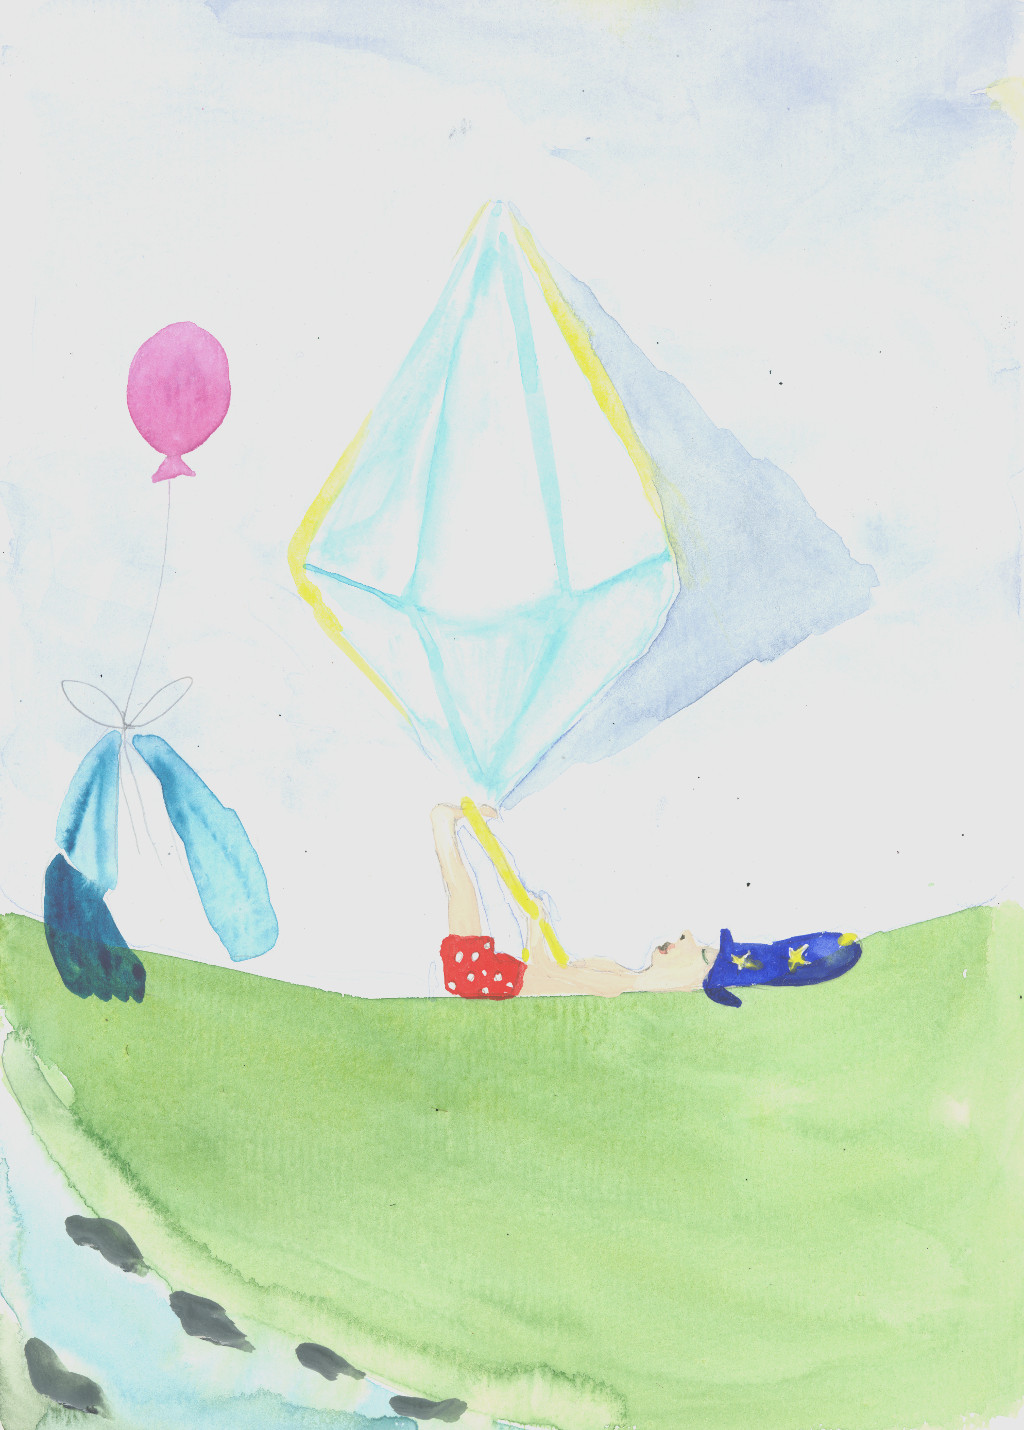
\includegraphics[width=12cm]{Anna2_smj}
					    %\vspace{2cm}
    				} 
                \end{minipage}
                \end{center}
               }
\end{adjustwidth}
%\part{Introduction to solid state physics}
%\end{adjustwidth}
\chapter{Lattice}
\lettrine[lines=3,slope=6pt,nindent=6pt]{\initfamily M}{o}st of us are familiar with "crystals" such as quartz and diamond with their typical crystal shapes: faces and vertices at specific angles. But metals as well as most solids are crystalline as well, just that their properties allow us to shape them macroscopically any way we want. It is their microscopic structure that determines their crystal properties. The microscopic structure can be determined by X-ray crystallography following the work of Bragg in 1913.\nl
It is sometimes possible to see the crystal structure directly in the naked eye. In Fig. \ref{fig:pyrite} we can see a rock containing three crystals of pyrite ($FeS_2$). The crystal structure of pyrite is cubic, which is reflected in the cubic symmetry of its natural crystal facets.
\begin{figure}[!ht] 
  \centering
  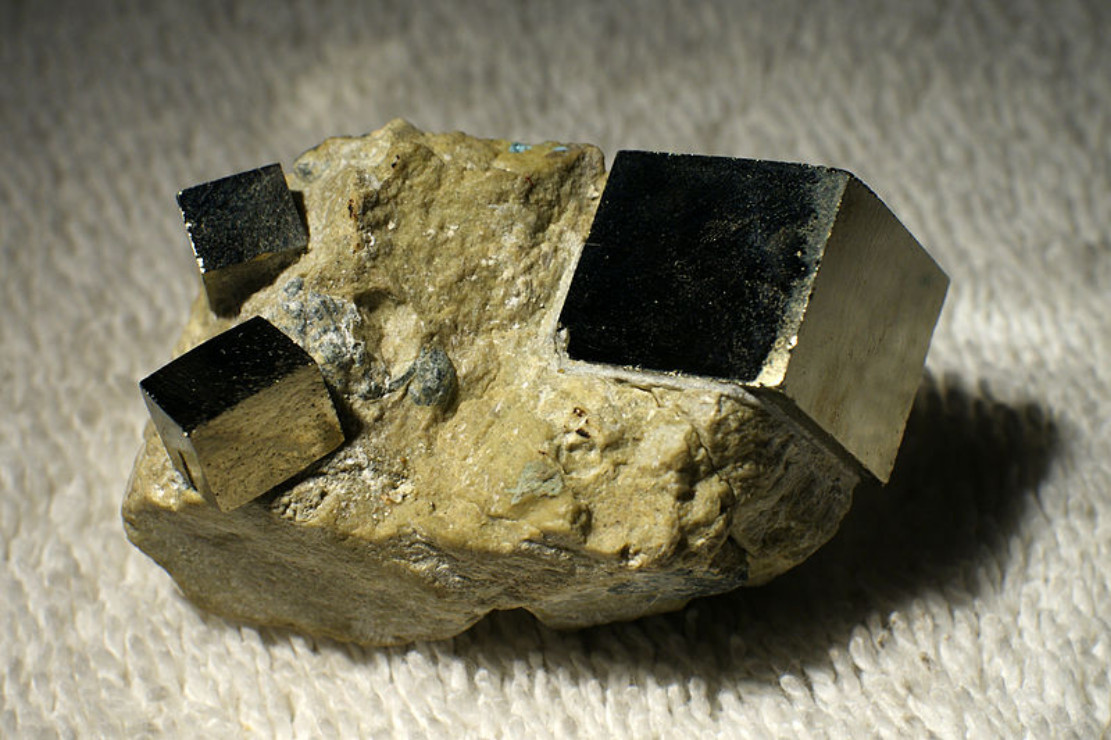
\includegraphics[width=14cm]{pyrite_cubesj.jpg}\\
  \caption{A rock containing three crystals of pyrite ($FeS_2$). The crystal structure of pyrite is cubic, which is reflected in the cubic symmetry of its natural crystal facets. \href{http://en.wikipedia.org/wiki/Pyrite}{(Wikipedia)}}
  \label{fig:pyrite}
\end{figure}
\section{Bravais lattice}
The \emph{Bravais lattice} specifies the periodic array in which the repeated units of the crystal are arranged. The units may be single atoms, groups of atoms, molecules, etc. The Bravais lattice summarizes the geometry of the underlying periodic structure. Here are two equivalent definitions of the Bravais lattice:
\begin{itemize}
\item A Bravais lattice is an infinite array of discrete points with an arrangement and orientation that appears exactly the same, from whichever of the points the array is viewed.
\item A (three dimensional) Bravais lattice consists of all points with position vectors $\vec{R}$ of the form,
\be 
\vec{R} = n_1 \vec{a}_1 + n_2 \vec{a}_2 + n_3 \vec{a}_3 \outnote{Lattice points}
\ee
where $\vec{a}_1,\vec{a}_2,\vec{a}_3$ are any three vectors not all in the same plane, and $n_1,n_2,n_3$ range through all integer values. 
\end{itemize}
The vectors $\vec{a}_i$ are called \emph{primitive vectors} and are said to \emph{generate} or \emph{span} the lattice.\nl
Fig. \ref{fig:bravais_2d} shows typical Bravais lattices in two dimensions, with the vectors $\vec{a}_1,\vec{a}_2$ outlined. Notice that both definitions for the Bravais lattice apply.
\begin{figure}[!ht]
  \centering
  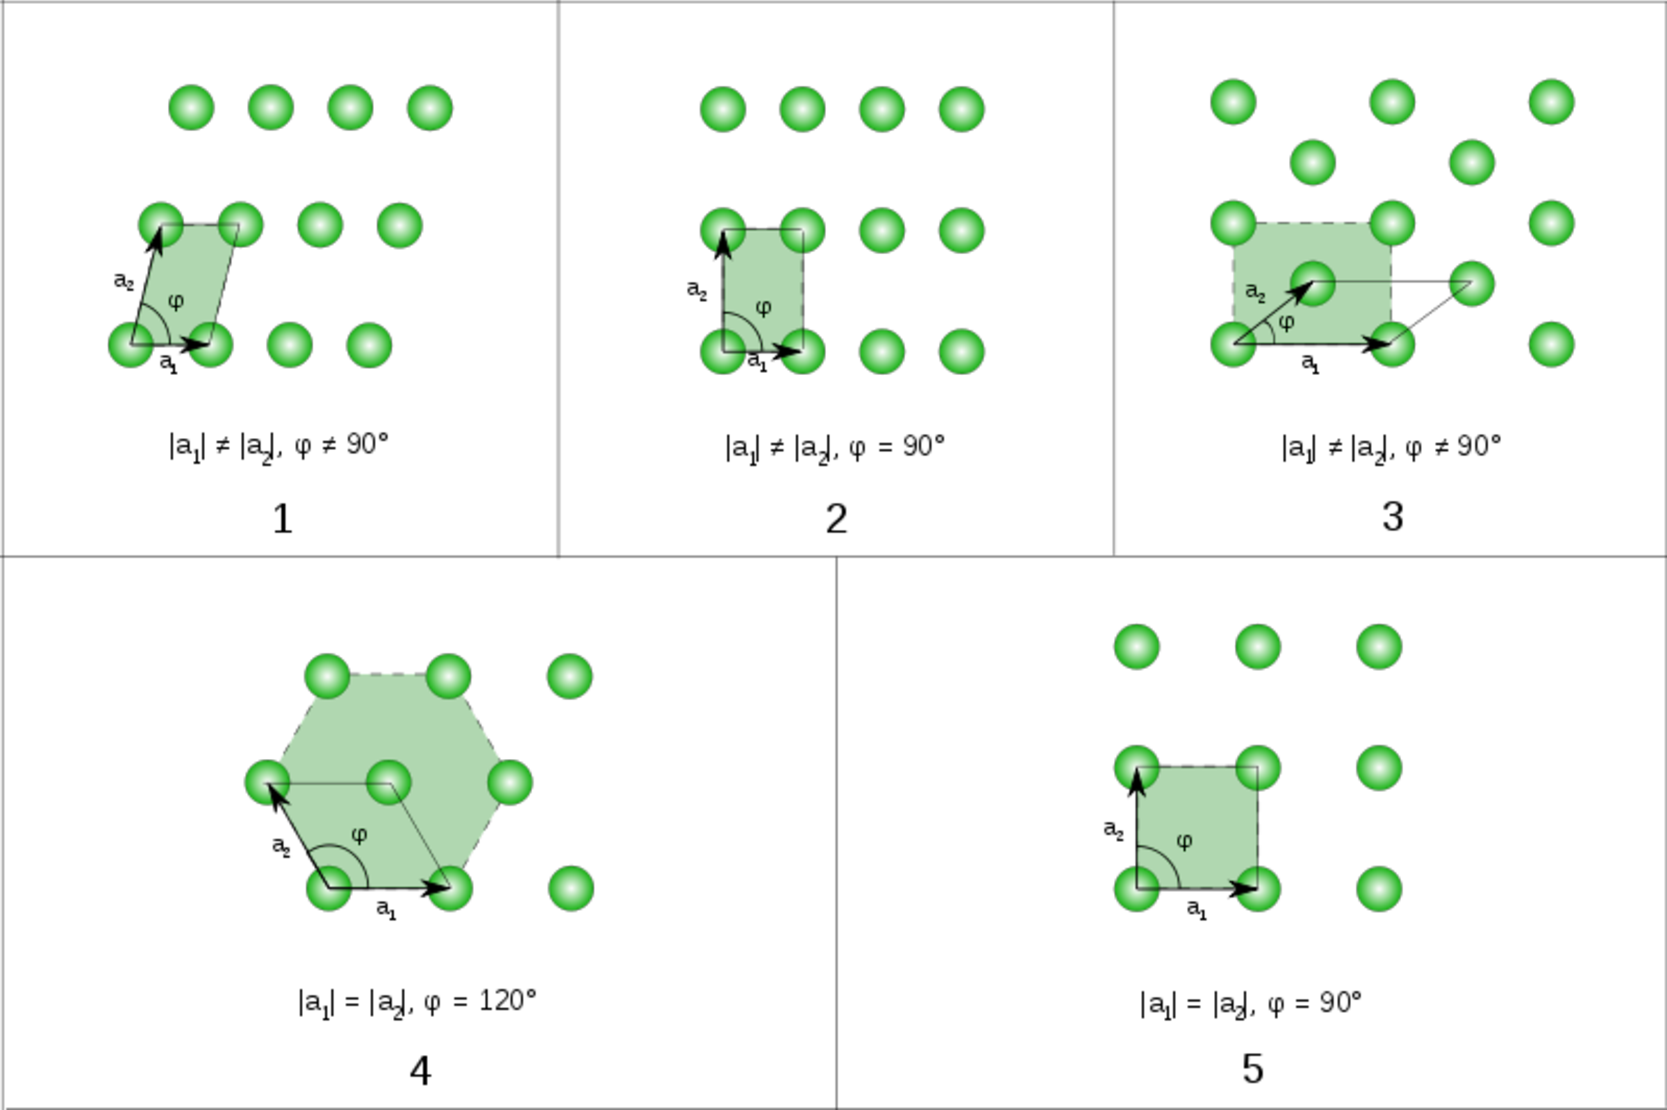
\includegraphics[width=14cm]{bravais_2d.pdf}\\
  \caption{The five fundamental two-dimensional Bravais lattices: 1 oblique, 2 rectangular, 3 centered rectangular (rhombic), 4 hexagonal, and 5 square. \href{http://en.wikipedia.org/wiki/Bravais_lattice}{(Wikipedia)}.}
  \label{fig:bravais_2d}
\end{figure}
Since all points on the lattice are equivalent, the Bravais lattice must be infinite in extent. Actual crystals are finite, but they are large enough that the majority of points will be so far from the surface that they unaffected by it. So putting surface effects aside, we need to consider a finite lattice only so that we can talk about the volume $V=L^3$. Then it is also natural to use periodic boundary conditions which mimic the infinite symmetry of an ideal lattice.
\section{Primitive vectors, BCC, FCC}
For a given Bravais lattice, the set of primitive vectors is not unique. This is true for both two and three dimensions. Consider the Body Centered Cubic (BCC) lattice shown in Fig. \ref{fig:bcc}. One can think of it as a simple lattice formed from points A with points B and the cube centers, or a simple cubic lattice formed from points B with points A at the cube centers.\nl 
%\begin{figure}
%  \centering
%  \subfigure[]{\includegraphics[width=0.49\hsize]{bcc1.pdf}}
%  \subfigure[]{\includegraphics[width=0.49\hsize]{bcc2.pdf}}
%  \caption{\textbf{(a)} BCC lattice as two displaced square lattices $A$ (black) and $B$ (red). \textbf{(b)} Suggestion for its primitive vectors from Eq. \ref{eq:bcc_primitive1}}
%  \label{fig:bcc}
%\end{figure}
\marginfig[-2.5in]{bcc_both_side.png}{BCC\label{fig:bcc}}
To describe the BCC lattice we can choose the primitive vectors to be,
\bea
\label{eq:bcc_primitive1}
\vec{a}_1 &=& a\vec{e}_x \nn
\vec{a}_2 &=& a\vec{e}_y \nn
\vec{a}_3 &=& \frac{a}{2}\left( \vec{e}_x + \vec{e}_y + \vec{e}_z\right)
\eea
A more symmetric choice is,
\bea
\label{eq:bcc_primitive2}
\vec{a}_1 &=& \frac{a}{2}\left( \vec{e}_y + \vec{e}_z - \vec{e}_x\right)\nn
\vec{a}_2 &=& \frac{a}{2}\left( \vec{e}_z + \vec{e}_x - \vec{e}_y\right)\nn
\vec{a}_3 &=& \frac{a}{2}\left( \vec{e}_x + \vec{e}_y - \vec{e}_z\right)
\eea
Another important example is the face-centered cubic (FCC) lattice. There, we take a simple cubic lattice and put another point at the center of every face. Fig. \ref{fig:FCC} shows the FCC.\nl
\begin{figure}
  \centering
  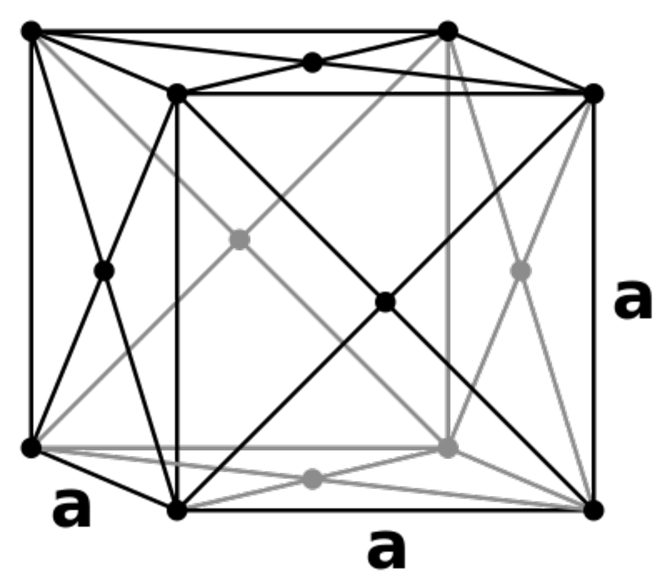
\includegraphics[width=8cm]{fcc2.pdf}\\
  \caption{An example of a face-centered-cubic (FCC) lattice. Lattice sites are marked as black dots; sides are all length $a$. \href{http://en.wikipedia.org/wiki/Cubic_crystal_system}{(Wikipedia)}}
  \label{fig:FCC}
\end{figure}
A symmetric set of primitive vectors for the FCC lattice is,
\bea
\vec{a}_1 &=& \frac{a}{2}\left( \vec{e}_y + \vec{e}_z\right)\nn
\vec{a}_2 &=& \frac{a}{2}\left( \vec{e}_z + \vec{e}_x \right)\nn
\vec{a}_3 &=& \frac{a}{2}\left( \vec{e}_x + \vec{e}_y \right) 
\eea
Here are (partial) lists of some elements with FCC and BCC structure:

\textbf{FCC}: Ar,Ag,Al,Au,Ca,Cu,La,Pb,Sr,Th 

\textbf{BCC}: Ba,Fe,K,Li,Na,Nb,Rb

\section{Wigner-Seitz Primitive Cell}
\personfeature[-4.4in]{Wigner}{Eugene Paul Wigner}{1902-1995}{was a Hungarian American theoretical physicist and mathematician. He received a share of the Nobel Prize in Physics in 1963 "for his contributions to the theory of the atomic nucleus and the elementary particles, particularly through the discovery and application of fundamental symmetry principles"; the other half of the award was shared between Maria Goeppert-Mayer and J. Hans D. Jensen. Wigner is notable for having laid the foundation for the theory of symmetries in quantum mechanics as well as for his research into the structure of the atomic nucleus. He first identified Xe-135 "poisoning" in nuclear reactors, and for this reason it is sometimes referred to as Wigner poisoning. Wigner is also important for his work in pure mathematics, having authored a number of theorems. In particular, Wigner's theorem is a cornerstone in the mathematical formulation of quantum mechanics. \href{http://en.wikipedia.org/wiki/Wigner}{(Wikipedia)}}
A primitive cell is a volume of space that, when translated through all the vectors in the Bravais lattice, just fills all of the space without either overlapping itself or leaving voids. There is no unique way of choosing a primitive cell for a given Bravais lattice. One way that keeps the symmetry of the lattice is the Wigner-Seitz cell.\nl
The Wigner-Seitz cell about a lattice point is the region of space that is closer to that point than to any other lattice point. Since there is nothing in the definition of the Wigner-Seitz cell that refers to any particular choice of primitive vectors, the Wigner-Seitz cell will be as symmetrical as the Bravais lattice. Fig. \ref{fig:wigner_seitz_2d} shows the construction in two dimensions. It is done by drawing lines connecting the point to all others in the lattice, bisecting each line with a plane and taking the smallest polyhedron containing the point bounded by these planes. 
\begin{figure}[!ht] 
  \centering
  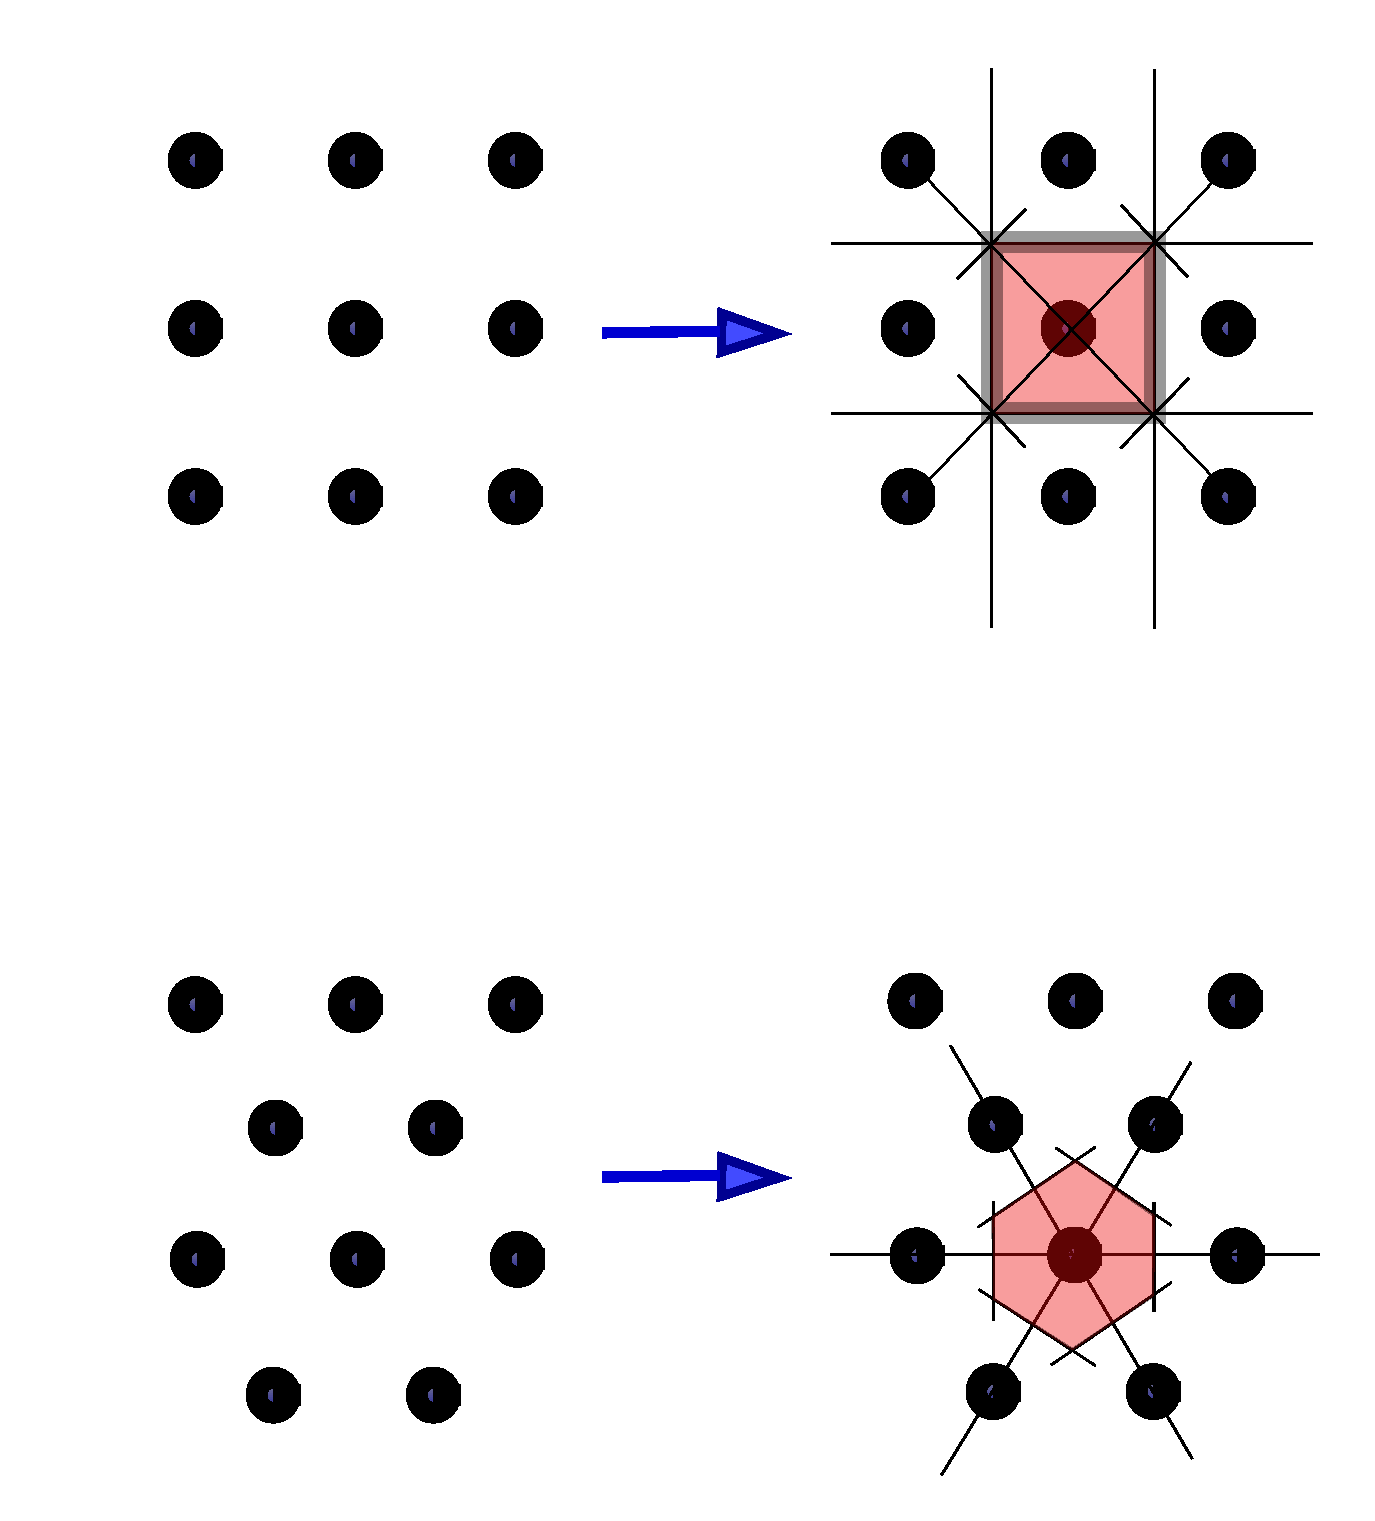
\includegraphics[width=10cm]{ws_2d2.pdf}\\
  \caption{Construction of a Wigner-Seitz primitive cell. The sides of the cell bisect the lines joining the central points to its nearest neighboring points. \href{http://en.wikipedia.org/wiki/Wigner\%E2\%80\%93Seitz_cell}{(Wikipedia)}}
  \label{fig:wigner_seitz_2d}
\end{figure}


%\begin{figure}
%  \centering
%  \subfigure[Brillouin zone for the BCC lattice.]{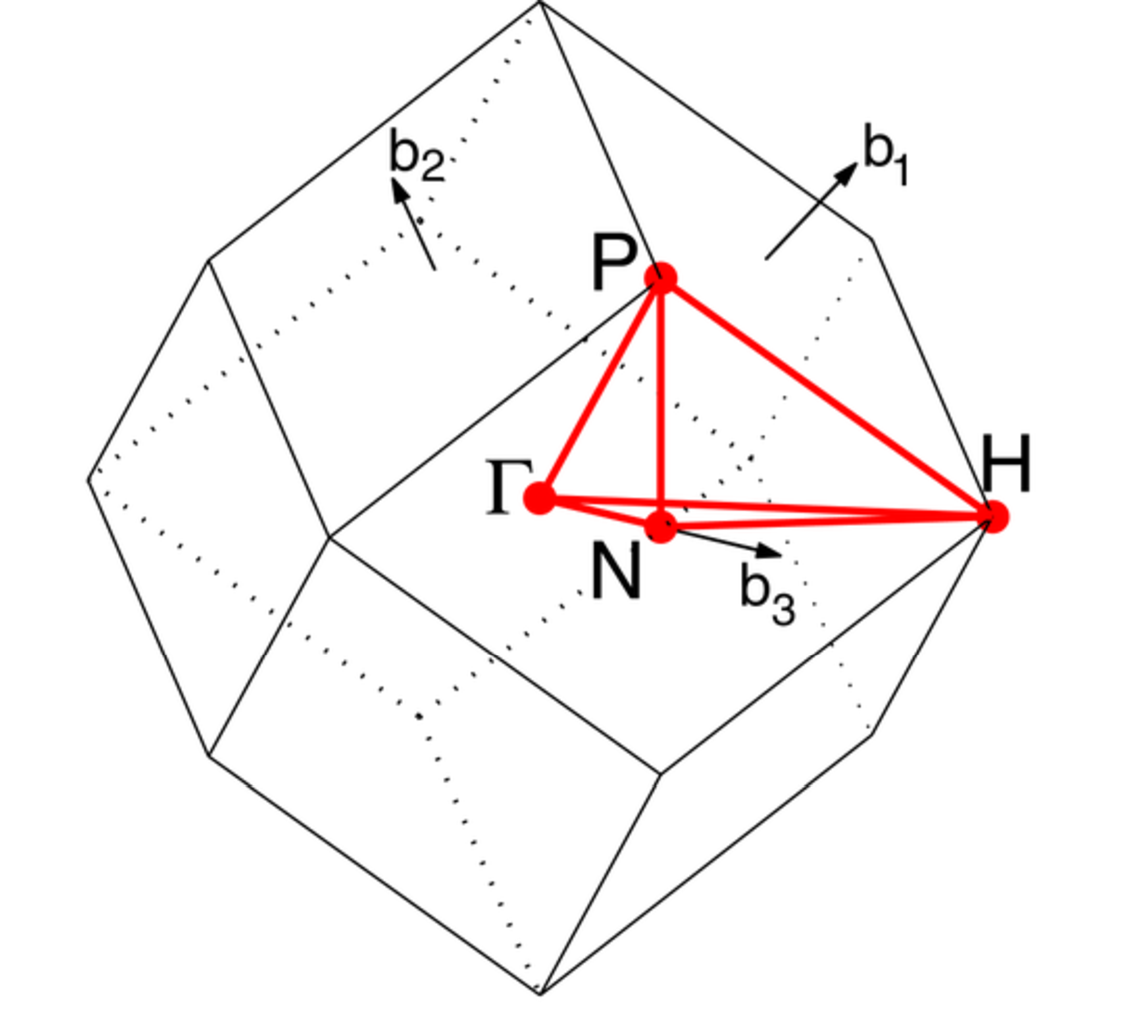
\includegraphics[width=0.49\hsize]{bcc_bz.pdf}}\\
%  \subfigure[Brillouin zone for the FCC lattice.]{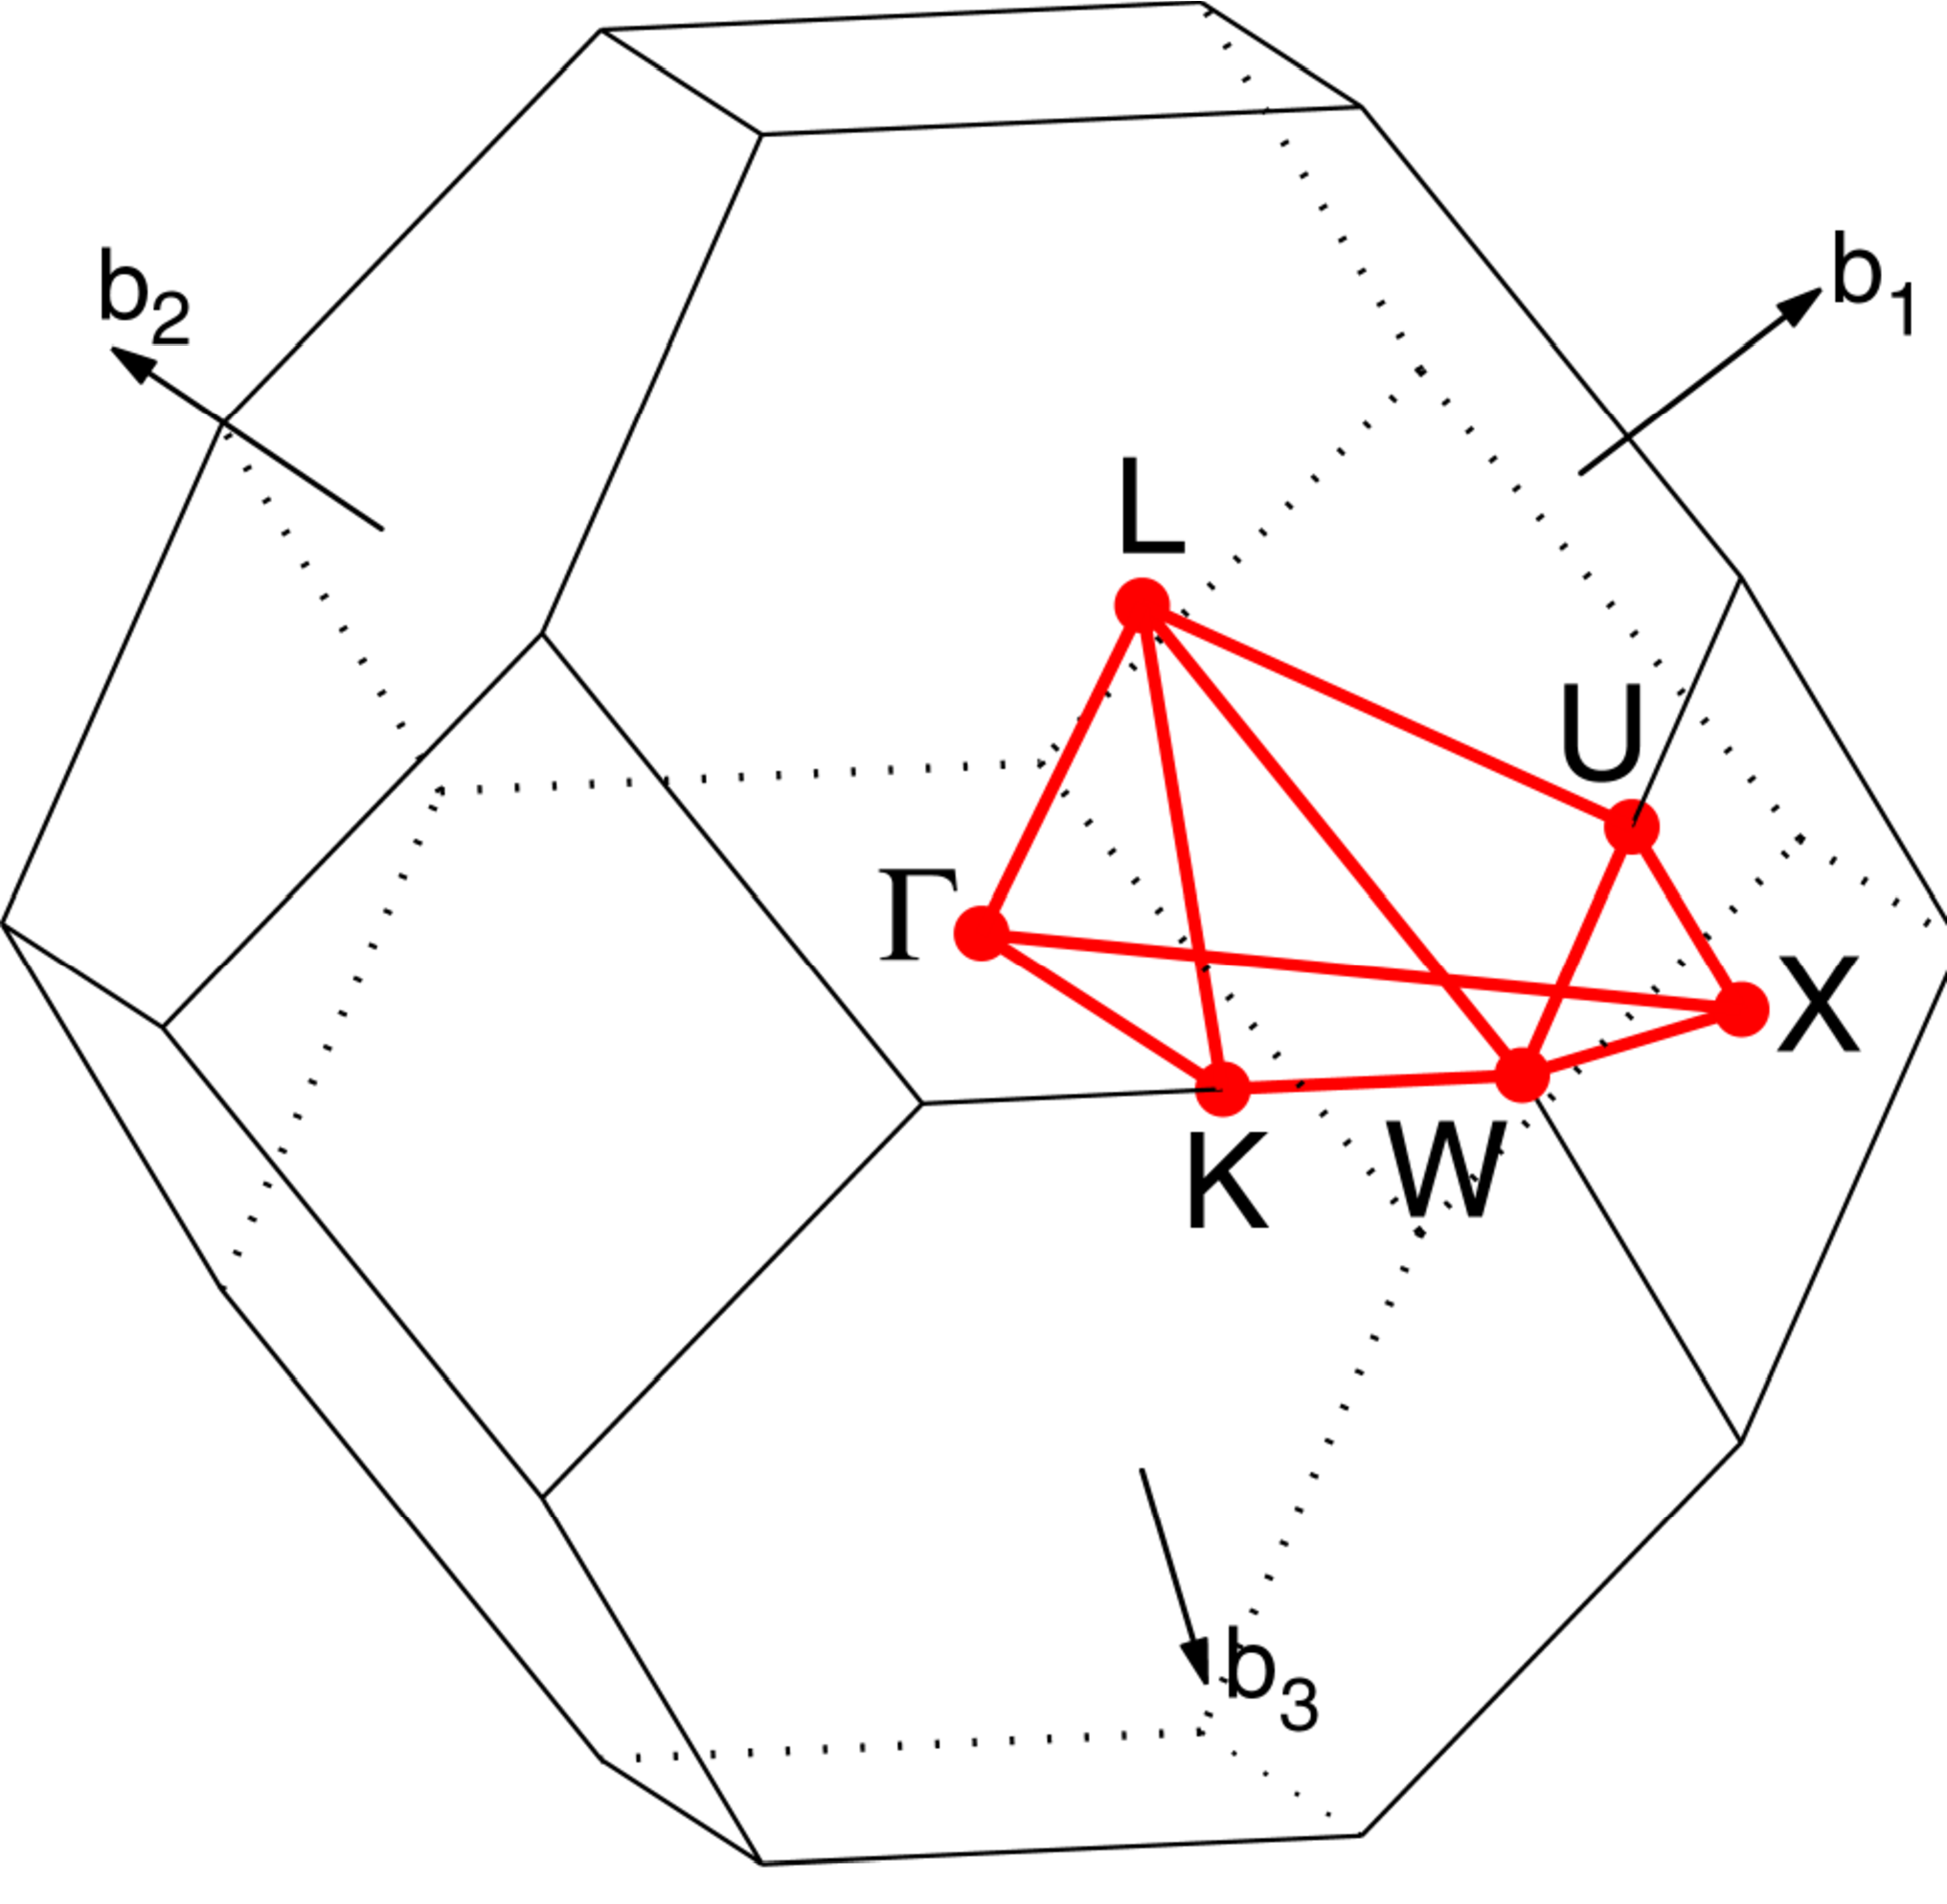
\includegraphics[width=0.49\hsize]{fcc_bz.pdf}}\\
%  \caption{Brillouin zones for the BCC and FCC lattices. From: Wikipedia (Auro69)}
%  \label{fig:wigner_seitz_bcc_fcc}
%\end{figure}

\section{The reciprocal lattice.}
The reciprocal lattice is a fundamental concept in solids. We will use it to study the periodic wave-functions. It can also be used to understand crystal diffraction, and to understand momentum conservation in a periodic structure, amongst other things. \nl
Consider a set of points $\vec{R}$ constituting a Bravais lattice and a plane wave $e^{i\vec{K}\vec{r}}$. For general $\vec{K}$, such a plane wave will not have the periodicity of the lattice, but certain special choices of the wave vector will.\nl
\emph{The set of all wave vectors $\vec{K}$ that have the periodicity of the lattice is known as its reciprocal lattice}. This means that $\vec{K}$ belongs to the reciprocal lattice of the Bravais lattice $\vec{R}$ if, for any $\vec{r}$ and all $\vec{R}$ in the lattice,
\be
e^{i\vec{K}(\vec{r}+\vec{R})} = e^{i\vec{K}\vec{r}}
\ee
This means that, for all $\vec{R}$ in the direct lattice, and all $\vec{K}$ in the reciprocal lattice,
\be 
e^{i\vec{K}\vec{R}} = 1 \outnote{Reciprocal lattice points}
\ee
The reciprocal lattice is also a Bravais lattice.\nl
Let $\vec{a}_1,\vec{a}_2,\vec{a}_3$ be a set of primitive vectors for the direct lattice. Then the reciprocal lattice primitive vectors can be generated as follows:
\bea 
\vec{b}_1 &=& 2\pi\, \frac{\vec{a}_2 \times \vec{a}_3}{\vec{a}_1\cdot (\vec{a}_2 \times \vec{a}_3)} \nn
\vec{b}_2 &=& 2\pi\, \frac{\vec{a}_3 \times \vec{a}_1}{\vec{a}_1\cdot (\vec{a}_2 \times \vec{a}_3)} \nn
\vec{b}_3 &=& 2\pi\, \frac{\vec{a}_1 \times \vec{a}_2}{\vec{a}_1\cdot (\vec{a}_2 \times \vec{a}_3)} 
\eea
We can see that,
\be
\vec{b}_i \cdot \vec{a}_j = 2\pi \delta_{ij}
\ee
and so for,
\bea
\vec{K} &=& k_1 \vec{b}_1 + k_2 \vec{b}_2 + k_3 \vec{b}_3 \nn
\vec{R} &=& n_1 \vec{a}_1 + n_2 \vec{a}_2 + n_3 \vec{a}_3 \nn
n_i,\, k_j &= & 0,\pm 1,\pm 2, ...
\eea
It follows that,
\be
\vec{K}\cdot \vec{R} = 2\pi(k_1 n_1 + k_2 n_2 + k_3 n_3) \quad \rightarrow \quad e^{i\vec{K}\cdot \vec{R}} = 1
\ee
We note that the reciprocal of the reciprocal lattice is the direct lattice.

\subsection{Examples:}
The simple cubic lattice has a cubic primitive cell of side $a$, has a simple cubic reciprocal lattice of side $2\pi/a$. ie.
\bea 
\vec{a}_1 = a\vec{e}_x, \quad \vec{a}_2 &=& a\vec{e}_y, \quad \vec{a}_3 = a\vec{e}_z \nn
\vec{b}_1 = \frac{2\pi}{a}\vec{e}_x, \quad \vec{b}_2 &=& \frac{2\pi}{a}\vec{e}_y, \quad \vec{b}_3 = \frac{2\pi}{a}\vec{e}_z \nn
\eea
The FCC lattice with side $a$ has as its reciprocal a BCC lattice with side $4\pi/a$. ie.
\bea 
\vec{a}_1 = \frac{a}{2}\left( \vec{e}_y + \vec{e}_z\right)\quad
\vec{a}_2 &=& \frac{a}{2}\left( \vec{e}_z + \vec{e}_x \right)\quad
\vec{a}_3 = \frac{a}{2}\left( \vec{e}_x + \vec{e}_y \right) \nn
\vec{b}_1 = \frac{2\pi}{a}\left( \vec{e}_y + \vec{e}_z - \vec{e}_x\right)\quad
\vec{b}_2 &=& \frac{2\pi}{a}\left( \vec{e}_z + \vec{e}_x - \vec{e}_y\right)\quad
\vec{b}_3 = \frac{2\pi}{a}\left( \vec{e}_x + \vec{e}_y - \vec{e}_z\right) 
\eea
Similarly, the reciprocal of the BCC lattice is the FCC lattice.\nl


\noindent The \textbf{first Brillouin zone} is the Wigner-Seitz primitive cell of the reciprocal lattice. Therefore, the first Brillouin zone (in short, BZ) of the BCC lattice is the Wigner-Seitz cell of the FCC lattice. Fig. \ref{fig:bcc_fcc_bz} shows the BZ for the BCC and FCC lattices.

\marginfig[-4.5in]{bcc_fcc_bz.png}{Brillouin zone for BCC and FCC lattices \href{http://en.wikipedia.org/wiki/Brillouin_zone}{(Wikipedia)} \label{fig:bcc_fcc_bz}}

%\begin{figure}[!ht] 
%  \centering
%  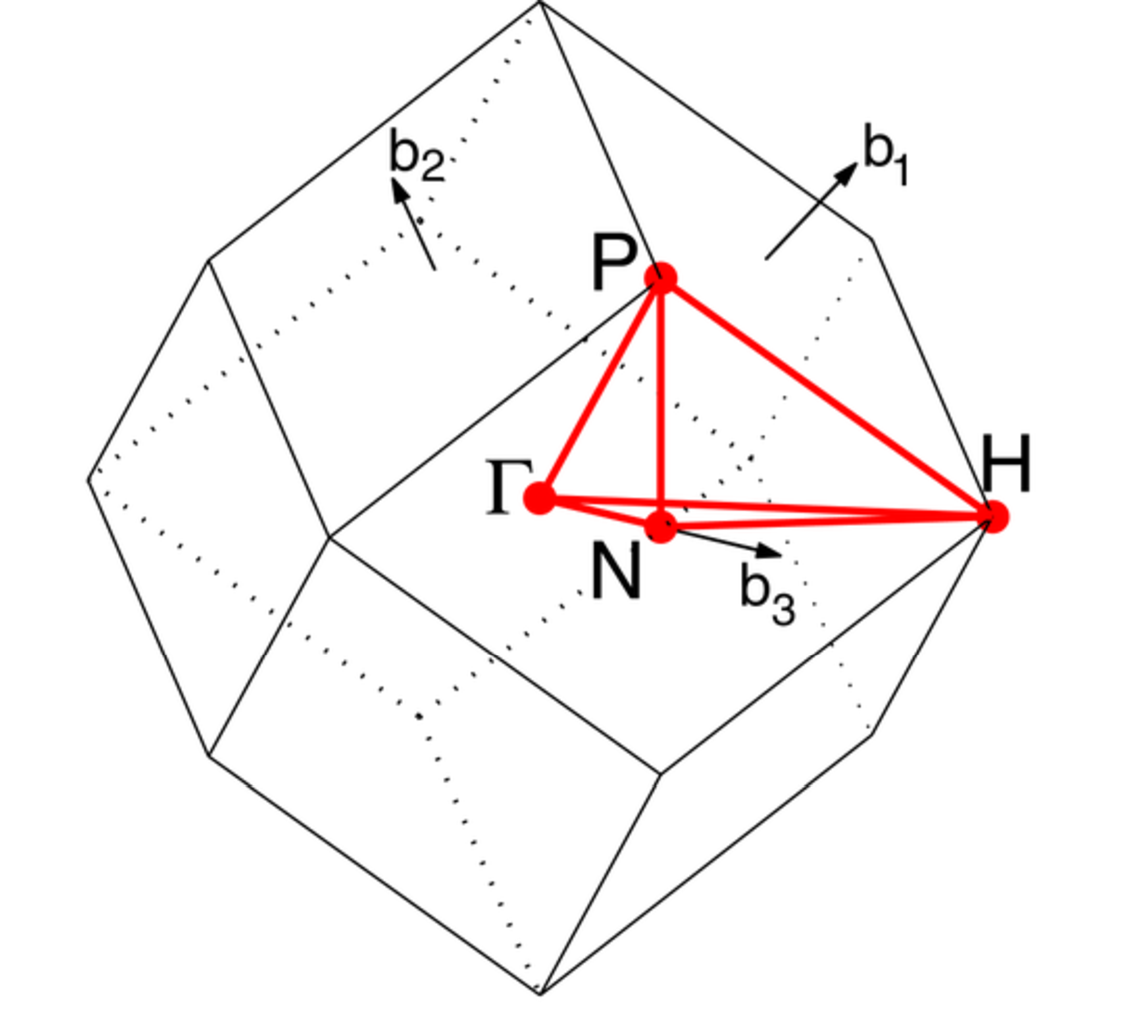
\includegraphics[width=5cm]{bcc_bz.pdf}\\
%  \caption{Brillouin zone for the BCC lattice. \href{http://en.wikipedia.org/wiki/Brillouin_zone}{(Wikipedia)}}
%  \label{fig:bcc_bz}
%\end{figure}
%
%\begin{figure}[!ht] 
%  \centering
%  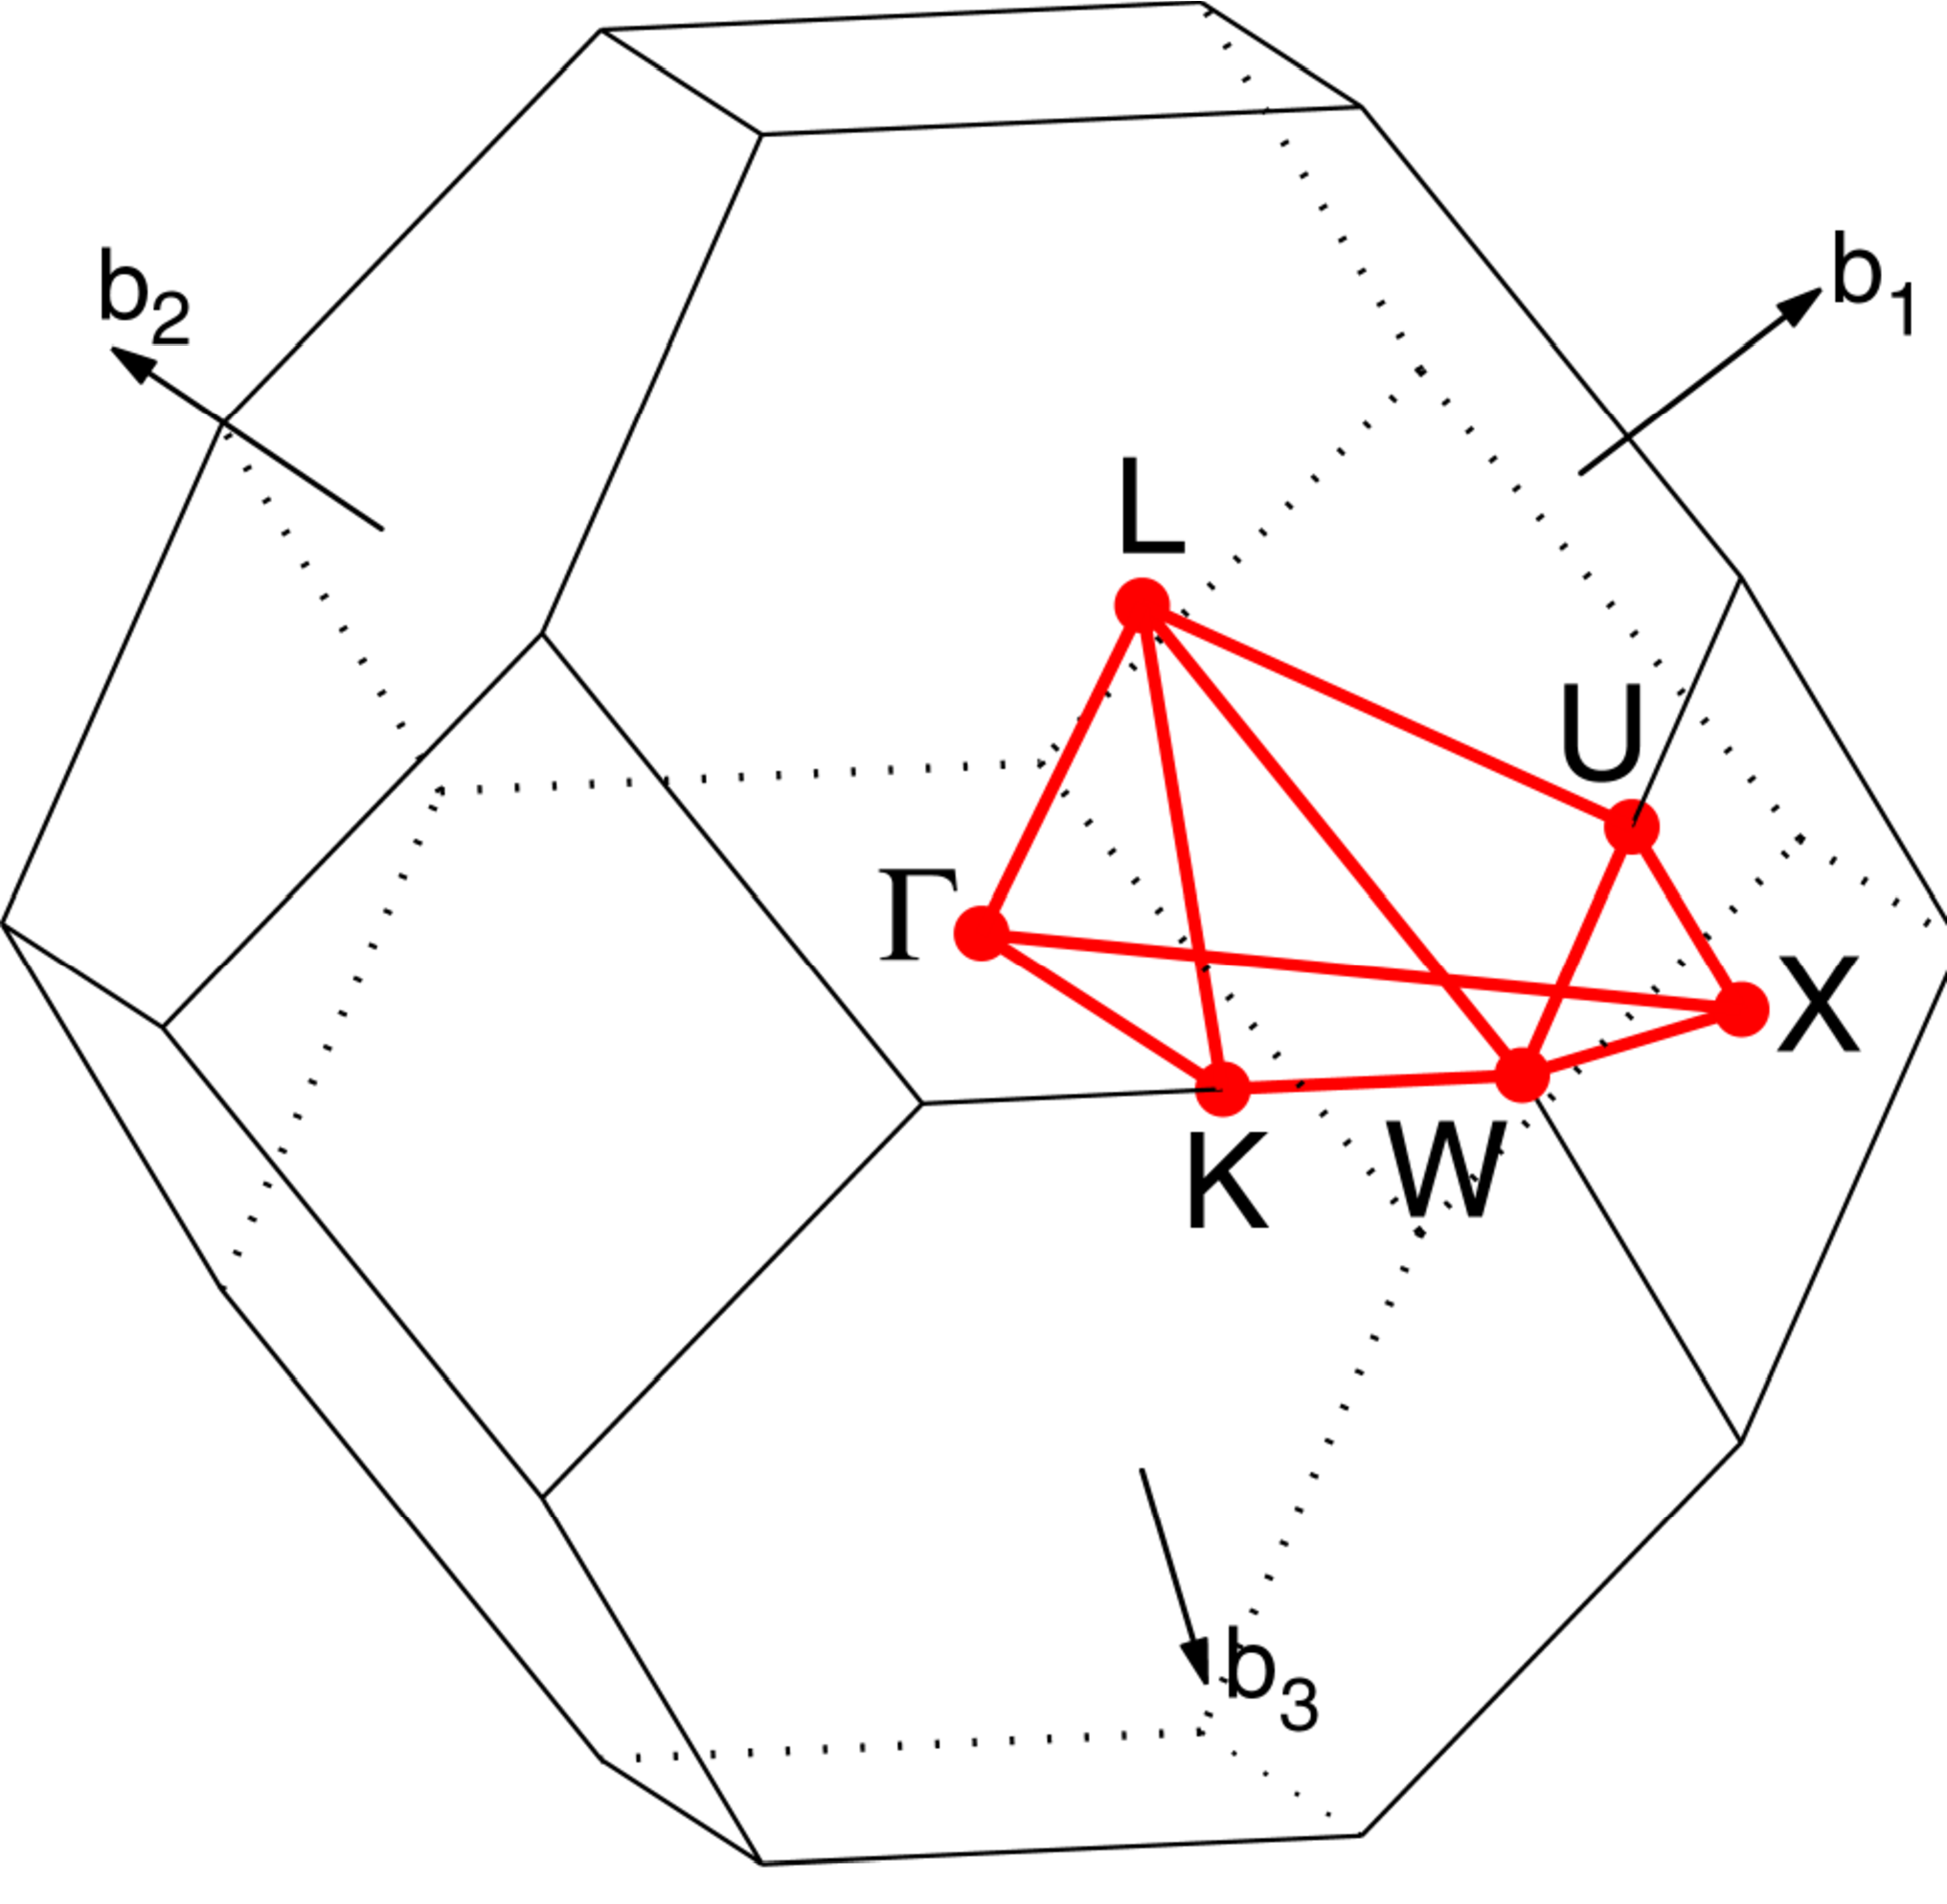
\includegraphics[width=5cm]{fcc_bz.pdf}\\
%  \caption{Brillouin zone for the FCC lattice. \href{http://en.wikipedia.org/wiki/Brillouin_zone}{(Wikipedia)}}
%  \label{fig:fcc_bz}
%\end{figure}

%%%%%%%%%%%%%%%%%%%%%%%%%%%%%%%%%%%%%%%%%%%%%%%%%%%%%%%%%%%%%%%%%%%%%%%%%%%%%%%%%%%%%%%%%

\chapter{Electrons in a periodic potential }
\lettrine[lines=3,slope=6pt,nindent=6pt]{\initfamily W}{e}'ve seen that solids have a crystal structure that is periodic. Let us think of the ions exerting a periodic electric potential with the periodicity of the Bravais lattice,
\be
U(\vec{r}+\vec{R}) = U(\vec{r}) \outnote{Periodic potential}
\ee
The scale of the periodicity of typical solids is $\approx 10^{-10}m$ which is approximately the de-Broglie wavelength for an electron at room temperature, so we need to use quantum mechanics for our calculations.\nl
In reality, solids are not ideal and have imperfections: dislocated ions or certain atoms replaced by a different element. In the theory of solids, we usually first understand the properties of an ideal lattice and then treat the change from the ideal as a small perturbation.\nl
In principle, the problem of electrons in a solid is a many-electron problem because of the Coulomb interaction between the electrons as well as the periodic interaction between the electrons and the ions in the lattice. The study of many-body physics or "correlated electrons" is an ongoing research effort which is needed to explain important physical behavior eg. superconductivity and magnetism. We limit ourselves to an \emph{independent electron} approximation in which each electron interacts only with an \emph{effective} one-electron potential $U(\vec{r})$ but otherwise \emph{we neglect electron-electron interactions}. The effective potential $U(\vec{r})$ contains some features of the electron-electron interaction but it is generally a very coarse approximation. Yet it simplifies the problem considerably, since now we need to solve for only one electron satisfying the Hamitonian,
\bea 
\hat{H} &=& \frac{\hat{p}^2}{2m} + U(\hat{\vec{r}}) \nn
U(\hat{\vec{r}}+\vec{R}) &=& U(\hat{\vec{r}})
\eea
\section{Bloch's theorem}
Bloch's theorem states the the solutions $\phi_{nk}(\vec{r})$ for the time-independent Schr{\"o}dinger equation (ie. the stationary states of the Hamiltonian) for a periodic potential $U(\vec{r})$ satisfy,
\be 
\phi_{nk}(\vec{r}+\vec{R}) = e^{i\vec{k}\cdot \vec{R}} \phi_{nk}(\vec{r}) \outnote{Bloch's Theorem I}
\ee
for every $\vec{R}$ in the Bravais lattice.\nl
Another way to state Bloch's theorem is,
\be 
\phi_{nk}(\vec{r}) = e^{i\vec{k}\cdot \vec{r}} u_{nk}(\vec{r}) \outnote{Bloch's Theorem II}
\ee
with $u$ periodic, ie. $u_{nk}(\vec{r}+\vec{R}) = u_{nk}(\vec{r})$.\nl
\textbf{Proof:} For every Bravais lattice vector $\vec{R}$ we define a translation operator $T_{\vec{R}}$ such that, when operating on any function $f(\vec{r})$,
\be
T_{\vec{R}} f(\vec{r}) = f(\vec{r}+\vec{R}) 
\ee
Since the Hamiltonian is periodic, we have,
\bea 
T_{\vec{R}} \hat{H} \phi &=& \hat{H}(\vec{r}+\vec{R})\phi(\vec{r}+\vec{R}) \nn
 &=& \hat{H}(\vec{r})\phi(\vec{r}+\vec{R}) = \hat{H} T_{\vec{R}} \phi
\eea
since this is true for any function $\phi$ then $T_{\vec{R}}$ and $\hat{H}$ commute, ie.
\personfeature[-0.5in]{Bloch}{Felix Bloch}{1905-1983}{was a Swiss physicist, winner of the 1952 Nobel Prize together with Edward Mills Purcell for "their development of new ways and methods for nuclear magnetic precision measurements." In 1933, immediately after Hitler came to power, he left his position in Leipzig, Germany because he was Jewish. During WW II he worked on nuclear power at Los Alamos National Laboratory, before resigning to join the radar project at Harvard University. After the war he concentrated on investigations into nuclear induction and nuclear magnetic resonance, which are the underlying principles of MRI. In 1946 he proposed the Bloch equations which determine the time evolution of nuclear magnetization. In 1954, he served for one year as the first Director-General of CERN. \href{http://en.wikipedia.org/wiki/Wigner}{(Wikipedia)}}
\be 
T_{\vec{R}} \hat{H} = \hat{H} T_{\vec{R}} 
\ee
We know than when two operators commute, the eigenbasis of one is also an eigenbasis of the other, meaning that the stationary states $\phi_{nk}(\vec{r})$ are eigenstates of both $\hat{H}$ and $T_{\vec{R}}$, ie.
\bea 
\hat{H} \phi_{nk}(\vec{r}) &=& E_{nk} \phi_{nk}(\vec{r})  \nn
T_{\vec{R}} \phi_{nk}(\vec{r}) &=& c(\vec{R}) \phi_{nk}(\vec{r})
\eea
Notice also that translations commute, so that,
\bea 
T_{\vec{R}}T_{\vec{R'}}\phi_{nk}(\vec{r}) &=& T_{\vec{R'}} T_{\vec{R}}\phi_{nk}(\vec{r}) = \phi_{nk}(\vec{r}+\vec{R}+\vec{R}')\nn
T_{\vec{R}}T_{\vec{R'}} &=& T_{\vec{R'}}T_{\vec{R}} = T_{\vec{R}+\vec{R'}}\nn
T_{\vec{R}}T_{\vec{R'}} \phi_{nk}(\vec{r}) &=& T_{\vec{R}} C(\vec{R}') \phi_{nk}(\vec{r})  = C(\vec{R}) C(\vec{R}') \phi_{nk}(\vec{r}) \nn
T_{\vec{R}+\vec{R'}} \phi_{nk}(\vec{r}) &=& C(\vec{R}+\vec{R}') \phi_{nk}(\vec{r}) \nn
  C(\vec{R}+\vec{R}') &=& C(\vec{R})C(\vec{R}')
\eea
Now let $\vec{a}_i$ be the primitive vectors for the Bravais lattice. Without limiting $x_i$, we can always write,
\be 
C(\vec{a}_i) = e^{2\pi i x_i}
\ee
So that for any $\vec{R}$ in the Bravais lattice,
\be 
\vec{R} = n_1 \vec{a}_1 + n_2 \vec{a}_2 + n_3 \vec{a}_3
\ee
we have,
\be 
C(\vec{R}) = c(\vec{a}_1)^{n_1}c(\vec{a}_2)^{n_2}c(\vec{a}_3)^{n_3}
\ee
so that,
\bea
C(\vec{R}) &=& e^{i\vec{k}\cdot \vec{R}} \nn
\vec{k} &=& x_1 \vec{b}_1 + x_2 \vec{b}_2 + x_3 \vec{b}_3
\eea
with the $\vec{b}_i$ the reciprocal lattice vectors, meaning that they obey the relation,
\be 
\vec{b}_i\cdot\vec{a}_j = 2\pi \delta_{ij}
\ee
Summarizing, we see that for every Bravais lattice vector $\vec{R}$ we can choose the eigenvalues of $\hat{H}$, $\phi_{nk}(\vec{r})$ such that,
\be 
T_{\vec{R}} \phi_{nk}(\vec{r}) = \phi_{nk}(\vec{r}+\vec{R}) = C(\vec{R})\phi_{nk}(\vec{r}) = e^{i\vec{k}\cdot \vec{R}} \phi_{nk}(\vec{r})
\ee
This is Bloch's theorem.\nl
We have discussed already the usefulness of setting periodic boundary conditions to the whole lattice, keeping things symmetric. So we set the total length in the $i$ direction to be $N_i$ times the primitive vector $a_i$. Now the periodic boundary conditions on the lattice give,
\be 
\phi_{nk}(\vec{r}+N_i \vec{a}_i) = \phi_{nk}(\vec{r})
\ee
which means that,
\bea 
e^{iN_i \vec{k}\cdot \vec{a}_i} &=& 1, \quad \,\,\,\, i=1,2,3 \nn
e^{2\pi i N_i x_i} &=& 1 
\eea
so that $x_i$ must be real and a ratio of two integers,
\be
x_i = \frac{m_i}{N_i}, \quad \,\,\,\, m_i = 1,2,3,..., N_i 
\ee
so that the allowed Bloch wave vectors are quantized according to,
\be 
\vec{k} = \sum_{i=1}^3 \frac{m_i}{N_i} \vec{b}_i
\ee
and the volume of a an allowed value of $\vec{k}$ is 
\be
\frac{\vec{b_1}}{N_1}\cdot \left(\frac{\vec{b_2}}{N_2} \times \frac{\vec{b_3}}{N_3} \right) = \frac{1}{N} \vec{b_1}\cdot \vec{b}_2\times \vec{b}_3 
\ee
the product $\vec{b_1}\cdot \vec{b}_2\times \vec{b}_3$ is simply the volume of a primitive cell of the reciprocal lattice (Brilluin zone) so that \emph{the number of allowed wave vectors in the Brillouin zone is equal to the number of sites in the crystal}. Typically, in a macroscopic crystal, there are very many $\sim 10^{23}$ sites in the lattice, so that $k$ can be regarded as almost continuous. 
\subsection{Crystal Momentum}
Bloch's theorem introduces a wave vector $\vec{k}$ which behaves a lot like the free electron vector $\vec{k}$. Yet, for the free electron, $\vec{p} = \hbar \vec{k}$ where $\vec{p}$ is the momentum of the electron. In the Bloch case, $\hbar\vec{k}\ne\vec{p}$ ie. $\vec{k}$ is \emph{not} proportional to the momentum of the electron.  We can see this by $\vec{p} = -i\hbar \vec{\nabla}$ so that,
\be 
-i\hbar \vec{\nabla} \phi_{nk}(\vec{r}) = -i\hbar \vec{\nabla}\left(e^{i\vec{k}\cdot \vec{r}}u_{nk}(\vec{r}) \right) = \hbar \vec{k}\phi_{nk}(\vec{r})  -i\hbar e^{i\vec{k}\cdot \vec{r}} \vec{\nabla}u_{nk}(\vec{r})
\ee
So that $\phi_{nk}(\vec{r})$ is not a momentum eigenstate.\nl
We call $\hbar\vec{k}$ the \emph{crystal momentum} and we can think of it as a quantum number that characterizes the discrete translational symmetry of a periodic potential. $\vec{p}$ characterizes the continuous translational symmetry of the free space.
\subsection{First Brillouin Zone}
The wave vector $\vec{k}$ in Bloch's theorem can always be confined to the first Brillouin zone because any $\vec{k}'$ not in the first BZ, we can write,
\be 
\vec{k}' = \vec{k} + \vec{K}
\ee
with $\vec{K}$ a reciprocal lattice vector and $\vec{k}$ in the first BZ. Since $e^{i\vec{K}\cdot \vec{R}}=1$ for any reciprocal lattice vector, if Bloch's theorem holds for $\vec{k}'$ it also holds for $\vec{k}$. This means that we can restrict all our calculations to the first Brilluoin zone.
\subsection{The band index \texorpdfstring{$n$}{n}}
The index $n$ appears in Bloch's theorem because for a given $\vec{k}$ there are many solutions to the Schr{\"o}dinger equation. Let's look at all solutions for a specific $\vec{k}$ such that,
\be 
\phi_{nk}(\vec{r}) = e^{i\vec{k}\cdot \vec{r}} u_{nk}(\vec{r})
\ee
with $u$ having the periodicity of the lattice as before. Substituting into the Schodinger equation, $u$ is determined as the solutions for
\be 
\label{eq:H_bloch}
\hat{H}_k u_{nk}(\vec{r}) = \left( \frac{\hbar^2}{2m}\left(-i\vec{\nabla} + \vec{k} \right)^2 + U(\vec{r}) \right)u_{nk}(\vec{r}) = E_{nk} u_{nk}(\vec{r})
\ee
with the periodic boundary condition 
\be 
\label{eq:peru}
u_{nk}(\vec{r}) = u_{nk}(\vec{r}+\vec{R})
\ee
Because of the periodic boundary condition Eq. \ref{eq:peru}, we can treat Eq. ~\ref{eq:H_bloch} as an eigenvalue problem in a single primitive cell of the crystal. So we have an eigenvalue problem set in a finite space, which we have encountered before. We can expect an \emph{infinite} family of solutions labelled by $n$, with \emph{discretely} spaced energy eigenvalues $E_{nk}$. We call $n$ the band index. Note that in terms of Eq. \ref{eq:H_bloch}, $\vec{k}$ the Bloch wavevector is simply a parameter in the Hamiltonian. So we can expect the energies $E_n(\vec{k})$ to be continuous functions in $\vec{k}$. 
\subsection{Energy bands}
For a given band $n$, the eigenstates and eigenvalues are periodic functions of $\vec{k}$ in the reciprocal lattice, such that,
\bea 
\phi_{n,\vec{k}+\vec{K}}(\vec{r}) &=& \phi_{n,\vec{k}}(\vec{r}) \nn
E_{n,\vec{k}+\vec{K}} &=& E_{n,\vec{k}}
\eea
So we can describe the energy levels of an electron in a periodic potential in terms of a family of continuous functions $E_{n}(\vec{k})$ with the periodicity of the reciprocal lattice. The information contained in these function is referred to as the \emph{band structure} of the solid.\nl
For each $n$, the set of all electronic levels specified by $E_n(\vec{k})$ is called an \emph{energy band}. We note that since $E_n(\vec{k})$ are periodic in $\vec{k}$ and continuous, it has an upper and lower bound, so that all the levels $E_n(\vec{k})$ lie in between these two limits.
\subsection{Comparison between free and Bloch electrons}
We can now compare the two types of electrons we have learned about: the free electrons which we discussed in the infinite potential well and the Bloch electrons we have just discussed (electrons in a periodic potential):

\noindent \begin{tabular}{|l|l|l|}
\hline
 & Free electrons & Bloch \\
 \hline
Quantum numbers (no spin) & $\vec{k}$ is the momentum & $\hbar \vec{k}$ crystal momentum; $n$ band index\\ 
 \hline
Range of quantum numbers & $\vec{k}$ in all space, quantized & $n\in[1,\infty)$ integers; $\vec{k}$ all vectors in 1st BZ \\
\hline
Energy & $E(k)= \frac{\hbar^2k^2}{2m}$ & Unspecified. But $E_n(\vec{k}+\vec{K})=E_n(\vec{k})$ for $\vec{K}$ \\
& & in the reciprocal lattice. \\
\hline
Velocity & $\vec{v} = \frac{\hbar\vec{k}}{m} = \frac{1}{\hbar}\frac{\partial E(\vec{k})}{\partial k}$ & $\vec{v}_n(\vec{k})=\frac{1}{\hbar}\frac{\partial E_n(\vec{k})}{\partial k}$ \\
\hline
Wave function & $\phi_k(\vec{r}) = \frac{1}{\sqrt{V}}e^{i\vec{k}\cdot\vec{r}}$ & Unspecified. But $\phi_{nk}(\vec{r})=e^{i\vec{k}\cdot\vec{r}}u_{nk}(\vec{r})$ \\
&& with $u_{nk}(\vec{r}+\vec{R})=u_{nk}(\vec{r})$; $\vec{R}$ in lattice \\
\hline
\end{tabular}
\section{The Kronig-Penney model}
The Kronig-Penney model demonstrates that a simple one-dimensional periodic potential yields energy bands as well as energy band gaps. While it is an oversimplification of the three-dimensional potential and band structure in an actual crystal, it is an instructive tool to demonstrate how the band structure can be calculated for a periodic potential, and how allowed and forbidden energies are obtained when solving the Schr{\"o}dinger equation. 

\noindent The potential assumed in the model is shown in the Fig. \ref{fig:Kronig_Penney}.
%
\be 
U(x) = \left\{ \begin{array}{cc}
			0 & 0<x<a \\
			U_0 & -b < x< 0
\end{array}.\right.
\ee
\begin{figure}
  \centering
  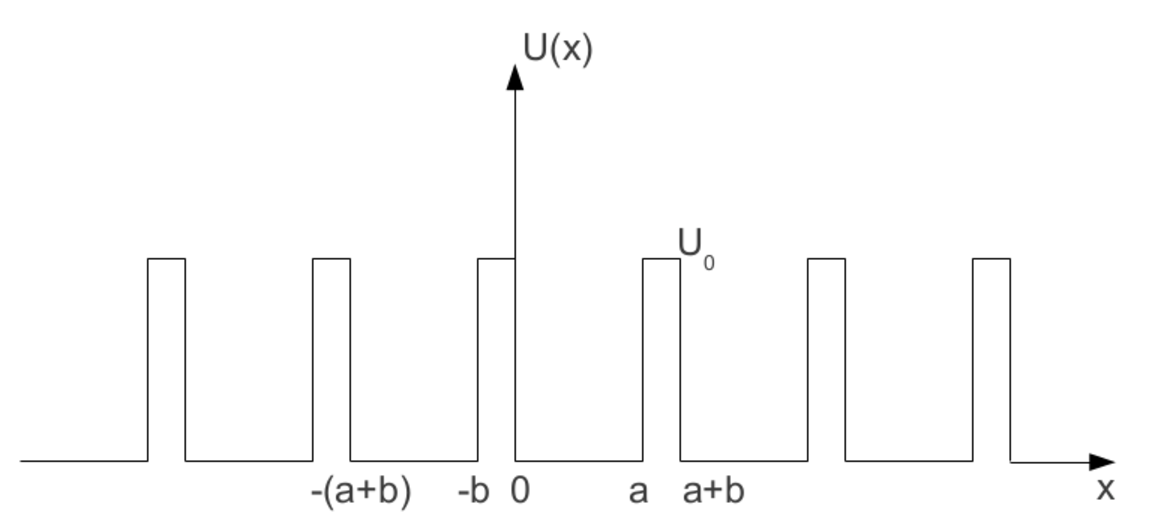
\includegraphics[width=15cm]{kronig_penney.pdf}
  \caption{The Periodic Kronig-Penney potential in one dimension. The lattice constant is $a$ and the potential is periodic in $a$.}
  \label{fig:Kronig_Penney}
\end{figure}
We need to solve the Schr{\"o}dinger equation,
\be
\left(-\frac{\hbar^2}{2m} \frac{d^2}{dx^2} + U(x) \right)\phi_{nk}(x) = E_{nk}\phi_{nk}(x)
\ee
Using Bloch's theorem, we only need to find a solution for a single period.\nl
Assuming that $E<U_0$, 
\bea 
\phi_{kn}(x) &=& \left\{ \begin{array}{cc}
			A e^{iKx} + B e^{-iKx} & 0 < x< a\\
			C e^{Qx} + De^{-Qx} & -b <x < 0
\end{array}.\right. \nn
K &=& \sqrt{\frac{2mE}{\hbar^2}} \nn
Q &=& \sqrt{\frac{2m(U_0-E)}{\hbar^2}}
\eea
Bloch's theorem means that,
\be 
\phi_{nk}(a<x<a+b) = \phi_{nk}(-b<x<0)e^{ik(a+b)}
\ee
which defines the Bloch wavevector $k$ used as an index to label the solution. The constants $A,B,C,D$ are chosen so that $\phi,\phi'$ are continuous at $x=0$ and $x=a$. At $x=0$,
\bea 
A+B &=& C+D \nn
iK(A-B) &=& Q(C-D)
\eea
At $x=a$ using the Bloch condition, meaning that $\phi(-b)e^{ik(a+b)} = \phi(a)$ and $\phi'(-b)e^{ik(a+b)}=\phi'(a)$ we have,
\bea
Ae^{iKa} + Be^{-iKa} &=& \left( Ce^{-Qb} + De^{Qb} \right)e^{ik(a+b)} \nn
iK\left(Ae^{iKa} - Be^{-iKa}\right) &=& Q\left( Ce^{-Qb} - De^{Qb} \right)e^{ik(a+b)}
\eea
The above four equations have a solution only if the determinant of the coefficients vanishes, 
\be 
\left\vert \begin{array}{cccc}
1 & 1 & -1 & -1 \\
iK & -iK & -Q & Q \\
e^{iKa} & e^{-iKa} & -e^{-Qb}e^{ik(a+b)} & -e^{Qb}e^{ik(a+b)} \\
iKe^{iKa} & -iK e^{-iKa} & -Qe^{-Qb}e^{ik(a+b)} & Q e^{Qb}e^{ik(a+b)}
\end{array} \right\vert= 0
\ee
meaning that (skipping some algebra...),
\be 
\left(\frac{Q^2-K^2}{2QK}\right)\sinh{Qb}\sin{Ka} + \cosh{Qb}\cos{Ka} = \cos{k(a+b)}
\ee
We can simplify the result be taking the limit $b\rightarrow 0$ and $U_0\rightarrow \infty$ while keeping $Q^2ba/2=P=const$. In this limit, $Q\gg K$ and $Qb \ll 1$. So we have,
\be 
f(Ka) = \frac{P}{Ka}\sin{Ka} + \cos{Ka} = \cos{ka}
\ee
We notice that the only allowed energies are those for which $-1 \le f(Ka)\le 1$. Fig. \ref{fig:KP_allowed_energies} shows this graphically for a choice $P=3\pi/2$. Whenever $f(Ka)$ is outside the domain $[-1,1]$, there are no solutions.\nl
\begin{figure}[!ht] 
  \centering
  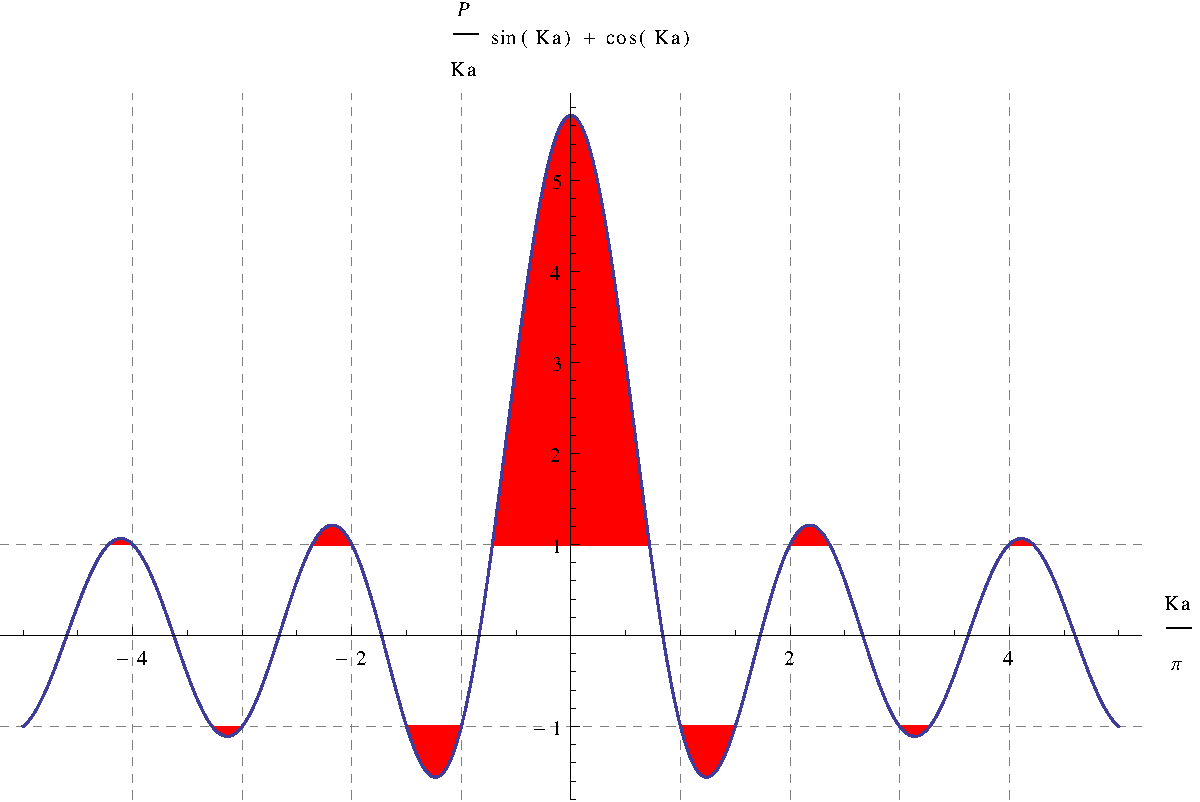
\includegraphics[width=15cm]{KP_allowed_energies.pdf}
  \caption{$f(Ka)$ for $P=3\pi/2$. The allowed values of the energy $E$ are given by those ranges of $Ka=a\sqrt{\frac{2mE}{\hbar^2}}$ for which the function lies between $\pm 1$. For other values of the energy (shaded red) there are no solutions to the Schr{\"o}dinger equation under the Bloch condition.}
  \label{fig:KP_allowed_energies}
\end{figure}
The important index is the Bloch wavevector $k$ and not $K$. Solving for $k$ we see the dependence of the energy and the formation of bands in Fig. \ref{fig:energy_bands}. The plot extends outside the first BZ to show the different $n$ solutions. The dashed line is the parabola $\frac{2mE}{\hbar^2}=k^2$ corresponding to free electrons. Notice that a gap opens in the energy spectrum at $k = \frac{\pi}{a}n$.
\begin{figure}[!ht] 
  \centering
  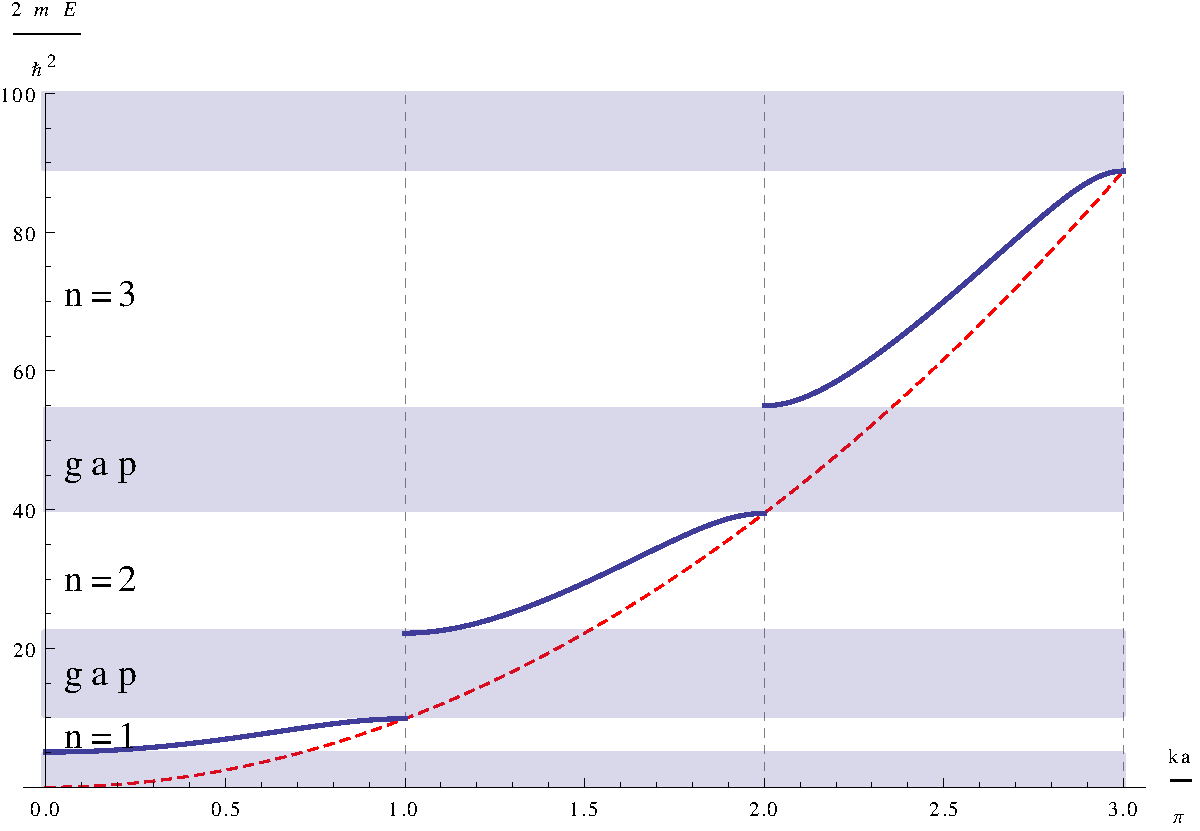
\includegraphics[width=15cm]{zones_ext.pdf}
  \caption{$E_n(k)$ vs. $k$. shown in the extended zone scheme. The plot extends outside the first BZ to show the different $n$ solutions. The dashed (red) line is the parabola $\frac{2mE}{\hbar^2}=k^2$ corresponding to free electrons. Notice that gaps open in the energy spectrum at integer $\frac{ka}{\pi}$.}
  \label{fig:energy_bands}
\end{figure}
%%%%%%%%%%%%%%%%%%%%%%%%%%%
\chapter{Energy gap}
\section{Zones}
\lettrine[lines=3,slope=6pt,nindent=6pt]{\initfamily I}{n} the previous section we've seen how a periodic potential causes the dispersion $E_n(k)$ to change from the parabolic dependence of free electrons $ \varepsilon(k) \propto k^2$ to one with jumps in energy at specific lattice momenta (in our case: at $k=0,\pi/a$). Since all properties depend only on the first BZ, what is the meaning in drawing values of $ka>\pi$ ? Fig. \ref{fig:zones_ext_ref} shows two different ways of depicting the $E_n(k)$ relation. At the bottom, the energy is plotted only in the first BZ. This is called the "reduced zone" scheme. Each "band" corresponds to a different value of $n$, in the solutions $\phi_{nk}$ of the Schr{\"o}dinger equation. On top, the same diagram is spread open in what is called the "extended zone" scheme. Both plots contain the same data, only it is presented differently.
%\begin{figure}[!ht] 
%  \centering
%  \subfigure[]{\includegraphics[width=0.45\hsize]{zones_red.pdf}}
%  \subfigure[]{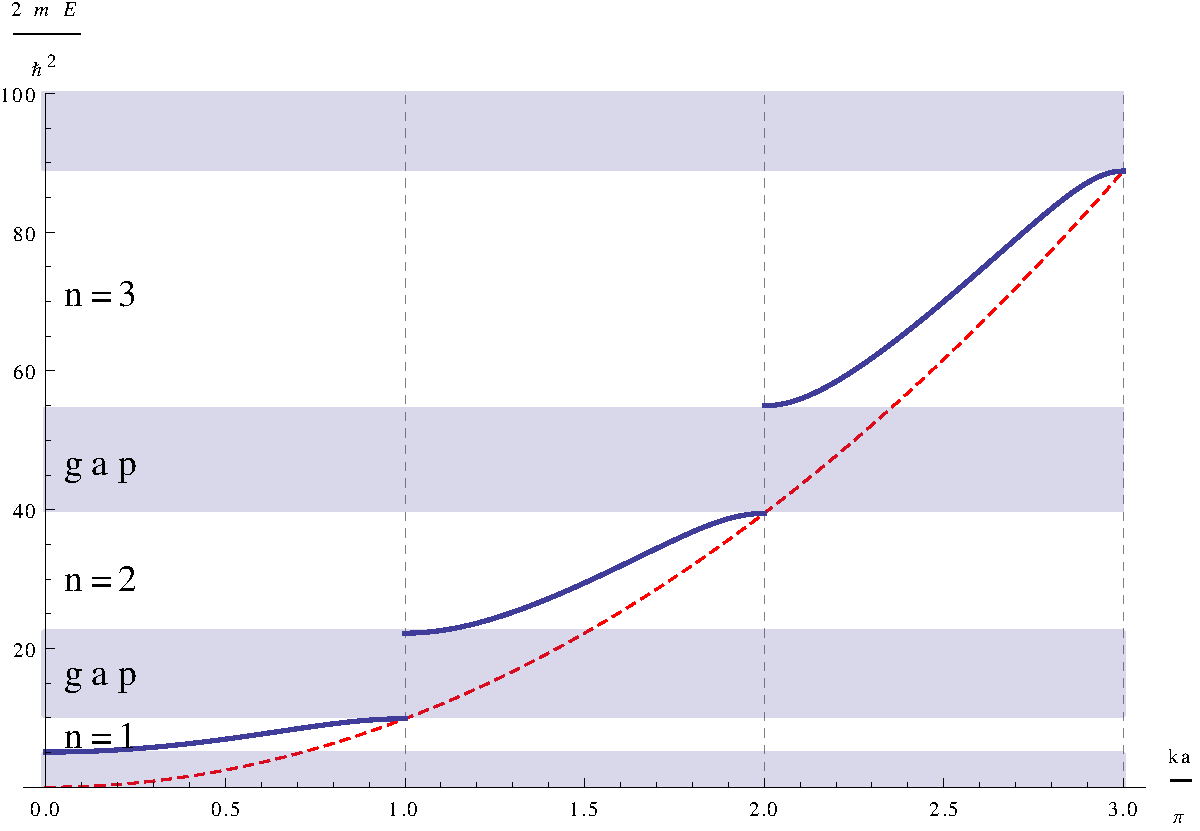
\includegraphics[width=0.45\hsize]{zones_ext.pdf}}
%  \caption{The energy bands plotted in a reduced (a) and extended (b) zone schemes. The energy gap at the edges of the BZ is shown in grey. The bands are numbered $1,2,3,...$.}
%  \label{fig:zones}
%\end{figure}

\marginfig[-3.2in]{zones_ext_red.png}{Extended and reduced zone schemes of the band structure. \label{fig:zones_ext_ref}}

The areas in grey are called the "gap" because there are no energy states there. So the density of states in the gap is zero. Outside the grey areas, for a given value of $k$, there are several solutions $E_{n}(k)$. The index $n$ specifies which solution is used. $n$ is the band index.\nl
For a given band $n$, there is a range of energies $E_{min}^n\le E \le E_{max}^n$ that solve the Schr{\"o}dinger equation. All energies in that range are in the $n$'th band. \nl
Remarkably, our solution of the Kronig-Penney model shows the behavior many real solid show: certain energies, lying in bands, are allowed. Between the bands there are energy gaps (sometimes called band-gaps). But what is the meaning of this spectrum ?

\section{Metal vs. Insulator}
We can now approach the question of how to differentiate between metal (ie. conductor) and insulator. Let us first recall Pauli's exclusion principle: each quantum state can be occupied by at most one electron. Forgetting spin for now (it only adds a $\times 2$ degeneracy), the quantum state of a Bloch electron is characterized by two numbers: $n$ the band index and $k$ the crystal momentum.\nl
Consider a solid at zero temperature. We now start filling it with unbound electrons. Starting from the lowest available energy, each electron takes a higher energy state corresponding to the $E_{n=1}(k)$ relation and the quantization of the $k$ states. When the $n=1$ band is filled, we continue to the $n=2$ band, etc. At some point the last electron has been placed. It could be in the $n=1$ band or it can be in a higher band. Regardless, this last electron's energy is the Fermi energy. Now we apply a weak electric field which accelerates the electrons, meaning that it gives them more energy. So we can ask: can the highest lying electron be accelerated? To answer this question we need to look at the Fermi energy. \nl
If the Fermi energy is in the middle of a band, then there are energy states available immediately above the Fermi energy and so electrons near the Fermi energy can be pushed easily to these energy states. This is a conductor.\nl
But if the Fermi energy is at the top of a band then there are no energy states to accelerate the top electrons to ! So when an electric field is applied, the electrons can not accelerate and there is no current. This is an insulator. \nl
Fig. \ref{fig:metal_vs_insulator} shows these two cases and another case where there is an overlap of bands resulting in a metallic behavior.\nl
The lower band, which is completely full is sometimes called the valence band, and the higher, partially empty band is called the conductance band. But that is not because all conductance happens at the conductance band! That is only the case at zero temperature. In the next chapter we will see how the conductance relates to the number of electrons in the conductance band and the number of holes left in the valence band. Together, they are the number of \emph{charge carriers}. We can think of the holes as particles with positive charge and in some materials the current is carried by the positive holes instead of the negative electrons.\nl
%\begin{figure}[!ht] 
%  \centering
%  \subfigure[]{\includegraphics[width=0.32\hsize]{insmetal1.pdf}}
%  \subfigure[]{\includegraphics[width=0.32\hsize]{insmetal2.pdf}}
%  \subfigure[]{\includegraphics[width=0.32\hsize]{insmetal3.pdf}}
%  \caption{The band structure of a metal vs. insulator. The shaded areas signify occupied electron states. (a) Insulator: the valence band is full with $E_F=2$ and the conduction band is empty. The Fermi Energy $E_F$ it at the top of the valence band. (b) Metal: because $E_F=2$ overlaps the second band. If the overlap is small with relatively few states involved, we speak of a semimetal. (c) Metal: because the higher electron means that now $E_F=4$ which extends to the next band, which isn't full.}
%  \label{fig:metal_vs_insulator}
%\end{figure}

\begin{figure}[!ht] 
  \centering
  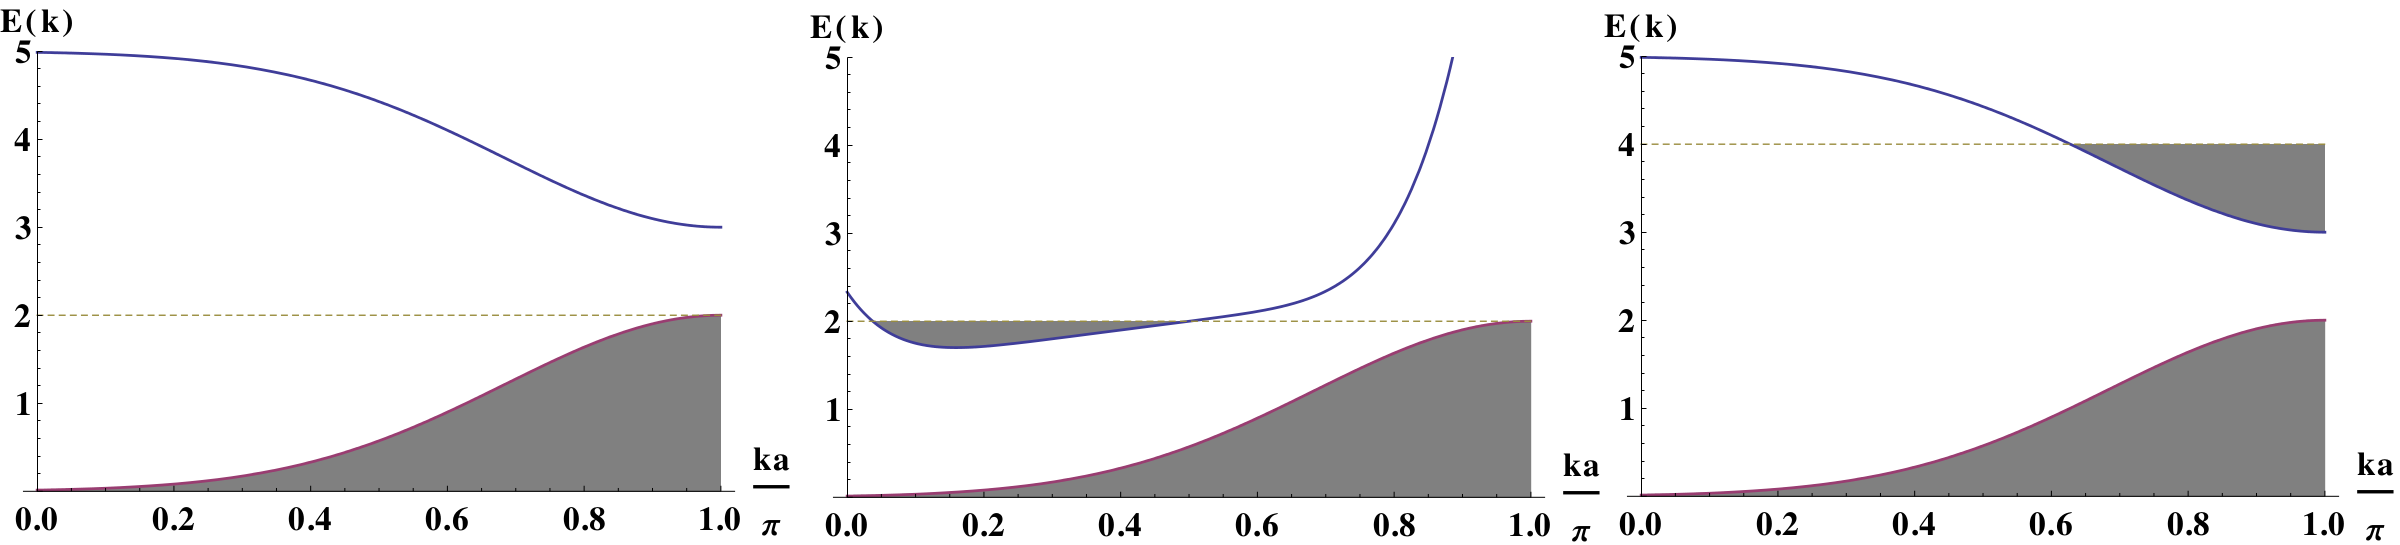
\includegraphics[width=15cm]{insmetal.png}
  \caption{The band structure of a metal vs. insulator. The shaded areas signify occupied electron states. (a) Insulator: the valence band is full with $E_F=2$ and the conduction band is empty. The Fermi Energy $E_F$ it at the top of the valence band. (b) Metal: because $E_F=2$ overlaps the second band. If the overlap is small with relatively few states involved, we speak of a semimetal. (c) Metal: because the higher electron means that now $E_F=4$ which extends to the next band, which isn't full.}
  \label{fig:metal_vs_insulator}
\end{figure}

\section{Measuring the gap, optical absorption}
As we discussed, at zero temperature insulators have no electrons in the conduction band and therefore no way for them to respond to weak electric field. Of course a strong enough field can tear electrons across the gap but it can have many other effects which will be hard to separate out. So to make the insulator conducting, we need a way to move electrons across the gap and into the conduction band. What will be left in their place are "holes". There are two main mechanisms by which electrons can be moved across the gap:
\begin{itemize}
\item Temperature can make the electrons jump across the gap. The probability for such a jump is approximately $e^{-\frac{E_g}{2k_BT}}$ with $E_g$ the gap energy.
\item A photon can be absorbed by an electron thereby increasing its energy.
\end{itemize} 
We will talk about temperature soon, we will ignore its effect for now. This leaves us with photon excitations.\nl
We can measure the gap $E_g$ as the frequency $\omega_g$ that electromagnetic radiation gets absorbed by the material. The photon energy is $\hbar\omega_g$: when radiating an insulator at this frequency (or a higher frequency), the photons will be absorbed; the valence electrons will jump to the conduction band; the conductivity of the material will rise. \nl
There are cases when the gap is indirect: the bottom of the conduction band is not at the same $k$ as the top of the valence band. In such a case photons aren't enough because their momentum is so small. Instead, a combination of absorption of both photon (for energy) and phonon (a lattice vibration, for momentum) are needed. See Fig. \ref{fig:optical_absorption} for a sketch of the two processes. 
\begin{figure}[!ht] 
  \centering
%  \subfigure[]{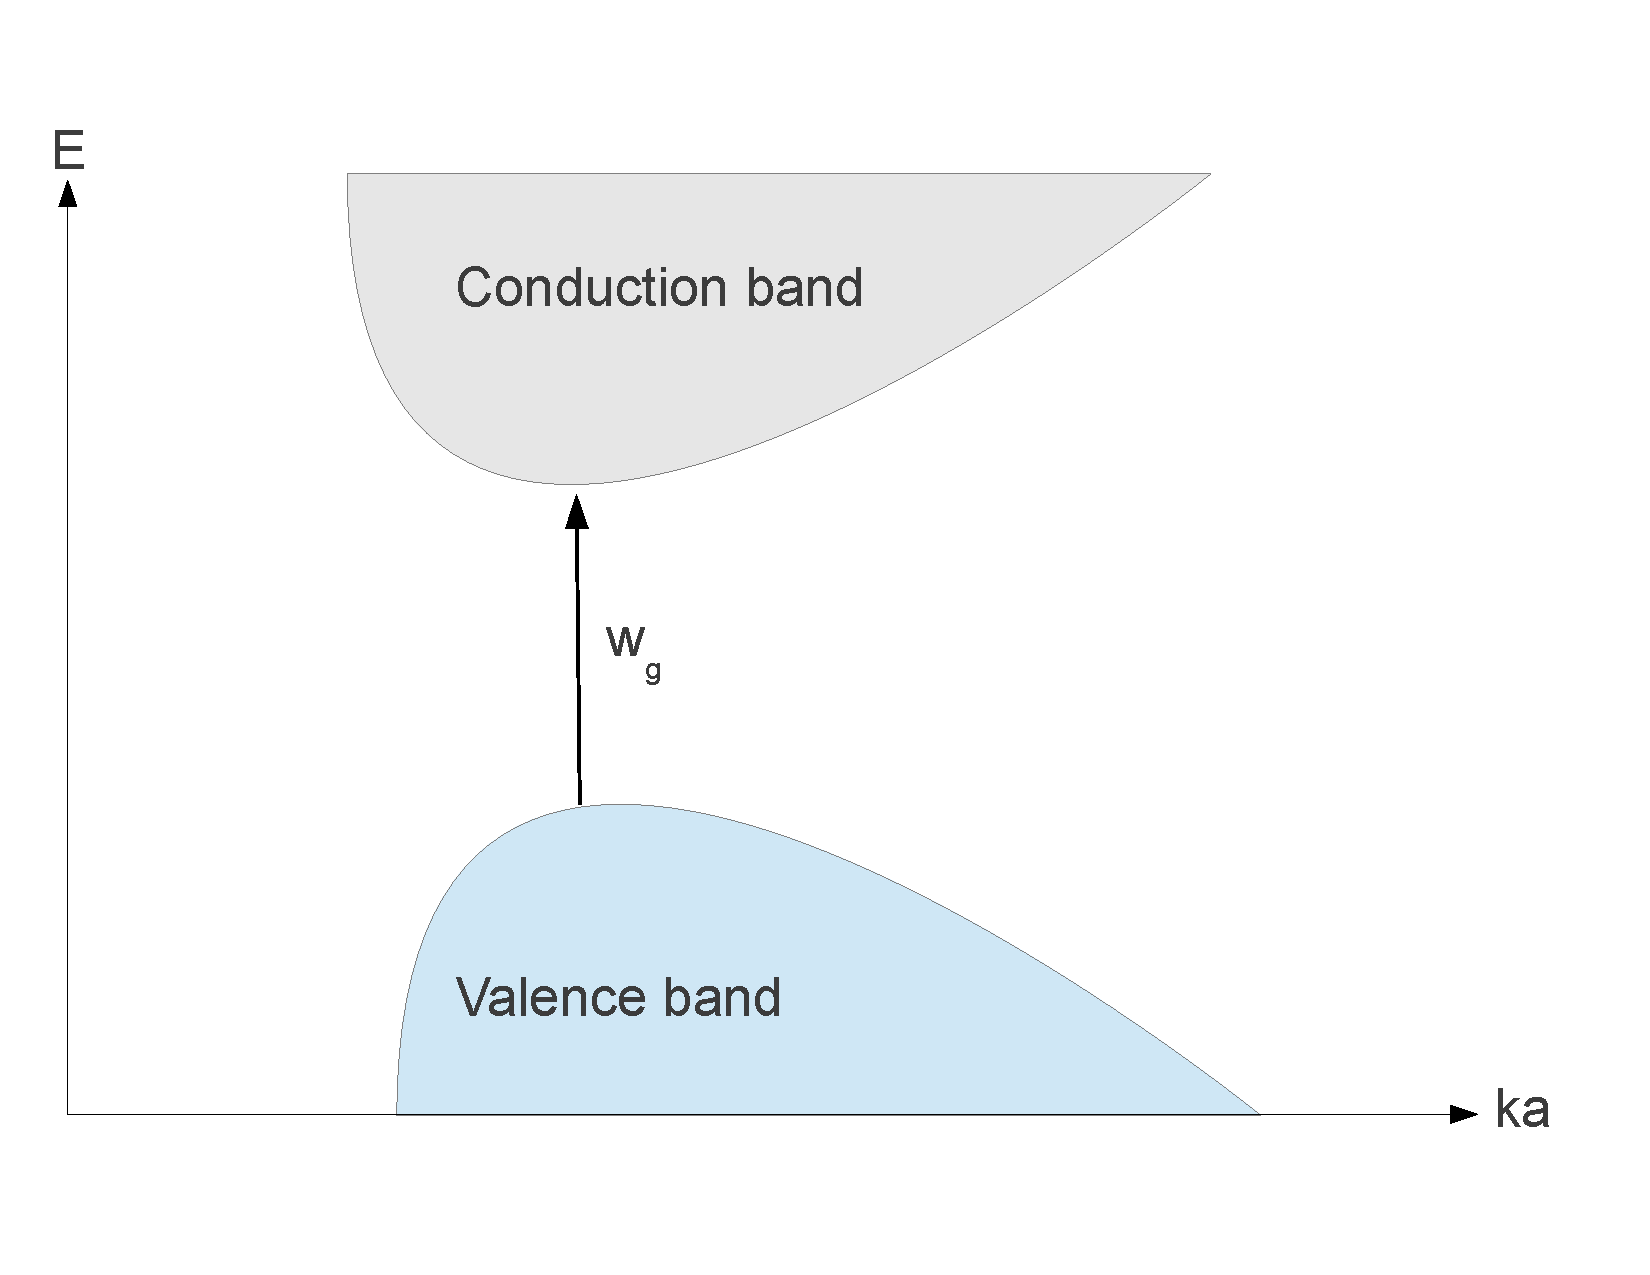
\includegraphics[width=0.49\hsize]{absorption1.pdf}}
%  \subfigure[]{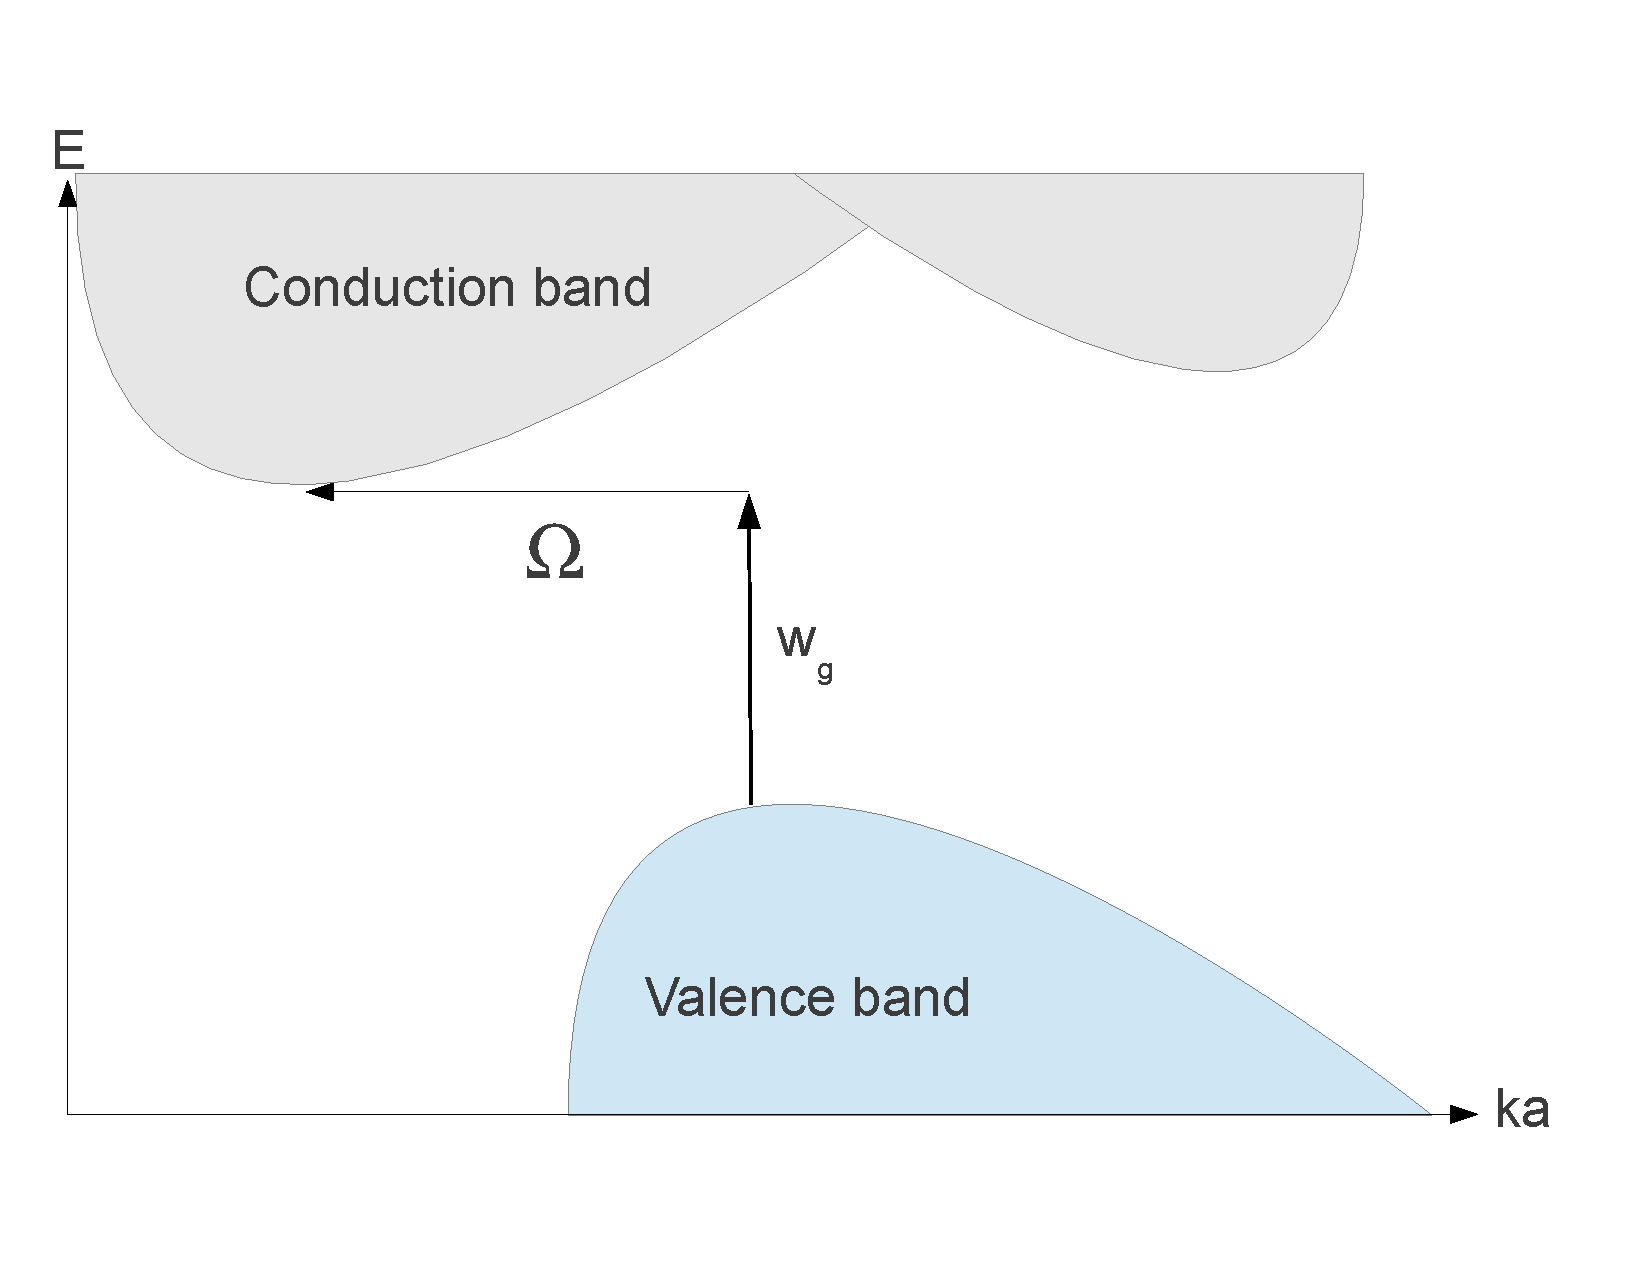
\includegraphics[width=0.49\hsize]{absorption2.pdf}}
  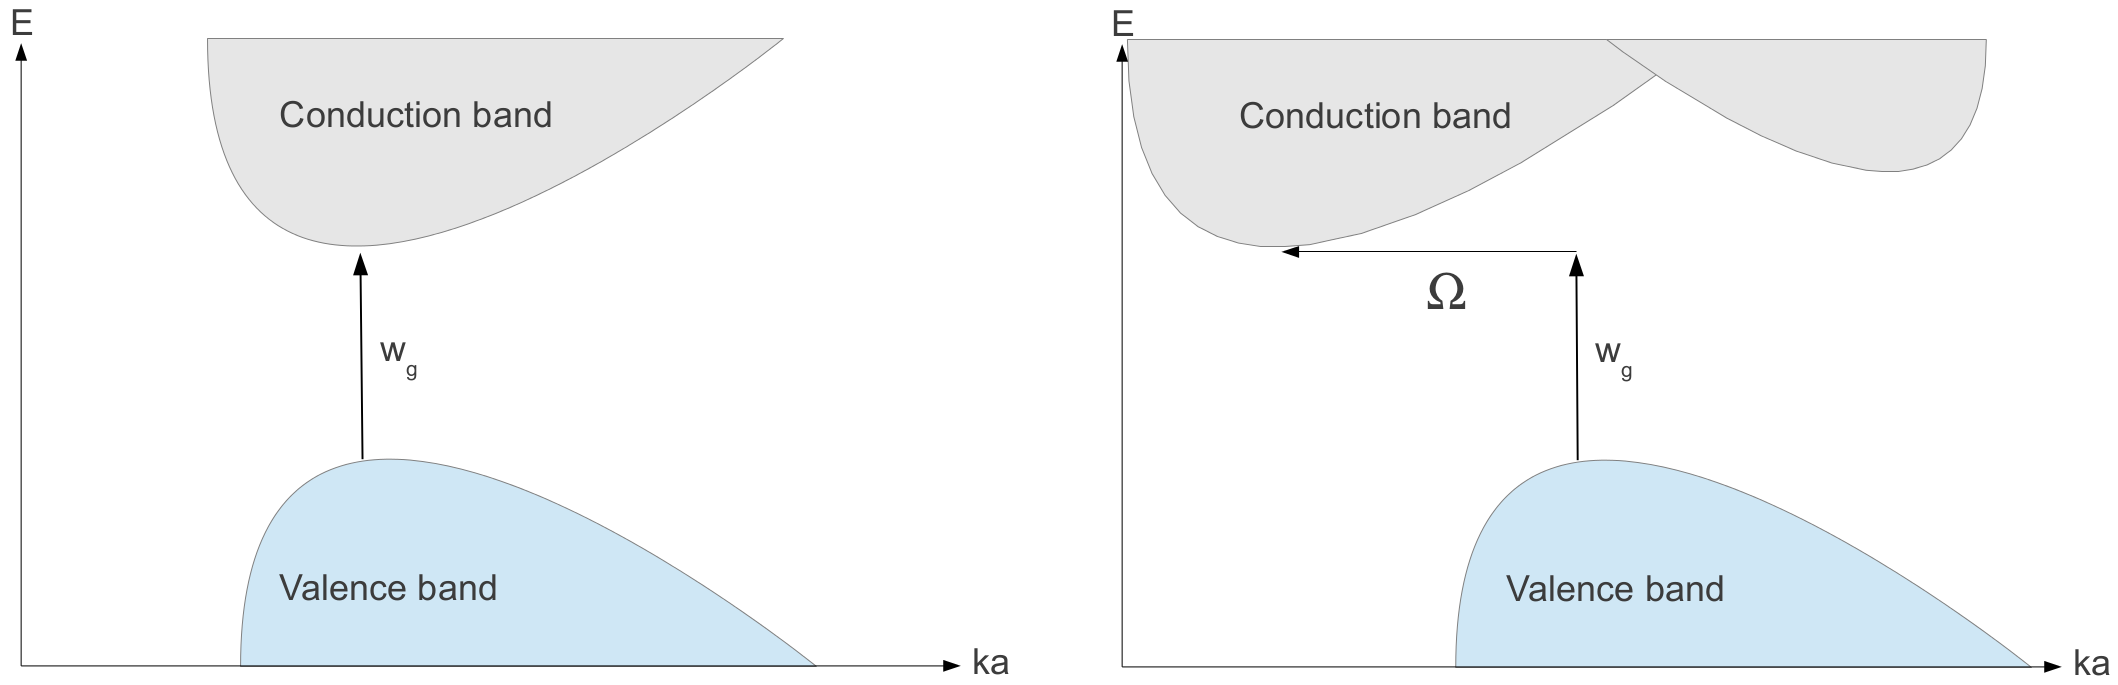
\includegraphics[width=15cm]{optical_absorptions}
  \caption{\textbf{Left:} The lowest point in the conduction band occurs at the same value of $k$ as the highest point in the valence band. A direct optical transition is possible and is drawn vertically with no significant change in $k$ because the photon has a small momentum. The threshold $\omega_g$ determines the energy gap $E_g = \hbar\omega_g$. \textbf{Right:} The indirect transition involves both a photon (for energy) and phonon (for momentum). The threshold energy is now $\hbar \omega_g = E_g - \hbar \Omega$ with $\Omega$ the frequency of the \emph{phonon} of wavevector $k_c$. }
  \label{fig:optical_absorption}
\end{figure}


\section{Insulator vs. Semiconductor}
So far we have made the following distinction between metal and insulator: at zero temperature, all bands of an insulator are either completely full or completely empty; a metal has at least one band which is partially filled.

When the temperature $T>0$, there is a probability for the electrons to be \emph{thermally excited} from the valence band to the conduction band, leaving behind them holes. Both the holes left behind and the electrons in the conduction band can then conduct electricity.

Whether the thermal effect leads to appreciable conductivity depends on the size of the gap. The probability to excite an electron across a gap $E_g$ is approximately $e^{-E_g/2k_bT}$. This means that for a gap energy of $4$eV at room temperature ($k_B T \approx 0.025$eV) this gives a probability of $e^{-80}\approx 10^{-35}$, a very small probability indeed. Compared with approximately $10^{22}$ electrons in the solid, this means that essentially no electrons get carried across the gap.

\noindent But if $E_g=0.25$eV, the probability at room temperature is $e^{-5}\approx 10^{-2}$ which will give observable conductance.

Solids that are insulators at $T=0$ but whose energy gap is small enough that thermal excitations (at reasonable temperatures) cause observable conductivity are called \emph{semiconductors}. The distinction between insulator and semiconductor is not a sharp one, but roughly speaking, the energy gap in most important semiconductors is less than $2$eV and often a few tenths of an eV. Typical room temperature resistivities of semiconductors are between $\rho \in [10^{-3},10^{9}]$ ohm-cm; metal have $\rho \approx 10^{-6}$ohm-cm; good insulators have $\rho\approx 10^{22}$ohm-cm.

Since the number of carriers varies exponentially with $1/T$, the conductivity of a semiconductor should \emph{increase} very rapidly as a function of temperature, in contrast to metals. Metals show a \emph{decrease} in conductivity with temperature because the electrons scatter of phonons.

\noindent Here are some typical values of the gap for (undoped) semiconductors at room temperature:

\noindent Silicon: 1.12eV

\noindent Germanium: 0.67eV

\noindent GaAs: 1.4eV

\noindent The study of the relation between carrier density and conductivity will be the subject of the next chapter.
%%%%%%%%%%%%%%%%%%%%%%%%%%%%%%%%%%%%%%%%%%%%%%%%%%%%%%%%%%%%%%%%%%%%%%%%%%%%%%%%%%%%%%%%%

\chapter{Conduction}
\personfeature[-2in]{Drude}{Paul Karl Ludwig Drude}{1863-1906}{was a German physicist specializing in optics. He wrote a fundamental textbook integrating optics with Maxwell's theories of electromagnetism. In 1894 he was responsible for introducing the symbol "c" for the speed of light in a perfect vacuum. In 1900 he developed a powerful model to explain the thermal, electrical, and optical properties of matter. The Drude model would be further advanced in 1933 by Arnold Sommerfeld and Hans Bethe. In 1906, at the height of his career, he became a member of the Prussian Academy of Sciences. A few days after his inauguration lecture, for inexplicable reasons, he committed suicide. \href{http://en.wikipedia.org/wiki/Paul_Karl_Ludwig_Drude}{(Wikipedia)}}

\lettrine[lines=3,slope=6pt,nindent=6pt]{\initfamily T}{h}e metallic state has proven to be one of the great fundamental states of matter: over 2/3 of the elements are metals. Starting from the 19th century, physicists have been trying to construct simple models to explain the metallic state. During this time, many unknowns had to wait for quantum mechanics to be discovered. Yet some classical theories survived, and when properly used, are very instructive, even when the assumptions behind them are known to be wrong. The Drude model is exactly such a case: it is still used today to understand conductance on a general and simple way; Even though it is known to be wrong, it can still capture some essential physics.
\section{Drude - classically explaining conduction.}
In 1897, Thompson discovered the electron. Three years later Drude constructed his theory of electrical and thermal conduction. Drude's assumptions were:
\begin{itemize}
\item When atoms of a metallic element are brought together, some of the electrons become detached and wander freely through the metal, whereas the ions (the nucleus plus core electrons) remain static. 
\item Between collisions, the interaction of a given electron with both the other electrons and the ions, are neglected. Therefore, in the absence of an external electromagnetic field, the electron moves in a straight line between collisions. When such a field is present, the electron obeys Newton's laws in accordance with the Lorentz law of electric force. So Drude's is a free electron theory.
\item Collisions are instantaneous events that abruptly alter the velocity of the electron. Drude attributed them to electrons bouncing off the impenetrable ion cores. We've already learned about electrons in a periodic potential so we understand just how wrong this picture is. In quantum theory the electron waves know about the periodic potential of the lattice and obey Bloch's theorem: there is no scattering with the ions at all. Instead, quantum mechanically, important contributions come from scattering of electrons from lattice impurities and from lattice vibrations (phonons). Fortunately, in many cases it doesn't matter what the electrons scatter against, as long as there is some scattering mechanism.
\item The electron experiences a collision with a probability $1/\tau$ per unit time. This means that for the interval $dt$, the probability for one collision is $dt/\tau$. (Poisson process). It also means that an electron travels on average time $\tau$ between collisions. 
\item After a collision the electron sets off in a completely random direction with a velocity which is related to the temperature at the location of the collision.
\end{itemize}  
We define the resisitivity $\rho$ as the proportionality factor between the electric field and the current density it induces:
\be 
\vec{E} = \rho \vec{j}
\ee
Similarly, we can define the conductivity $\sigma$ as the inverse of $\rho$ so that,
\be 
\vec{j} = \sigma \vec{E} \outnote{Ohm's Law}
\ee
The result above is Ohm's law.\nl
The current density is 
\be
\vec{j} = -ne\vec{v} 
\label{eq:current}
\ee
because this is the number of electrons passing through a surface per area per time. \nl
The net current density is given by Eq. \ref{eq:current}. In the absence of an electric field, electrons have equal probability to move in all directions, so the net velocity is zero and therefore the net current is zero. But in the presence of an electric field $\vec{E}$, there will be a mean electronic velocity directed opposite to the field (because the electron charge is negative).\nl
The Coulomb force the electrons experience accelerates them as,
\be
\dot{\vec{v}} = -\frac{e\vec{E}}{m}
\ee
So that the velocity of an electron after accelerating for time $\tau$ is,
\be 
\vec{v} = \vec{v}_0 - \frac{e\vec{E}\tau}{m}
\ee
But the velocity at time 0 (immediately after collision) is zero, $\vec{v}_0=0$, because on average after a collision it moves in any direction. So, we have,
\bea
\vec{j} &=& \frac{ne^2\tau}{m} \vec{E} = \sigma \vec{E}\nn
\sigma &=& \frac{ne^2\tau}{m} \outnote{Drude conductivity}
\eea
The formula above defines the Drude conductivity. We see that it is proportional to both the number of carriers $n$, and the microscopic relaxation time, $\tau$. The fact that the conductivity depends on two unknowns is inconvenient when comparing theory to experiment. What can be done about it?
\section{The Hall Effect}
\personfeature[-0.7in]{Edwin_Hall}{Edwin Herbert Hall}{1855-1938}{was an American physicist who discovered the "Hall effect". Hall conducted thermoelectric research at Harvard and also wrote numerous physics textbooks and laboratory manuals. The Hall effect was discovered by Hall in 1879, while working on his doctoral thesis in Physics. \href{http://en.wikipedia.org/wiki/Edwin_Hall}{(Wikipedia)}}
In the last section we learned about the Drude model and how it tries to explain conductance. But the whole idea of electrons scattering off the ions is quantum-mechanically wrong. Instead, they scatter off lattice impurities and lattice vibrations (phonons). This means that carefully prepared samples (extremely clean) tested at very low temperatures can allow the electrons to travel several centimetres between collisions: ie. they can pass an order of $10^8$ interatomic spacings between collisions! Since $\tau$ is so difficult to estimate theoretically, it is better if we can find observables that do not depend on $\tau$. The (classical) Hall effect gives us what we need.

Before we start, it is important to stress that the classical theory of electrons in a magnetic field suffers from many drawbacks. A correct quantum-mechanical treatment of magnetic field is crucial to understand many important effects, but is outside the scope of this course. The quantum Hall effect is a subject on ongoing research to this day with many puzzles remaining. It is a serious candidate for implementing quantum computing, though there are still (possibly huge) obstacles that need to be surmounted.

\noindent In 1879, E.W. Hall tried to see what happens to current when it is subjected to a magnetic field. Fig. \ref{fig:Hall} shows the setup of Hall's experiment.\nl
\begin{figure}[!ht] 
  \centering
  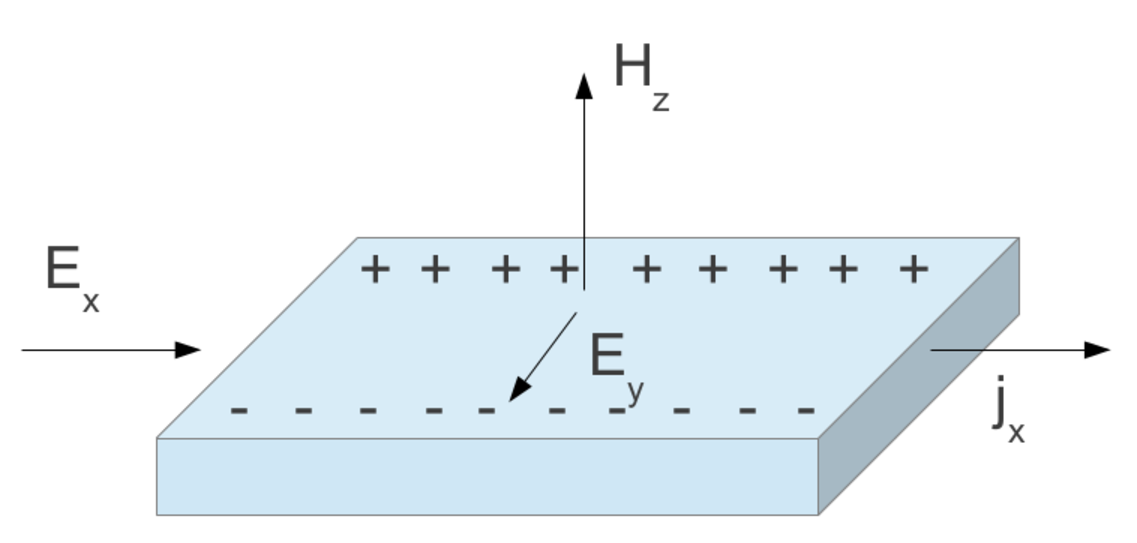
\includegraphics[width=12cm]{Hall2.pdf}
  \caption{Schematic view of Hall's experiment.}
  \label{fig:Hall}
\end{figure}
There are two quantities of interest: 
\be
\rho(H) = \frac{E_x}{j_x}
\ee
is the (transverse) magneto-resistance. It is an important quantity but we will not discuss it here.\nl
The second is the size of the electric field $E_y$ created because of the electron drift. It is related to both the current $j_x$ and the magnetic field $H$, so we define the Hall coefficient:
\be 
R_H = \frac{E_y}{j_x H} \outnote{Hall coefficient}
\ee
Note that since the Hall field is in the negative $y$ direction, $R_H$ should be negative. But if the charge carriers were positive, the sign of $j_x$ would be reversed so the Hall coefficient becomes positive. This is very important because it means the sign of the Hall coefficient can be used to determine the sign of the charge carriers. When conductance is done by holes instead of electrons, $R_H>0$.\nl
Let us calculate the Hall coefficient by solving the equations of motion for the electrons. For a short enough $dt$, the probability an electron will have a collision is $\frac{dt}{\tau}$, so the probability it doesn't have a collision is $1-\frac{dt}{\tau}$. Applying an external force $\vec{F}$, in the collision (Drude) model, we have,
\bea 
\vec{p}(t+dt) &=& \left(1-\frac{dt}{\tau} \right)\left(\vec{p}(t) + \vec{F}dt + O(dt^2) \right) + \frac{dt}{\tau}\vec{F}\,O(dt) \nn
\vec{p}(t+dt) &=& \vec{p}(t) - \frac{dt}{\tau}\vec{p}(t) + \vec{F}dt + O(dt^2)
\eea
The first term in the top equation is the contribution of an electron that didn't collide at time $dt$, the second term is if it did. Taking $dt$ small enough that we keep only terms linear in $dt$, we have,
\be 
\dot{\vec{p}}(t) = -\frac{\vec{p}(t)}{\tau} + \vec{F}
\ee
The collision term $\tau$ appears as a correction to Newton's usual $\dot{p} = F$. It is sometimes called the "relaxation time approximation". You may know it as a "friction" term with the friction coefficient $\sim \frac{1}{\tau}$.\nl
%Notice that for normal acceleration of the electron in an electric field this gives,
%\bea
%\dot{\vec{v}}(t) &=& -\frac{1}{\tau}\vec{v}(t) -\frac{e\vec{E}}{m} \nn
%\vec{v}(t) &=& \vec{b} e^{-t/\tau} \nn
%\dot{\vec{v}}(t) &=& \dot{\vec{b}} e^{-t/\tau} -\frac{1}{\tau} \vec{v} = -\frac{1}{\tau}\vec{v} -\frac{e\vec{E}}{m} \nn
%\dot{\vec{b}}  &=& -\frac{eE}{m} e^{t/\tau}\nn
%\vec{b} &=& -\frac{eE\tau}{m} \left( e^{t/\tau} + C \right) \nn
%\vec{v} &=& -\frac{eE\tau}{m}\left(1+e^{-t/\tau}C\right) \nn
%\vec{v}(t\rightarrow -\infty) &=& 0 \quad \rightarrow \quad C = 0 \nn
%\vec{v}(t) &=& -\frac{eE\tau}{m}
%\eea
%This is exactly the result we hand-waved before.\nn
Now, placing the electrons in electric and magnetic fields gives the Lorentz force,
\be 
\vec{F} = -e\left(\vec{E} - \frac{\vec{p}\times\vec{H}}{mc} \right)
\ee
so that we're trying to solve,
\be 
\dot{\vec{p}}(t) = -\frac{\vec{p}(t)}{\tau} -e\left(\vec{E} - \frac{\vec{p}\times\vec{H}}{mc} \right)
\ee
At steady state, the solution doesn't change with time so $\dot{\vec{p}}=0$. This gives,
\bea
0 &=& -e E_x -\omega_c p_y -\frac{p_x}{\tau}\nn
0 &=& -e E_y +\omega_c p_x -\frac{p_y}{\tau}\nn
\omega_c &=& \frac{eH}{mc} \outnote{Cyclotron frequency}
\eea
Multiplying both equations by $-\frac{ne\tau}{m}$ we have,
\bea
\sigma E_x &=& \omega_c \tau j_y + j_x \nn
\sigma E_y &=& -\omega_c \tau j_x + j_y \nn
\eea
But there is no current in the $y$ direction, so $j_y=0$ and 
\bea 
E_y &=& -\left(\frac{\omega_c \tau}{\sigma}\right)j_x = -\left(\frac{H}{nec}\right)j_x \nn
R_H &=& \frac{E_y}{j_x H} = -\frac{1}{nec} \outnote{Hall coefficient}
\eea
We have reached an important conclusion! That the Hall coefficient depends only on the density of charge carriers and its sign depends on whether they are negative or positive. By measuring the Hall coefficient one can determine these values experimentally, without needing to know the time $\tau$ between collision, or the collision mechanism.\nl
Note: We have assumed that the electron density $n$ doesn't depend on $H$. In general, it does, so this is again an oversimplification, but it gives some of the correct qualitative physics.

%%%%%%%%%%%%%%%%%%%%%%%%%%%%%%%%%%%%%%%%%%%%%%%%%%%%%%%%%%%%%%%%%%%%%%%%%%%%%%%%%%%%%%%%%
\chapter{Summary}
\lettrine[lines=3,slope=6pt,nindent=6pt]{\initfamily W}{e}'ve had a challenging one-semester journey through some aspects of modern physics. In our journey, we have learned about the following:
\begin{itemize}
\item Some of the physical motivations to develop a quantum theory to replace the classical physics. The so-called wave/particle duality.
\item The Schr{\"o}dinger equation and how to use it to solve simple quantum mechanical models.
\item Potential wells: quantization of momentum and energy. The Fermi energy. Density of states and how to use it for calculations.
\item Scattering, tunnelling. The importance of tunnelling as a source of problems and as a means for accurate measurements.
\item The foundations of quantum mechanics: the uncertainty principle and non-commuting variables, the postulates, physical observables as operators, Dirac notation.
\item The quantum harmonic oscillator: how to solve it and a taste on how it relates to physical systems: its connection to lattice vibrations (phonons) and quanta of electromagnetic energy (photons).
\item Solids and their crystal form.
\item Band theory of solids: the difference between metal, insulator and semiconductor.
\item Classical description of conductance and the use of the Hall effect to measure the sign and density of charge carriers.
\end{itemize}


\noindent It is a long list of basic topics. We have not compromised on the physical content but we have limited ourselves to the simplest possible examples. Don't let the simplicity of the calculations fool you! We have touched some tricky and deep mysteries that took the best minds of the $20^{th}$ century to solve. The course material covers the essential starting point for the quantum theory of solids. It is up to you to take the challenge !

\noindent Some of the topics we didn't discuss:
\begin{itemize}
\item The effect of temperature: thermodynamics / statistical mechanics. What is a current? What is heat?
\item The hydrogen atom - the Schr{\"o}dinger equation in a spherical potential.
\item Electron spin and magnetic field.
\item Laser physics.
\item Better understanding of the band theory of solids and the effect of a weak periodic potential on electron wave-
functions.
\item The failures of the classical theory of conduction. Correct quantum description of conductance. Semiclassical description, effective mass.
\item Electron-electron interactions and how they lead to magnetism and superconductivity.
\end{itemize}
All of the above topics are interesting and have important uses in today's technology. Some of them need only a little more work, others take years to learn properly. I hope that what we did learn made you interested enough to want to learn more.

\textsl{"Science is facts; just as houses are made of stones, so is science made of facts; but a pile of stones is not a house and a collection of facts is not necessarily science."}\\
 - \textbf{Henri Poincare}



%%%%%%%%%%%%%%%%%%%%%%%%%%%%%%%%%%%%%%%%%%%%%%%%%%%%%%%%%%%%%%%%%%%%%%%%%%%%%%%%%%%%%%%%%



%
%\bibliography{RRNbib}
%\bibliographystyle{unsrt}

\end{document}

% %%%%%%%%%%%%%%%%%%%%%%%%%%%%%%%%%%%%%%%%%%%%%%%%%%%%%%%%%%%%%%%

